%% abtex2-modelo-trabalho-academico.tex, v-1.9.7 laurocesar
%% Copyright 2012-2018 by abnTeX2 group at http://www.abntex.net.br/ 
%%
%% This work may be distributed and/or modified under the
%% conditions of the LaTeX Project Public License, either version 1.3
%% of this license or (at your option) any later version.
%% The latest version of this license is in
%%   http://www.latex-project.org/lppl.txt
%% and version 1.3 or later is part of all distributions of LaTeX
%% version 2005/12/01 or later.
%%
%% This work has the LPPL maintenance status `maintained'.
%% 
%% The Current Maintainer of this work is the abnTeX2 team, led
%% by Lauro César Araujo. Further information are available on 
%% http://www.abntex.net.br/
%%
%% This work consists of the files abntex2-modelo-trabalho-academico.tex,
%% abntex2-modelo-include-comandos and abntex2-modelo-references.bib
%%

% ------------------------------------------------------------------------
% ------------------------------------------------------------------------
% abnTeX2: Modelo de Trabalho Academico (tese de doutorado, dissertacao de
% mestrado e trabalhos monograficos em geral) em conformidade com 
% ABNT NBR 14724:2011: Informacao e documentacao - Trabalhos academicos -
% Apresentacao
% ------------------------------------------------------------------------
% ------------------------------------------------------------------------

\documentclass[
	% -- opções da classe memoir --
	12pt,				% tamanho da fonte
	openright,			% capítulos começam em pág ímpar (insere página vazia caso preciso)
	oneside,			% para impressão em recto e verso use 'twoside'. Oposto a 'oneside'
	a4paper,			% tamanho do papel. 
	% -- opções da classe abntex2 --
	%chapter=TITLE,		% títulos de capítulos convertidos em letras maiúsculas
	%section=TITLE,		% títulos de seções convertidos em letras maiúsculas
	%subsection=TITLE,	% títulos de subseções convertidos em letras maiúsculas
	%subsubsection=TITLE,% títulos de subsubseções convertidos em letras maiúsculas
	% -- opções do pacote babel --
	english,			% idioma adicional para hifenização
	brazil				% o último idioma é o principal do documento
	]{abntex2}

% ---
% Pacotes básicos 
% ---
\usepackage{lmodern}			% Usa a fonte Latin Modern			
\usepackage[T1]{fontenc}		% Selecao de codigos de fonte.
\usepackage[utf8]{inputenc}		% Codificacao do documento (conversão automática dos acentos)
\usepackage{indentfirst}		% Indenta o primeiro parágrafo de cada seção.
\usepackage{color}				% Controle das cores
\usepackage{graphicx}			% Inclusão de gráficos
\usepackage{microtype} 			% para melhorias de justificação
\usepackage{minted}          % inclusão de codigo
% ---
		
% ---
% Pacotes adicionais, usados apenas no âmbito do Modelo Canônico do abnteX2
% ---
\usepackage{lipsum}				% para geração de dummy text
% ---

% ---
% Pacotes de citações
% ---
\usepackage[brazilian,hyperpageref]{backref}	 % Paginas com as citações na bibl
\usepackage[alf, abnt-etal-list=0]{abntex2cite}	% Citações padrão ABNT
\citebrackets()

% --- 
% CONFIGURAÇÕES DE PACOTES
% --- 

% ---
% Configurações do pacote backref
% Usado sem a opção hyperpageref de backref
\renewcommand{\backrefpagesname}{Citado na(s) página(s):~}
% Texto padrão antes do número das páginas
\renewcommand{\backref}{}
% Define os textos da citação
\renewcommand*{\backrefalt}[4]{
	\ifcase #1 %
		Nenhuma citação no texto.%
	\or
		Citado na página #2.%
	\else
		Citado #1 vezes nas páginas #2.%
	\fi}%
% ---

% ---
% Informações de dados para CAPA e FOLHA DE ROSTO
% ---
\titulo{Prótotipo de Criação Flexível de Dashboards Interativos e Coordenados}
\autor{Elvis Thermo Carvalho Miranda}
\local{Belém}
\data{2021}
\orientador{Carlos Gustavo Resque dos Santos}
\coorientador{Bianchi Serique Meiguins}
\instituicao{Universidade Federal do Pará}
\instituicaounidade{Instituto de Ciências Exatas e Naturais}
\instituicaosubunidade{Faculdade De Computação}


\tipotrabalho{Trabalho de Conclusão de Curso)}
% O preambulo deve conter o tipo do trabalho, o objetivo, 
% o nome da instituição e a área de concentração 
\preambulo{Trabalho de conclusão de curso de graduação apresentado ao Instituto de Ciências Exatas e Naturais da Universidade Federal do Pará como parte dos requisitos necessários para a obtenção do título de Bacharel em Sistemas de Informação}
% ---


% ---
% Configurações de aparência do PDF final

% alterando o aspecto da cor azul
\definecolor{blue}{RGB}{41,5,195}

% informações do PDF
\makeatletter
\hypersetup{
     	%pagebackref=true,
		pdftitle={\@title}, 
		pdfauthor={\@author},
    	pdfsubject={\imprimirpreambulo},
	    pdfcreator={LaTeX with abnTeX2},
		pdfkeywords={abnt}{latex}{abntex}{abntex2}{trabalho acadêmico}, 
		colorlinks=true,       		% false: boxed links; true: colored links
    	linkcolor=black,          	% color of internal links
    	citecolor=black,        		% color of links to bibliography
    	filecolor=black,      		% color of file links
		urlcolor=black,
		bookmarksdepth=4
}
\makeatother
% --- 

% ---
% Posiciona figuras e tabelas no topo da página quando adicionadas sozinhas
% em um página em branco. Ver https://github.com/abntex/abntex2/issues/170
\makeatletter
\setlength{\@fptop}{5pt} % Set distance from top of page to first float
\makeatother
% ---

% ---
% Possibilita criação de Quadros e Lista de quadros.
% Ver https://github.com/abntex/abntex2/issues/176
%
\newcommand{\quadroname}{Quadro}
\newcommand{\listofquadrosname}{Lista de quadros}

% \newfloat[chapter]{quadro}{loq}{\quadroname}
\newlistof{listofquadros}{loq}{\listofquadrosname}
\newlistentry{quadro}{loq}{0}

% configurações para atender às regras da ABNT
\setfloatadjustment{quadro}{\centering}
\counterwithout{quadro}{chapter}
\renewcommand{\cftquadroname}{\quadroname\space} 
\renewcommand*{\cftquadroaftersnum}{.\hfill}

\setfloatlocations{quadro}{hbtp} % Ver https://github.com/abntex/abntex2/issues/176
% ---

% --- 
% Espaçamentos entre linhas e parágrafos 
% --- 

% O tamanho do parágrafo é dado por:
\setlength{\parindent}{1.3cm}

% Controle do espaçamento entre um parágrafo e outro:
\setlength{\parskip}{0.2cm}  % tente também \onelineskip

% ---
% compila o indice
% ---
\makeindex
% ---

% ----
% Início do documento
% ----
\begin{document}

% Seleciona o idioma do documento (conforme pacotes do babel)
%\selectlanguage{english}
\selectlanguage{brazil}

% Retira espaço extra obsoleto entre as frases.
\frenchspacing 

% ----------------------------------------------------------
% ELEMENTOS PRÉ-TEXTUAIS
% ----------------------------------------------------------
% \pretextual

% ---
% Capa
% ---
\imprimircapa
% ---

% ---
% Folha de rosto
% (o * indica que haverá a ficha bibliográfica)
% ---
\imprimirfolhaderosto*
% ---

% ---
% Inserir a ficha bibliografica
% ---

% Isto é um exemplo de Ficha Catalográfica, ou ``Dados internacionais de
% catalogação-na-publicação''. Você pode utilizar este modelo como referência. 
% Porém, provavelmente a biblioteca da sua universidade lhe fornecerá um PDF
% com a ficha catalográfica definitiva após a defesa do trabalho. Quando estiver
% com o documento, salve-o como PDF no diretório do seu projeto e substitua todo
% o conteúdo de implementação deste arquivo pelo comando abaixo:
%
% \begin{fichacatalografica}
%     \includepdf{fig_ficha_catalografica.pdf}
% \end{fichacatalografica}

\begin{fichacatalografica}
	\sffamily
	\vspace*{\fill}					% Posição vertical
	\begin{center}					% Minipage Centralizado
	\fbox{\begin{minipage}[c][8cm]{13.5cm}		% Largura
	\small
	Solicite sua ficha catalográfica em: \url{http://bcficat.ufpa.br/}
	\end{minipage}}
	\end{center}
\end{fichacatalografica}
% ---

% ---
% Inserir errata
% ---
%\begin{errata}
%Elemento opcional da %\cite{NBR14724:2011}. Exemplo:

%\vspace{\onelineskip}

%FERRIGNO, C. R. A. \textbf{Tratamento de neoplasias ósseas apendiculares com
%reimplantação de enxerto ósseo autólogo autoclavado associado ao plasma
%rico em plaquetas}: estudo crítico na cirurgia de preservação de membro em
%cães. 2011. 128 f. Tese (Livre-Docência) - Faculdade de Medicina Veterinária e
%Zootecnia, Universidade de São Paulo, São Paulo, 2011.

%\begin{table}[htb]
%\center
%\footnotesize
%\begin{tabular}{|p{1.4cm}|p{1cm}|p{3cm}|p{3cm}|}
%  \hline
%   \textbf{Folha} & \textbf{Linha}  & \textbf{Onde se lê}  & \textbf{Leia-se}  \\
%    \hline
%    1 & 10 & auto-conclavo & autoconclavo\\
%   \hline
%\end{tabular}
%\end{table}

%\end{errata}
% ---

% ---
% Inserir folha de aprovação
% ---

% Isto é um exemplo de Folha de aprovação, elemento obrigatório da NBR
% 14724/2011 (seção 4.2.1.3). Você pode utilizar este modelo até a aprovação
% do trabalho. Após isso, substitua todo o conteúdo deste arquivo por uma
% imagem da página assinada pela banca com o comando abaixo:
%
% \begin{folhadeaprovacao}
% \includepdf{folhadeaprovacao_final.pdf}
% \end{folhadeaprovacao}
%
\begin{folhadeaprovacao}

  \begin{center}
    {\ABNTEXchapterfont\large\imprimirautor}

    \vspace*{\fill}\vspace*{\fill}
    \begin{center}
      \ABNTEXchapterfont\bfseries\Large\imprimirtitulo
    \end{center}
    \vspace*{\fill}
    
    \hspace{.45\textwidth}
    \begin{minipage}{.5\textwidth}
        \imprimirpreambulo
    \end{minipage}%
    \vspace*{\fill}
   \end{center}
        
   Conceito: \rule{3cm}{.1pt}
   
   \imprimirlocal, 1 de janeiro de 2019.
   
   \vspace{1cm}
   \begin{center}
   BANCA EXAMINADORA
   \end{center}
    

   \assinatura{\textbf{\imprimirorientador} - Orientador \\ UFPA}
   %\assinatura{\textbf{\imprimircoorientador} - Coorientador \\ UFPA}
   \assinatura{\textbf{Nome Convidado 1} \\ SIGLA INSTITUIÇÃO}
   \assinatura{\textbf{Nome Convidado 2} \\ SIGLA INSTITUIÇÃO}
   %\assinatura{\textbf{Nome Convidado 3} \\ SIGLA INSTITUIÇÃO}
      

  
\end{folhadeaprovacao}
% ---

% ---
% Dedicatória
% ---
\begin{dedicatoria}
   \vspace*{\fill}
   \centering
   \noindent
   \textit{ Escreva sua dedicatória aqui.} \vspace*{\fill}
\end{dedicatoria}
% ---

% ---
% Agradecimentos
% ---
\begin{agradecimentos}
Os agradecimentos principais são direcionados à Gerald Weber, Miguel Frasson,
Leslie H. Watter, Bruno Parente Lima, Flávio de Vasconcellos Corrêa, Otavio Real
Salvador, Renato Machnievscz e todos aqueles que
contribuíram para que a produção de trabalhos acadêmicos conforme
as normas ABNT com \LaTeX\ fosse possível.

Agradecimentos especiais são direcionados ao Centro de Pesquisa em Arquitetura
da Informação da Universidade de
Brasília (CPAI), ao grupo de usuários
\emph{latex-br} e aos
novos voluntários do grupo
\emph{\abnTeX} que contribuíram e que ainda
contribuirão para a evolução do \abnTeX.

\end{agradecimentos}
% ---

% ---
% Epígrafe
% ---
\begin{epigrafe}
    \vspace*{\fill}
	\begin{flushright}
		\textit{``Você pode até perder a fé nos outros, mas nunca em si mesmo.''\\
		(Optimus Prime)}
	\end{flushright}
\end{epigrafe}
% ---

% ---
% RESUMOS
% ---

% resumo em português
\setlength{\absparsep}{18pt} % ajusta o espaçamento dos parágrafos do resumo
\begin{resumo}
A visualização da informação pode ampliar a compreensão dos dados pelo usuário usando representações visuais, e os \textit{dashboards} são uma técnica conhecida para dividir dados em várias interfaces de comunicação, facilitando a tomada de decisão. Embora haja uma variedade de ferramentas e layouts, alguns aspectos do uso do painel são limitados ao domínio da codificação quando um usuário precisa de mais especificidade, como visualizações coordenadas e uso de visualizações de dados multivariadas. Este trabalho apresenta uma abordagem personalizável e coordenada usando dados multivariados em \textit{dashboards}. A partir de uma revisão da literatura observaram-se técnicas de visualização comumente usadas em ferramentas de criação de painéis, e essas técnicas são expandidas para dados multivariados em um ambiente coordenado e personalizável. O protótipo torna possível definir, o espaço para criar as visualizações conforme as necessidades e os pré-requisitos exigidos pelo usuário. Caracterizando as cores da maneira mais representativa para o banco de dados e fornece várias interações coordenadas como filtro, detalhes na demanda, destaque, seleção e configurações de colunas visíveis do banco de dados. Essa coordenação é feita no nível de interação, com seleções e filtros. Um protótipo usando essa abordagem foi construído e está disponível online para download. A demonstração da ferramenta será feita com dados sintéticos gerados pela ferramenta  Blocks \cite{blocks} demonstrando a criação de \textit{dashboards} e visualizações. 

 \textbf{Palavras-chave}: Visualização da informação, Dashboardst.
\end{resumo}

% resumo em inglês
\begin{resumo}[Abstract]
 \begin{otherlanguage*}{english}
   Information visualization can enhance the user's understanding of data using visual representations, and dashboards are a well-known technique for dividing data into multiple communication interfaces, facilitating decision-making. Although there are a variety of tools and layouts, some aspects of using the dashboard are limited to the coding domain when a user needs more specificity, such as coordinated views and using multivariate data views. This work presents a customizable and coordinated approach to multivariate data in dashboards. From a literature review showed visualization techniques commonly used in dashboard creation tools, and these techniques are expanded to multivariate data in a coordinated and customizable environment. The prototype makes it possible to define the space to create the views according to the needs and prerequisites required by the user, characterizes the colors in the most representative way for the database and provides various coordinated interactions such as filter, details on demand, highlighting, selection, and visible database column settings. This coordination is done at the interaction level, with selections and filters. A prototype using this approach has been built and is available online for download.
   \vspace{\onelineskip}
 
   \noindent 
   \textbf{Keywords}: Information visualization, Dashboards.
 \end{otherlanguage*}
\end{resumo}

% ---

% ---
% inserir lista de ilustrações
% ---
\pdfbookmark[0]{\listfigurename}{lof}
\listoffigures*
\cleardoublepage
% ---

% ---
% inserir lista de quadros
% ---
\pdfbookmark[0]{\listofquadrosname}{loq}
% \listofquadros*
\cleardoublepage
% ---

% ---
% inserir lista de tabelas
% ---
\pdfbookmark[0]{\listtablename}{lot}
% \listoftables*
\cleardoublepage
% ---

% ---
% inserir lista de abreviaturas e siglas
% ---
\begin{siglas}
  \item [API] Application Programming Interface.
  \item [BSC] Balanced Scorecard
  \item[D3]   Data-Driven Documents.
  \item[CSV]  Comma-Separated Values.
  \item[TSV]  Tab-Separated Values. 
  \item[JSON] JavaScript Object Notation.
  \item [SVG] Scalable Vector Graphics.
  \item [KPI] Key Performance Indicator.
  \item [web] World Wide Web.
  \item [SQL] Structured Query Language,
\end{siglas}
% ---

% ---
% inserir lista de símbolos
% ---
% \begin{simbolos}
%   \item[$ \Gamma $] Letra grega Gama
%   \item[$ \Lambda $] Lambda
%   \item[$ \zeta $] Letra grega minúscula zeta
%   \item[$ \in $] Pertence
% \end{simbolos}
% ---

% ---
% inserir o sumario
% ---
\pdfbookmark[0]{\contentsname}{toc}
\tableofcontents*
\cleardoublepage
% ---



% ----------------------------------------------------------
% ELEMENTOS TEXTUAIS
% ----------------------------------------------------------
\textual


\chapter{Introdução}
\label{ch:introduca}

A Visualização da informação e suas técnicas para explorar, compreender, e transmitir informações em relação aos dados, tem exercido grande importância nas análises de dados nos últimos anos. Com a constante evolução da tecnologia, diversos fatores contribuíram para existência de grandes quantidades de dados, como o crescimento dos discos de armazenamento, maior uso das redes sociais, e aplicativos que geram diversos tipos de dados sobre os usuários. Nesse contexto, diversas formas de visualizar esses dados são utilizadas, uma destas, que cada vez mais ganha destaque, para tomada de decisões e análise de dados é o \textit{dashboard}.

Ferramentas de \textit{dashboards} utilizam diversos gráficos permitindo a visualização dos dados como uma grade, dividindo as visualizações, organizando as informações para facilitar sua compreensão e análise. Podendo atender a diversas finalidades, como por exemplo, o acompanhamento de métricas de eficiência e produtividade de atividades dentro de empresas, dado a relevância de tais informações para o desenvolvimento de uma organização.

Para a criação de \textit{dashboards} interativos pode ser necessário um esforço de codificação para geração dos \textit{layouts}, definições, criação das visualizações e implementação das mesmas, variando conforme os dados e as necessidades dos usuários. Este trabalho propõe um protótipo com uma arquitetura que torna possível desenvolver \textit{dashboards} interativos sem a necessidade de proficiência em programação. Algumas operações disponíveis incluem redimensionar e definir o posicionamento das divisões do \textit{dashboard} e explorar as visualizações disponíveis sendo possível aplicar interações como filtros, \textit{zoom}, interações coordenadas entre os gráficos, atribuir cores por atributo, e exportar as visualizações como SVG (\textit{Scalable Vector Graphics}).

Para realização da demonstração do protótipo da ferramenta foi criada uma base de dados sintética na ferramenta Blocks \cite{blocks}, criando assim, uma base de dados de uma empresa para acompanhamento de alguns indicadores KPIs (Key Performance Indicator) selecionados.


\section{Justificativa}
\label{ch:justificativa}

Atualmente o mercado está mais competitivo e agressivo. Incentivando as empresas a buscarem melhores desempenhos a partir dos dados produzidos, e através destes, modificar fluxos e implementar melhorias contínuas. A visualização da informação tem grande importância nesse contexto e os \textit{dashboards} são uma forma de monitorar, analisar, e prever tais situações das empresas. Desse modo, ajudando nas tomadas de decisões, planejamentos, e melhoria da empresa. 

Quando se fala em criação de um \textit{dashboard} existem ferramentas que proporcionam uma experiência para diminuir a complexidade e necessidade de codificação, porém a complexidade das visualizações e codificações torna-se restringida pela ferramenta. Esse trabalho apresenta um protótipo de ferramenta e uma biblioteca para geração de gráfico reutilizáveis, ambas \textit{open-source}, assim permitindo uma liberdade nas customizações das visualizações e liberdade na hora de criar as divisões e definições de um painel. Além disso, a ferramenta segue as características recomendáveis para uma boa ferramenta de visualização e os princípios de exploração visual segundo \cite{Shneiderman1996} ``\textit{overview, first zoom and filter, then details-on-demand}'', o protótipo permite a utilização de filtros, seleções, \textit{zoom}, coloração por atributos categóricos e contínuos, criação e controle de hierarquias em visualizações hierárquicas, detalhes sobre demanda, e destaque.

\section{Objetivos}
O objetivo geral deste trabalho é construir um protótipo para criação flexível, customização e interação de dashboards voltados para tomadas de decisão em organizações.

\subsection {Objetivos Específicos}

\begin{itemize}
    \item  Desenvolver um protótipo desktop para gerar, visualizar e ler as bases de dados em diferentes formatos e com conexão com a ferramenta Blocks  \cite{blocks};
    \item Desenvolver um modelo de criação de layouts interativos que possa ser importado e exportado para geração das interfaces onde serão posicionadas as visualizações no protótipo;
    \item Desenvolver as visualizações disponíveis e interações para serem adicionadas aos painéis.
    \item Criar um padrão de visualização para manter interações coordenadas.
\end{itemize}

\section{Organização}
\label{ch:organizacao}

Este trabalho está dividido em capítulos e referências. No capítulo \ref{ch:introduca} é apresentado o contexto principal do trabalho a introdução, justificativa, e objetivos, o capitulo \ref{ch:fundamentacao} mostra os conceitos teóricos fundamentais para o desenvolvimento do trabalho como os conceitos de visualização da informação, os tipos de \textit{dashboards},e indicadores chave de desempenho  
capítulo\ref{ch:metodologia} apresenta a metodologia de desenvolvimento do trabalho,capítulo\ref{ch:base} mostra a construção e validação da base de dados e visualizações,finalizando com o capítulo \ref{ch:conclusao} contém conclusões e apresenta sugestões para trabalhos futuros.



\chapter{Fundamentação Teórica}
\label{ch:fundamentacao}


Nesse capítulo serão abordados os principais conteúdos pesquisados para elaboração desse trabalho que estão divididos em três principais pontos que sustentam o entendimento sobre o trabalho. Os três tópicos selecionados são, o campo da visualização da informação (\textit{infovis}), tipos de painéis (\textit{Dasboards}), e Indicadores-chave de desempenho (KPI).

\section{Visualização da Informação - \textit{Infovis}}
A Visualização da Informação (\textit{InfoVis}) é o ramo da ciência responsável por estudar as representações visuais, em conjunto com técnicas interativas, em dados abstratos visando melhorar a compreensão dos dados para o usuário final, assim comunicando as informações disponíveis nesses dados de forma na qual o ser humano possa assimilar e analisar de maneira mais eficaz \cite{few2009now}.

A  \textit{InfoVis} deve ser utilizada em grandes quantidades de dados com o objetivo de facilitar aos usuários explorarem grandes volumes de dados com o propósito de descobrir características, padrões e tendências mais facilmente \cite{Konstan}.


Para caracterizar melhor uma ferramenta de visualização de informação, \cite{Shneiderman1996} determinou em seu trabalho as sete principais tarefas que os usuários utilizam em ferramentas de \textit{Infovis}, sendo essas:
\begin{itemize}
    \item  Visão geral: uma visão completa dos dados analisados pelo usuário;
    \item  Zoom: um foco nos elementos de interesse aumentando o tamanho para o usuário;
    \item  Filtro: a retirada dos elementos visuais que não são de interesse;
    \item  Detalhes sob demanda: torna possível a visualização de informações extras acerca dos itens em tela;
    \item  Relacionar: a realização de relacionamentos entre 
    características dos dados;
    \item  Histórico: a capacidade de manter um histórico onde o usuário pode fazer ou desfazer uma ação;
    \item  Extração: a extração dos resultados das operações de visualização a partir da visualização.
\end{itemize}
 
 Ainda em seu trabalho \cite{Shneiderman1996} definiu os tipos de visualizações de dados, sendo esses:
\begin{itemize}
    \item Unidimensional - São dados lineares, dispostos de maneira sequencial. Podem ser documentos textuais, como por exemplo um texto, uma lista de caracteres em ordem alfabética, um código de barras.
    \item Bidimensional - São dados com duas dimensões, apresentam informações sobre um espaço, como por exemplo localização x e y, posicionamento de figuras ou mapas geográficos.
    \item Tridimensional - São dados com três dimensões e compostos pelos objetos do mundo real, construções, biomas, objetos, em resumo objetos tem superfície e volume.
    \item Temporal - São dados representando tempo, com um histórico de pagamento, registros de consultas, itens que trabalhem com registros de tempo ano (mês, dia, horas, etc).
    \item Multidimensional - São dados multidimensionais que demonstram relações entre itens, onde os registros possuem diversos atributos e cada atributo pode ser representado em uma dimensão.
    \item Árvores - São coleções de dados onde é possível ter relações de pai e filho e item no mesmo nível. São dados capazes de conter uma ou mais relações hierárquicas.
    \item Redes - São dados que demonstram relações entre itens, mas com ênfase no custo entre essas relações (ou caminhos), são exemplos as representações redes neurais.
\end{itemize}

\section{Tipos de Painéis - \textit{Dasboards}}
Para grandes volumes de dados a análise manual se torna inviável, para isso os dashboards tem grande utilidade. Para \cite{hansoti2010business} os \textit{dashboards} podem ser definidos como um "painel de controle", uma ferramenta de fácil entendimento onde reúne representações gráficas e se condensa informações quantitativas ou qualitativas. Assim como, segundo \cite{few2003information} \textit{dashboards} são exibições visuais de informações organizadas e apresentadas em uma tela auxiliando a atingir um ou mais objetivos. 
Ainda em seu trabalho \cite{few2003information} explica que entre as diversas maneiras de categorizar um \textit{dashboard}, o comportamento de seus elementos podem ser usados para definir seus tipos, os tipos clássicos são divididos em três, a saber, tático, estratégico e operacional que serão abordados nos próximos tópicos.


\subsection{\textit{Dashboard} estratégico}
 Segundo \cite{few2003information} os \textit{dashboards} estratégicos são um dos principais tipos de "painéis executivos"\ e podem ser definidos como painéis que oferecem suporte e gerenciamento em qualquer nível de uma organização, fornecendo uma visão com ajuda de indicadores de desempenhos para auxiliar nas tomadas de decisões, geralmente com visualizações simples e com dados de histórico da empresa, sem necessidade de atualização em tempo real dos dados.

\subsection{\textit{Dashboard} tático}
Os \textit{dashboards} táticos são dashboards que necessitam de um contexto melhor definido para extração de informações, apresentam KPI's que sejam relevantes para avaliação de erro na estratégia de empresa e sua eficácia. Esses tipos de \textit{dashboards} também podem ter dados atualizados constantemente e deve oferecer possibilidade de interações com os dados para auxiliar nas análises.

\subsection{\textit{Dashboard} operacional}
\textit{Dashboars} operacionais dizem respeito a métricas referentes às operações realizadas na empresa para otimizar processos acompanhando suas métricas, e por meio da análise dessas métricas sejam identificados os erros. De acordo com \cite{few2009now} são  \textit{dashboards} de natureza dinâmica e imediata diferente os demais, devem manter informados sobre as mudanças das constantes atividades e eventos que estão sendo realizados.

\section{Indicador-chave de desempenho - KPI}

Quando se fala sobre o conceito de indicador-chave de desempenho para \cite{mckie2009introduction} em seu trabalho, define um indicador de desempenho como medidas quantitativas que refletem fatores sobre os objetivos da empresa, sendo pontos chaves para o sucesso organizacional. Além disso, existem diversos tipos de KPI nas empresas, como medidas de para aumentar o lucro, lucro antes de impostos, lucro por funcionário.

Como benefício, esses indicadores, fornecem informações para saber o estado da empresa e focar no que realmente importa na organização.

\chapter{Metodologia}
\label{ch:metodologia}

Neste trabalho a implementação das funcionalidades foram principalmente definidas com o objetivo de criar uma aplicação \textit{desktop} multiplataforma, do mesmo modo como certas bibliotecas do \textit{Javascript} foram utilizadas para facilitar e acelerar o desenvolvimento, sendo descritas nesse capítulo.
Além do mais, a arquitetura e interação entre os componentes do sistema foram definidos e posteriormente com padrões de projetos consolidados para manter as funcionalidades da ferramenta.

\section{Tecnologias Utilizadas}
Nesta seção serão apresentados as tecnologias que foram selecionadas para realizar a implementação da ferramenta proposta.


\begin{itemize}
    \item HTML - \textit{HyperText Markup Language} - É a linguagem de marcação de texto utilizada para a criação das estruturas de interface que é comutável com os \textit{Web Browsers} modernos e diversos tipos de aplicações.
    
    \item  \textit{Javascript} - a linguagem principal da implementação do prototipo, é uma linguagem orientada a objetos comumente usada nos \textit{browsers} podendo ser usada tanto no lado do cliente como no lado do servidor segundo atualmente \cite{javacript}.
    
    \item Electron - É um framework código aberto, desenvolvido pelo GitHub onde é possível criar aplicações desktop com tenologias originalmente utilizadas na web como \textit{javascipt} e HTML \cite{electron}.
    
    \item SVG - \textit{Scalable Vector Graphics - Gráficos Vetoriais Escaláveis} é definido como representações utilizando XML (Linguagem de Marcação Extensível) de imagens, gráficos ou até mesmo jogos e animações. Essa imagens geradas podem ser calculadas com base nas informações armazenadas e rasterizar imagens ajustáveis para diferentes tamanhos de tela \cite{peng2000scalable}.
    
    \item D3.js - \textit{Data-Driven Documents} A biblioteca responsável por mapear dos dados e transformá-los em uma estrutura SVG compatível com a interface nos arquivos HTML \cite{bostock2011d3}
    
    \item  \textit{Jquery}  - Pode ser definido como uma biblioteca de funcionalides em javascript para facilitar interações de interface e deixar compativel o codigo com diferentes \textit{web browsers} \cite{jquery}.

    \item JSON - \textit{JavaScript Object Notation} é um formato de arquivo definido como um formato para estrutuar dados em forma de texto e transferi los , entre aplicações cliente servidor ou diferentes módulos do sistema \cite{json}
    
    \item CSV -  \textit{comma-separated-values} É um formato de arquivos para armazenar dados delimitados por virgula.
    
    \item TSV -  \textit{table-separated-values} É um formato de arquivos para armazenar dados delimitados por tabulação.
    
    \item \textit{Bootstrap} -  O \textit{framework} \cite{bootsrap} selecionado para customização dos componentes de interface compatíveis com aplicações baseadas em componentes de interfaces feitos com HTML e CSS melhorando a experiencia do usuário e deixando os componentes amigáveis e responsáveis para o usuário. 
\end{itemize}

\section{Proposta de Construtor de  \textit{Dashboards}}
Devido a evolução tecnológica e a grande quantidade de dados existentes, os \textit{dashboards} estão sendo cada vez mais utilizados para tomada de decisões em empresas. 
Neste trabalho foi implementado uma ferramenta de construtor de  \textit{dashboards} (painel de controle) para o devido acompanhamento e visualização do que acontece, com base em dados, através do apoio de uma ferramenta para auxiliar de maneira rápida e precisa o processo de tomada de decisões.
Os  \textit{dashboards} são muito utilizados com ferramentas de gestão para acompanhamentos de Indicadores Chave de Performance (KPIs), essas métricas indicam a saúde em um negócio, processo, ou setor de uma empresa. Os  \textit{dashboards} podem fornecer varias visualizações, de uma ou mais fonte de dados, em tempo real.
A proposta de construtor de \textit{dashboard} desenvolvida na aplicação busca facilitar a criação e definição de  \textit{dashboards} possibilitando sem implementação de baixo nível de código construir as limitações de um  \textit{dashboard} e em tempo real adicionar as visualizações voltado a um público que esteja explorando os dados e montar painéis de controle com diferentes fontes de dados.
A ferramenta possibilita criar os espaços onde cada visualização vai estar localizada, redefinir o tamanho da área, e criar novas áreas com base em linhas e colunas como mostrado na \autoref{fig_layout}.

\begin{figure}
	\caption{\label{fig_layout}Ferramenta para criação de divisões para novas visualizações orientado por linhas e colunas}
	\begin{center}
	    \includegraphics[scale=0.5]{figures/índice.jpg}
	\end{center}
	\legend{Fonte: O autor}
\end{figure}

Cada espaço do layout pode ser incluída uma visualização e as visualizações podem ser customizadas com dados, além disso, após criado um layout de posições de tela o mesmo pode ser salvo, redimensionado, exportado e importado em um arquivo formato JSON pela ferramenta para utilizações posteriores e novas customizações, esse fluxo é apresentado na \autoref{fig_fluxo}.

\begin{figure}
	\caption{\label{fig_fluxo}Fluxo de criação de \textit{ dashboard} na aplicação desenvolvida}
	\begin{center}
	    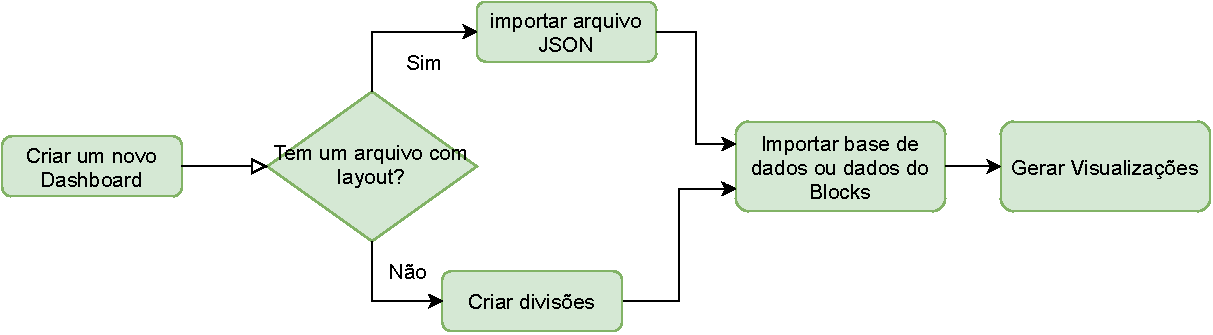
\includegraphics[scale=1]{figures/Diagrama de fluxo tcc.pdf}
	\end{center}
	\legend{Fonte: O autor}
\end{figure}

\section{Arquitetura}
A Arquitetura organizacional do projeto foi definida como um MVC (\textit{Model, View, Controller}) definido por \cite{deacon2009model}, como um modelo com três camadas: modelo, responsável pela estrutura de dados, visão, a interface gráfica disponibilizada para o usuário, e o controlador, responsável por conter a regra de negócio da aplicação. A arquitetura foi desenvolvida em um modelo incremental com constantes reuniões para discussão para propostas de melhorias e novas funcionalidades na ferramenta. 

No desenvolvimento foi selecionada a linguagem de programação \textit{javacript} ou \textit{Ecmascript 6} aproveitando de seus novos recursos como \textit{Arrow Functions}, \textit{Array Destructuring} e classes, em conjunto com o \textit{framework} \textit{electron} \cite{electron} para criação de uma aplicação \textit{desktop} compatível com sistemas operacionais \textit{Windows}, Linux e Mac, além disso os gráficos disponíveis foram implementados no Vistechlib uma biblioteca de módulos reutilizáveis de visualização da informação \cite{Vistechlib}. Bem como, foi implementado um modulo de leitura da bases de dados para converter objetos CSV, JSON, TSV e tratar os dados categóricos e contínuos, e adicioná-los na ferramenta para filtros e seleções, também foi criada uma estrutura de comunicação por \textit{socket} para comunicar a aplicação desenvolvida com a ferramenta de geração de dados \textit{Blocks} \cite{blocks} que requisita esses dados para gerar visualizações .


A \autoref{mvc_app} contém uma representação do fluxo de troca de informações na ferramenta e sua estrutura MVC mencionada anteriormente e suas principais atividades de cada camada. No \textsf{model} como mostrado na \autoref{mvc_app} contém dois principais módulos, o de "leitura de dados e conversão" onde é feita a leitura da base de dados e sumarizado para ferramenta para serem interpretados pelas visualizações e interfaces, bem como o módulo de estrutura de  \textsf{layout} onde pode ser carregado um arquivo JSON que contém as posições, divisões, tamanhos das estruturas de tela e visualizações que podem ser importadas e exportadas para utilizações posteriores.

\begin{figure}
	\caption{\label{mvc_app}Arquitetura MVC implementada na ferramenta desenvolvida, seus principais componentes, trocas de informações disponíveis nos módulos do sistema. A camada  \textsf{model} onde contém as estruturas de dados, o \textsf{controller} com as regras de criações de visualizações e criação de  \textsf{layout} de tela, e a  \textsf{view} com as interfaces para o usuário}
	\begin{center}
	    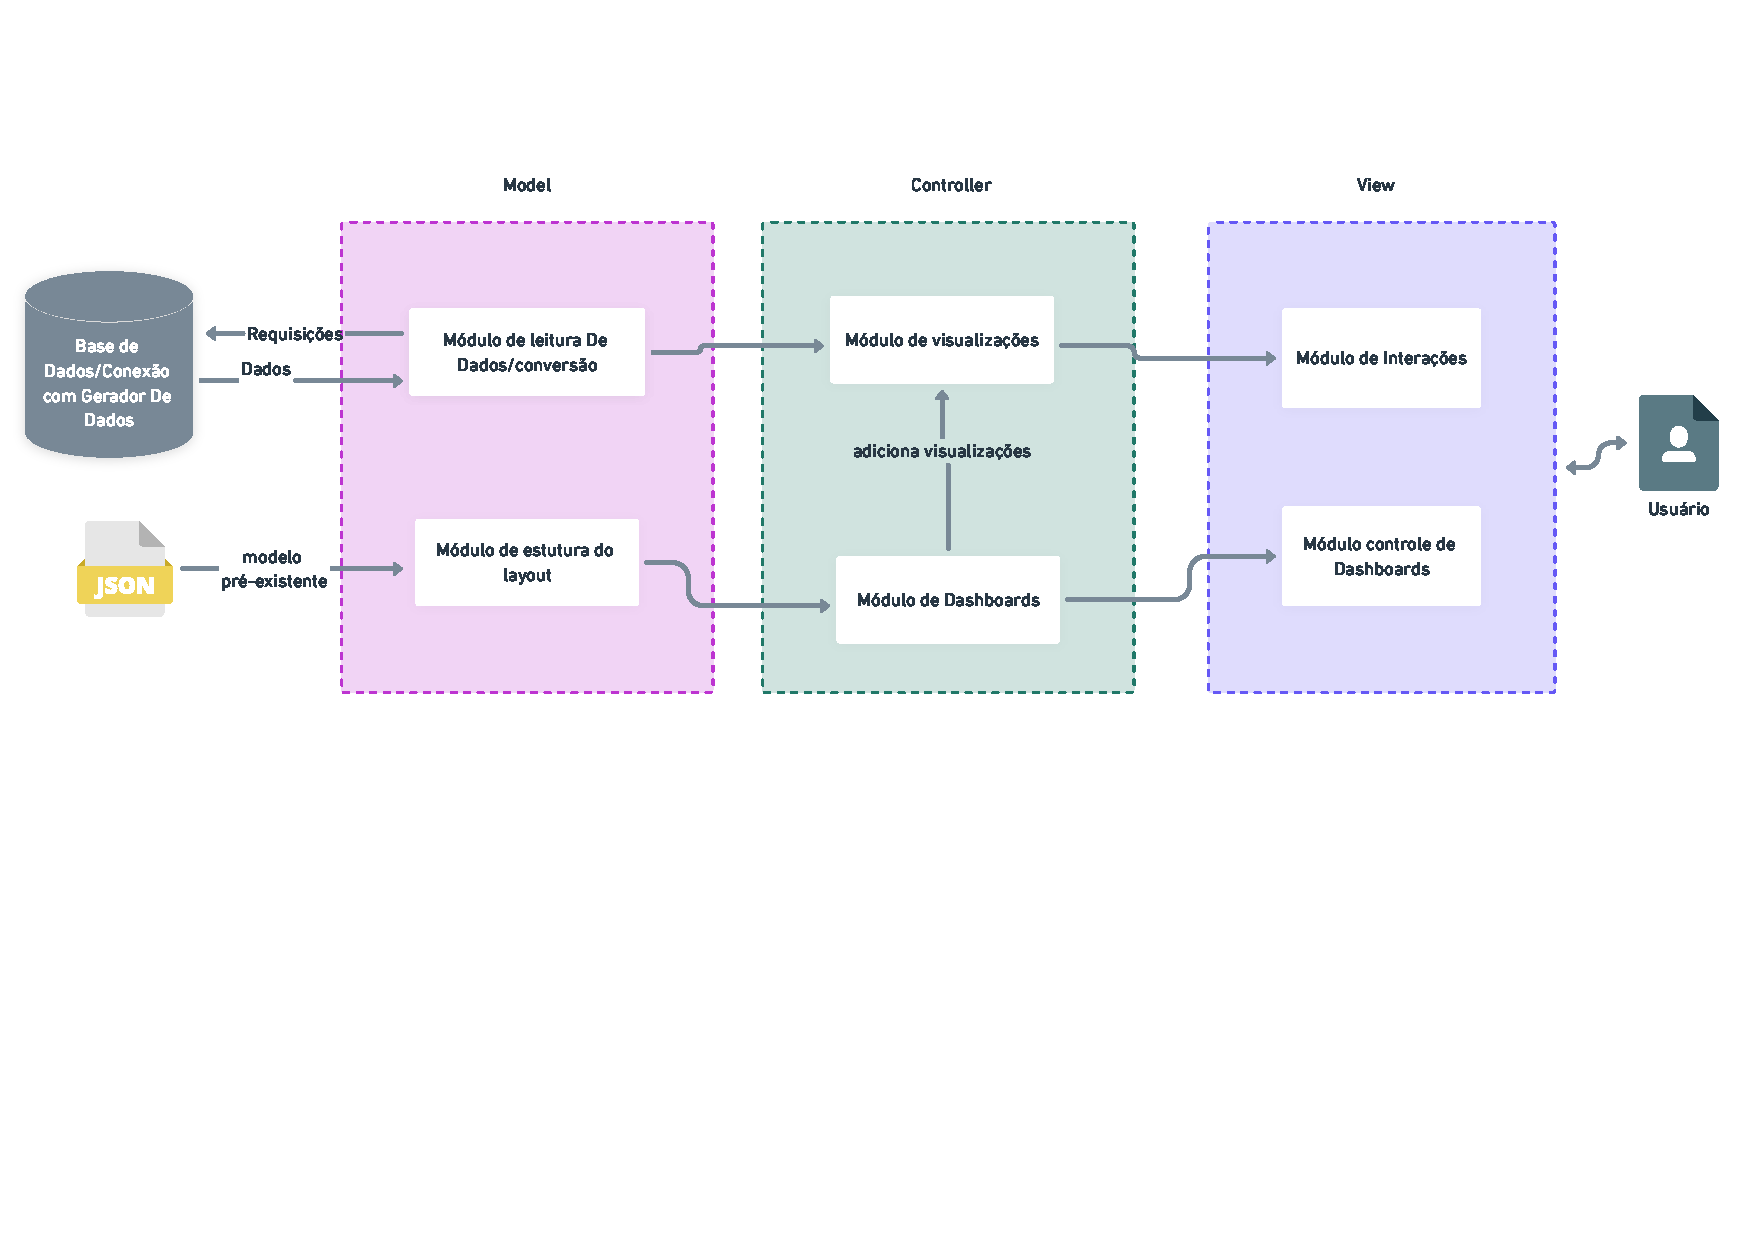
\includegraphics[width=40pc,trim={0 260 0 0}]{figures/mvc_diagrama.pdf}}
	\end{center}
	\legend{Fonte: O autor}
\end{figure}


Já no \textit{controller} podemos ver os seguintes módulos que contém a regra de negócio se comunicando com os \textit{models} e  \textit{view} que são respectivamente o módulo de visualizações responsável por criar, customizar, deletar e oferecer as interações das visualizações e o módulo de \textit{dashboards} que tem com finalidade a criação e customização das subdivisões para criação dos \textit{dashboards}.

Na \textit{view} contém o módulo de interações e o módulo controle de \textit{dashboards}, que são as interfaces gráficas onde o usuário realiza por meio do mouse suas interações para customizar gráficos e subdivisões de telas.


\section{Diagrama de casos de uso}
Nesta seção serão abordados os casos de uso da aplicação, os fluxos e as principais utilizações pelo usuário da ferramenta.

As possibilidades de uso da ferramenta pelo usuário estão descritas no diagrama de casos de uso na \autoref{casos_de_uso_uml}, onde nessa figura estão descritas as funcionalidades disponíveis da ferramenta.

O diagrama de casos de uso na \autoref{casos_de_uso_uml} ilustra os possíveis fluxos de criação de \textit{dashboard}, desde a criação do layout até a interação nas visualizações disponíveis ou, caso seja desejo do usuário, a criação de apenas uma visualização e exploração por meio de interações, bem como o carregamento de um \textit{dashboard} pré-existente gerado pela ferramenta também pode ser realizado.

\begin{figure}
	\caption{\label{casos_de_uso_uml}Diagrama de casos de uso da ferramenta para criação de um novo \textit{dashboard} ou visualização }
	\begin{center}
	    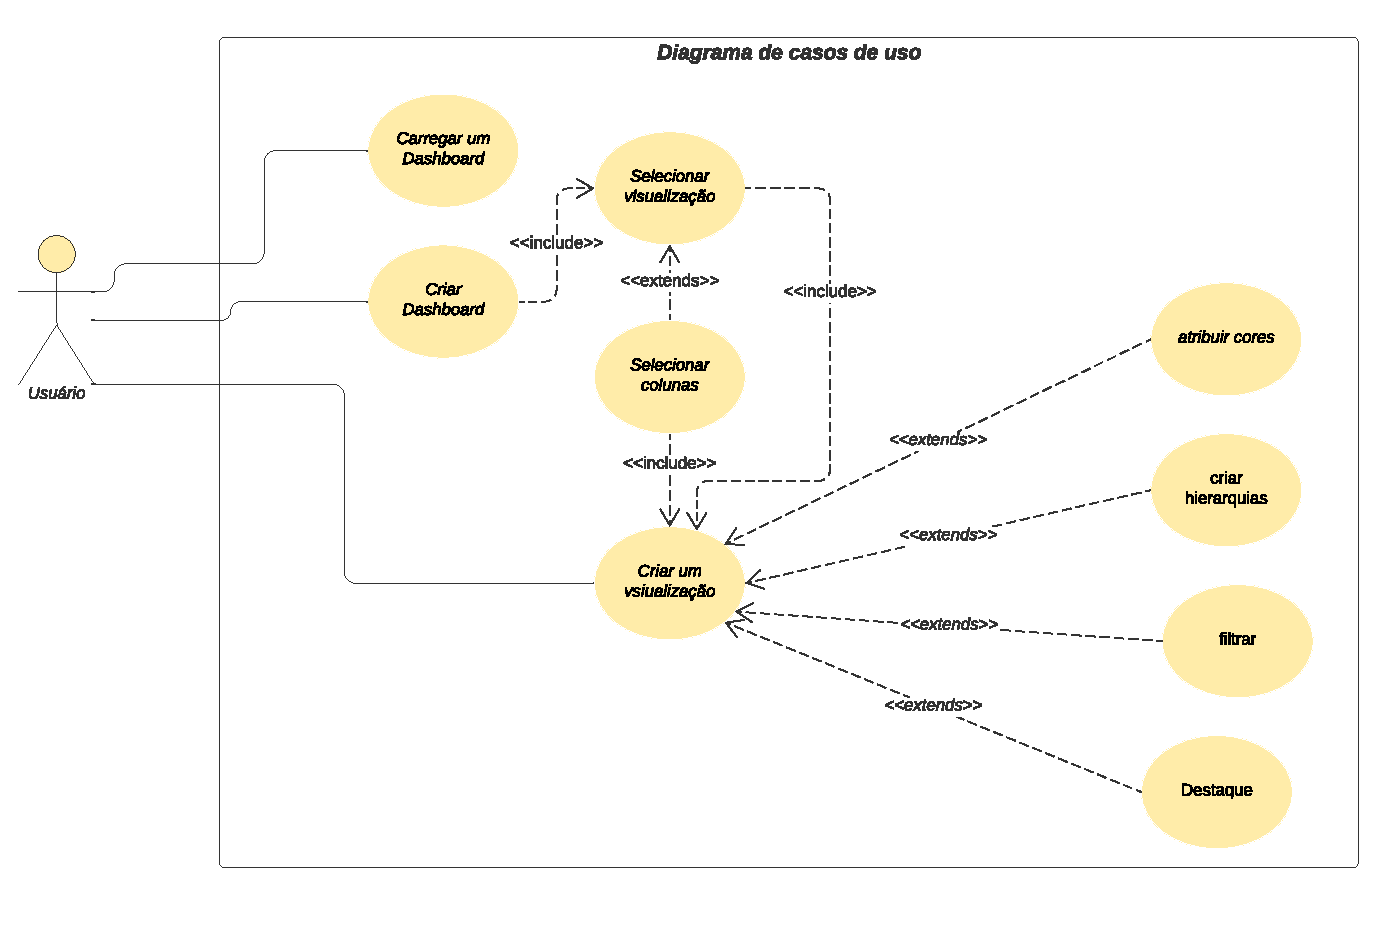
\includegraphics[width=35pc,size=1]{figures/Diagrama de casos de uso.pdf}
	\end{center}
	\legend{Fonte: O autor}
\end{figure}

\section{Diagrama de classes}
O diagrama de classes demonstrado na \autoref{classe_uml} exemplifica a estrutura de classes resumida para a geração dos gráficos. A classe abstrata \textit{Visualization}  possui os métodos e atributos onde cada subclasse de gráfico irá sobrescrever e herdar os comportamentos da classe abstrata. Os principais métodos disponíveis na classe abstrata compartilhada com as subclasses são  \textit{data()},  \textit{redraw()},  \textit{resize()}, e \textit{bindMouseEvents()}, esses métodos respectivamente são responsáveis por \textit{data()} processar e atribuir os dados para um objeto, \textit{redraw()} é o método onde contém a lógica de desenho para cada gráfico utilizando d3.js, o método \textit{resize()} tem a responsabilidade de redimensionar o tamanho do gráfico conforme o tamanho disponível em tela ou subdivisão de tela, já o método \textit{bindMouseEvents()} tem como objetivo permitir a interação com o mouse nos componentes equivalentes aos dados.

A segunda parte da \autoref{classe_uml} demonstra o controlador de interações para cada visualização seguindo o padrão clássico \textit{strategy} catalogado no trabalho de \cite{gamma1995design}. A classe \textit{Interaction Manenger} tem o objetivo de fornecer os métodos para que as interações possam ser selecionadas \textit{select()}, desselecionadas \textit{unselected()}, e desativadas \textit{disable()}, a importância desse método é permitir que, em tempo de execução, as interações sejam trocadas rapidamente e não gerem conflitos para o usuário final.

O Diagrama na \autoref{classe_uml_layout}  representa as classes responsáveis pela geração do layout customizável para criação de novas divisões, onde serão organizados as visualizações, criando um \textit{dashboard} ao final, essa geração pode ser feita em tempo real com cliques no \textit{mouse} ou realizada com base em um arquivo JSON. No diagrama de classe da \autoref{classe_uml_layout} podemos ver a relação de composição do layout dinâmico de \textit{dasboards} onde temos as classes \textit{PartitionLayout} que contém os elementos redimensionáveis e que podem ser divididos, a classe \textit{Partion} onde é criada uma partição horizontal ou vertical, criando uma nova divisão no HTML, e a classe \textit{Divisor} que representa a linha divisória e redimensionável do layout com uma composição da classe \textit{PlaceHolderDivisor} para verificar cálculos e mostrar a interação de redimensionamento das divisões na tela.


\begin{figure}
	\caption{\label{classe_uml}Diagrama de classes para a geração das visualizações e seus métodos em conjunto com as classes para controlar as interações  }
	\begin{center}
	    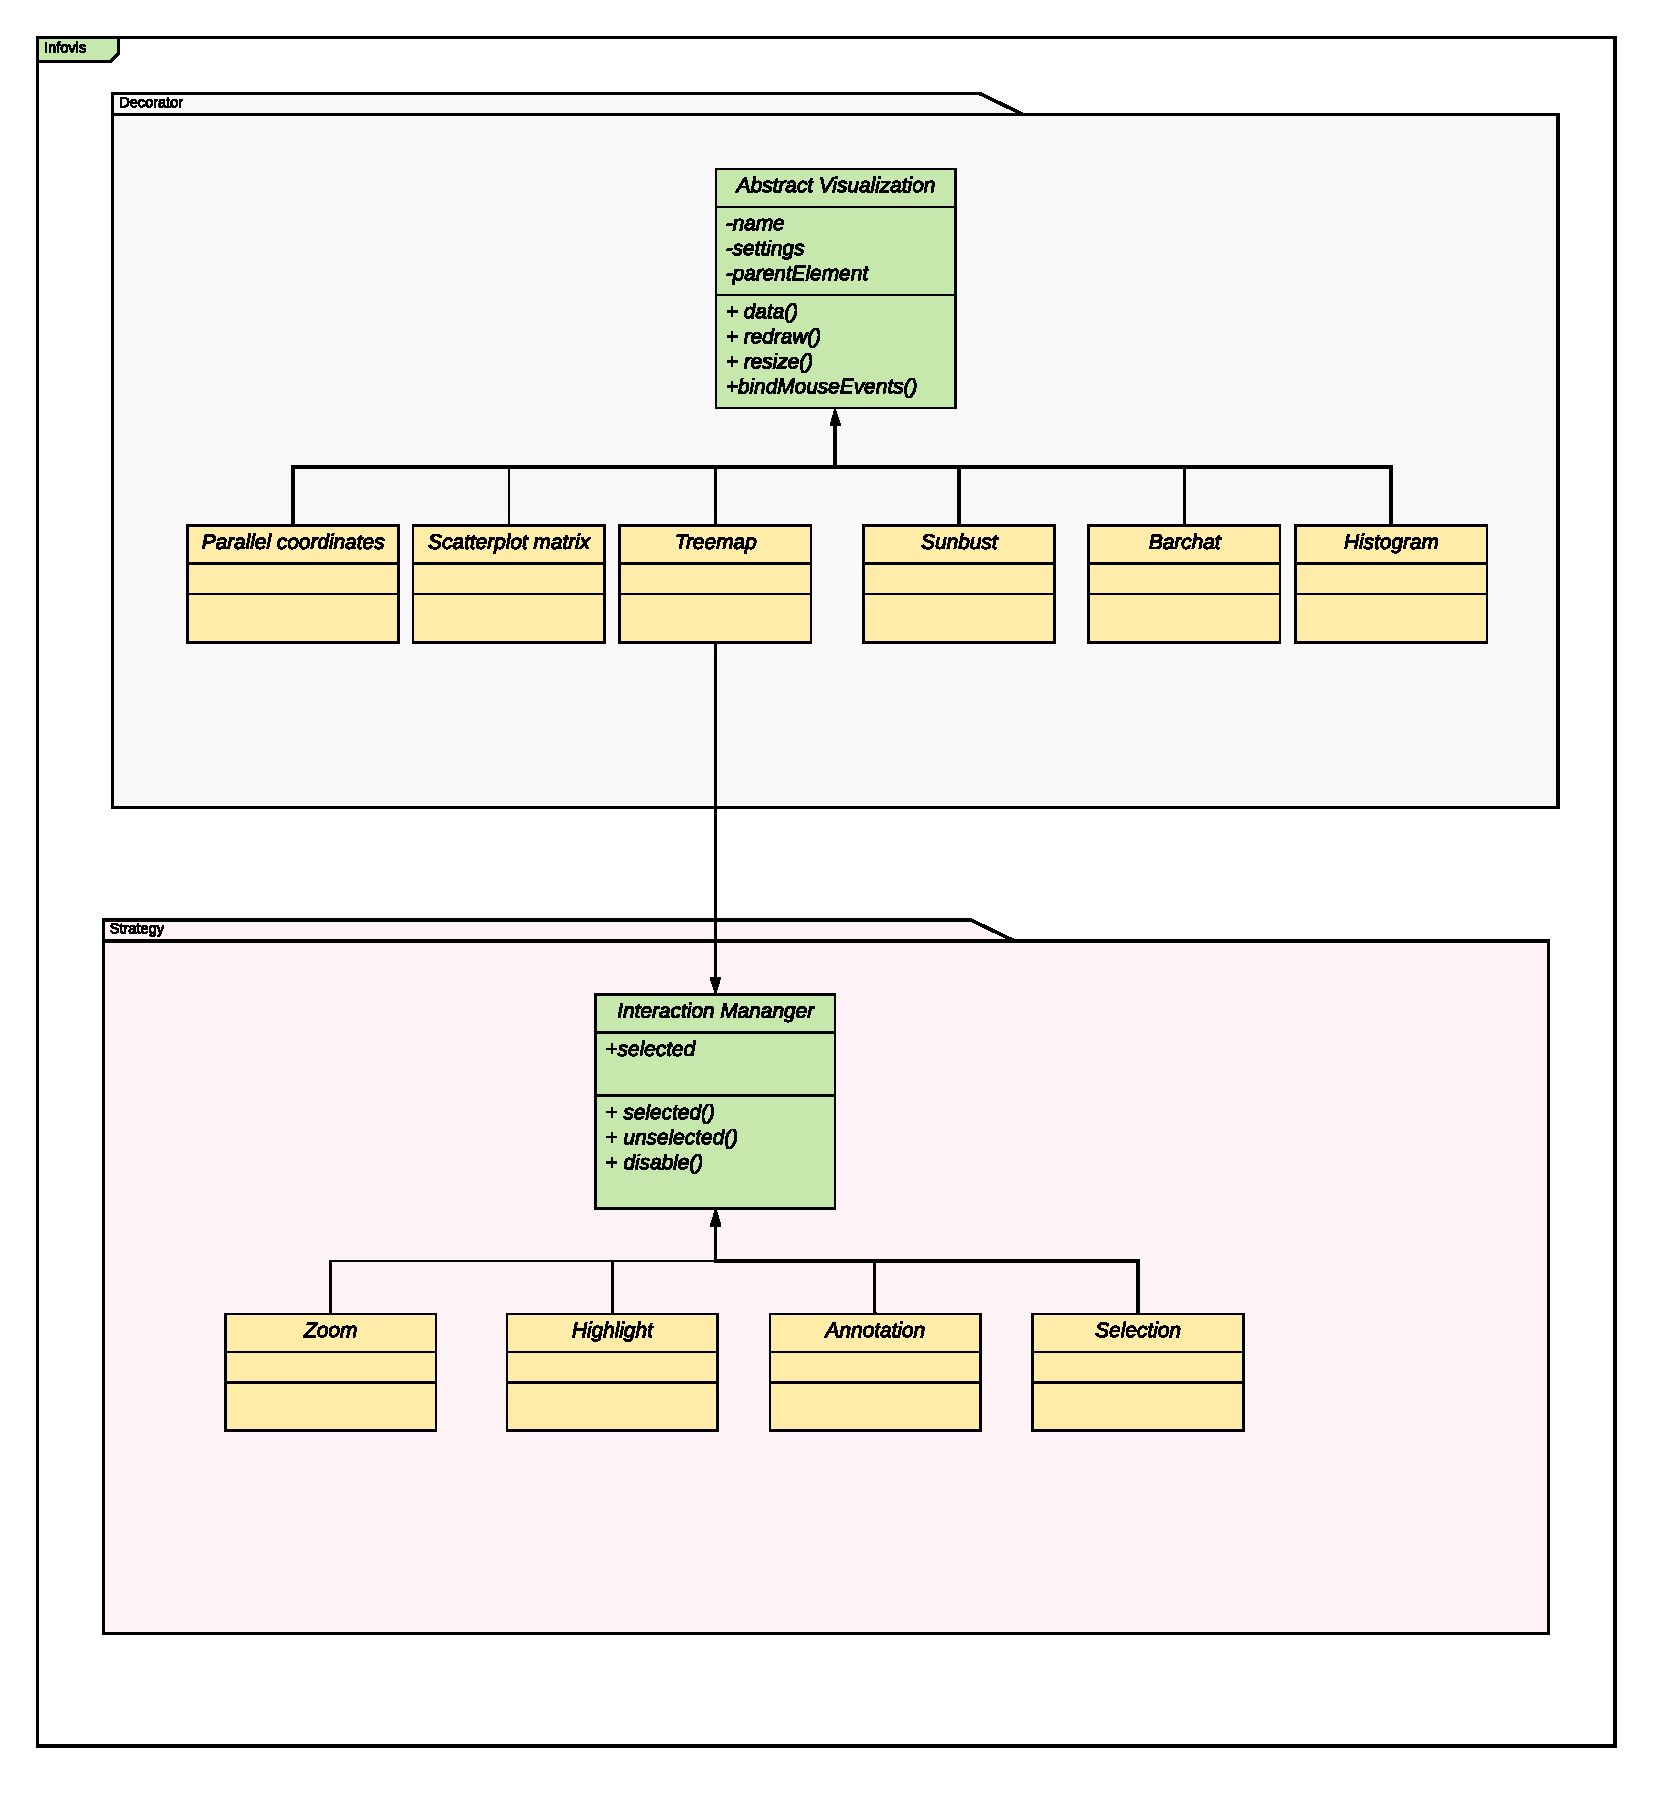
\includegraphics[width=35pc,height=35pc]{figures/visApplication uml(1).pdf}
	\end{center}
	\legend{Fonte: O autor}
\end{figure}

\begin{figure}
	\caption{\label{classe_uml_layout}Diagrama de classes para a geração dos layout interativos para criação dos \textit{dashboards} onde as classes \textit{PartitionLayout}, \textit{Partion}, \textit{Divisor}, \textit{PlaceHolderDivisor}, tem uma relação de composição na qual são dependentes para existirem }
	\begin{center}
	    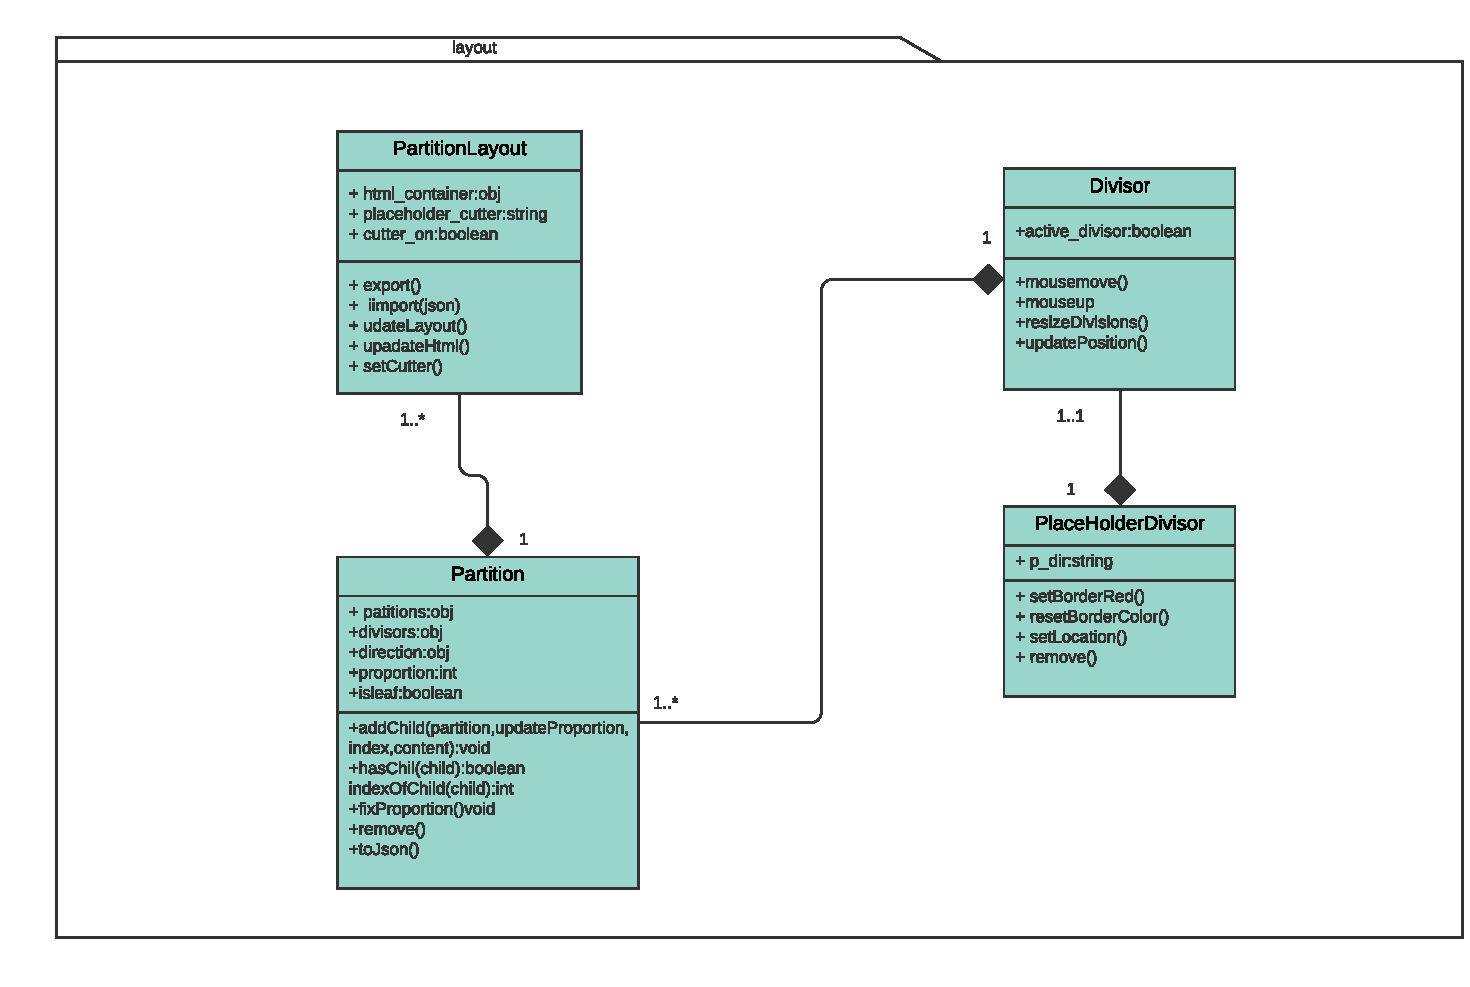
\includegraphics[width=40pc,height=30pc]{figures/Diagrama layout parrtition.pdf}
	\end{center}
	\legend{Fonte: O autor}
\end{figure}




\section{Protótipo}
O Protótipo é responsável pela construção das visualizações da dados, assim como pela criação dos layouts de  \textit{dashboards}, sendo assim é passível utilizar visualizações únicas seguindo o \textit{pipeline} clássico de visualização de dados, transformando os dados em dados tabulares e convertendo as estruturas em variáveis visuais que compõem uma visualização completa com interações fornecidas ao usuário final.  

Nas funcionalidades do protótipo, um dos principais destaques é a criação de \textit{dashboards} dinâmicos provenientes de divisões horizontais e verticais onde, a tela pode ser subdividida em uma dessas divisões, pode ser selecionada qual visualização ficará nesse local dependendo da vontade do usuário.
As interações ocorrem por meio do mouse, onde é possível subdividir a tela, a partir da posições do mouse, bem com, também é possível carregar um arquivo JSON com o formato que foi gerado pela ferramenta com um layout de tela já pré-existente.  

\subsection{Criação de \textit{dasbboards} flexíveis} 

A criação dos \textit{layouts} das partições,para a geração das teças dos \textit{dashboards} são feitas com base no \textit{layout flex-box} definido em \cite{w3c}
é um modulo de criação de layout flexível tornando mais fácil  cria uma estrutura responsiva sem utilizar os \textit{display} flutuante o definir o posicionamento.

Para a criação da divisão de telas do \textit{dasbboards} foi desenvolvido um padrão de objeto JSON para quando for realizado a leitura pelos módulos de geração de \textit{layout} ,o protótipo gerar as divisões de telas somente ou as divisões de telas com as visualizações já presentes. Abaixo segue um trecho resumido de exemplo do objeto JSON para criação das divisões de telas. 

\begin{minted}{json}

{
        "id": "000001",
        "direction": "column",
        "proportion": 1
        "isLeaf": false,
        "children": [
            {"id":"..."},
            {"id":"..."},
        ],
        "content": {
            "vis_name": ""
        }
        
}
\end{minted}

Os seguintes atributos descrevem  o arquivo JSON para a criação de \textit{dashboards} (\textit{id}) indicação de referencia para o HTML,  (\textit{parent}), a partição para pai apenas se for root não e refeneciado, (\textit{proportion}) a proporção do da partição em relação ao total variando em numero entre 0 e 1, (\textit{isLeaf}) boleano se é folha ou não indica se é ultimo no da árvore de estrutura, (\textit{html}) referencia do elemento HTML,(\textit{content}) que representa o conteúdo contido nessa divisão , e o atributo (\textit{vis-name}) contém o nome do da visualização que será gerada pelo protótipo.

Outro atributo importante é o (\textit{direction}) a direção que pode ser referenciada como linha \textit{row} linha os elementos divisões horizontais ou colunas \textit{collun} para divisões verticais. O atributo (\textit{children}) tem como objetivo criar as subdivisões tanto verticais quanto horizontais, adicionando um novo objeto com todos os atributos da partições e dentro dessas partições podem conter o atributo \textit{children} com novas hierarquias de subdivisões. segue a baixo alguns trechos de código e das partições e suas respectivas telas geradas pela aplicação. Para realizar a importação das visualizações se a partição for um nó folha podemos adicionar um conteúdo HTML por padrão e colocado um \textit{button} HTML para adicionar uma nova visualização ou no caso já esteja adicionado um conteúdo e selecionada o nome da visualização para ser gerada na biblioteca de gráficos quando importado o arquivo JSON.

\begin{itemize}
    \item exemplo de \textit{layout horizontal} com hierarquias internas:
    
    No trecho de código a baixo podemos ver um JSON resumido das partições e na \autoref{jsonLayout} o resultado demonstrado na tela. Pode ser visto no arquivo JSON , três objetos dentro no atributo \textit{children} com as direções atribuídas como linhas formado divisões horizontais que são renderizadas na tela \autoref{jsonLayout}.
     
    
\begin{minted}{json}
{
  "id": "000001",
  "direction": "column",
  "proportion": 1,
  "isLeaf": false,
  "children": [
    {
      "id": "yPUMKeqy","direction": "row" ,...  "content": { "vis_name": ""}
    },
    {
      "id": "WoWL6gfs","direction": "row" ,... "content": { "vis_name": ""}
    },
    {
      "id": "Qpi3CeCZ","direction": "row" ,... "content": { "vis_name": ""}
    }
  ]
  
}

\end{minted}

\begin{figure}[!ht]
	\caption{\label{jsonLayout} tela com divisões horizontais renderizadas pelo arquivo JSON  }
	\begin{center}
	    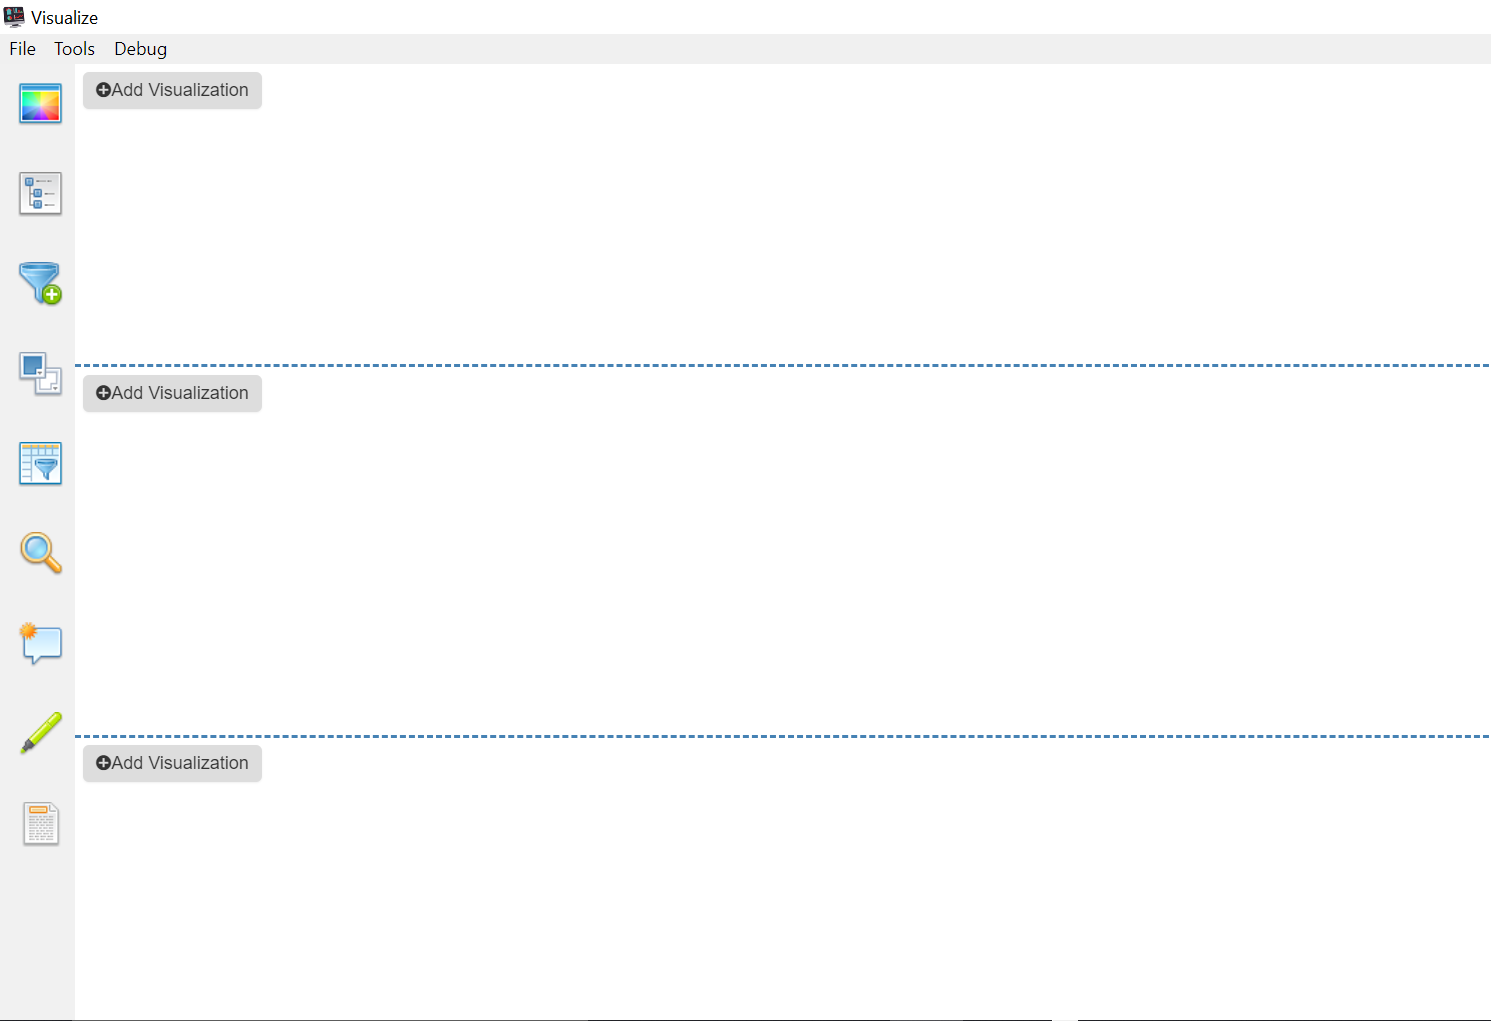
\includegraphics[width=20pc]{figures/layout1.PNG}
	\end{center}
	\legend{Fonte: O autor}
\end{figure}

    \item exemplo com divisões verticais e horizontais com hierarquias internas:
      No trecho de código a exemplificado baixo podemos ver o código resumido das partições e na \autoref{jsonLayout2} o resultado demonstrado em tela. 
      Pode ser visto no arquivo JSON , três objetos no atributo \textit{children} formando divisões verticais, e no ultimo objeto contém um hierarquia onde no tributo \textit{children} contém mais 3 subdivisões porém nesse caso horizontal.

\begin{minted}{json}
{
    "id": "9DQKqoHJ",
    "direction": "row",
    "proportion": 1,
    "isLeaf": false,
    "children": [
      { "id": "JExJIFTB",... "direction":"column",},
      {"id": "av7uH3nJ",... "direction": "column",},
      {"id": "Qi7CvVct",... "direction": "column",
        "children": [
          {"id": "NVIkahpx",... "direction": "row",},
          {"id": "7IbAmqiH",... "direction": "row",},
          {"id": "d8vOojb8",... "direction": "row",}
        ]
      }
    ]
}

\end{minted}
\begin{figure}[!ht]
	\caption{\label{jsonLayout2} tela com divisões horizontais proveniente do arquivo JSON  }
	\begin{center}
	    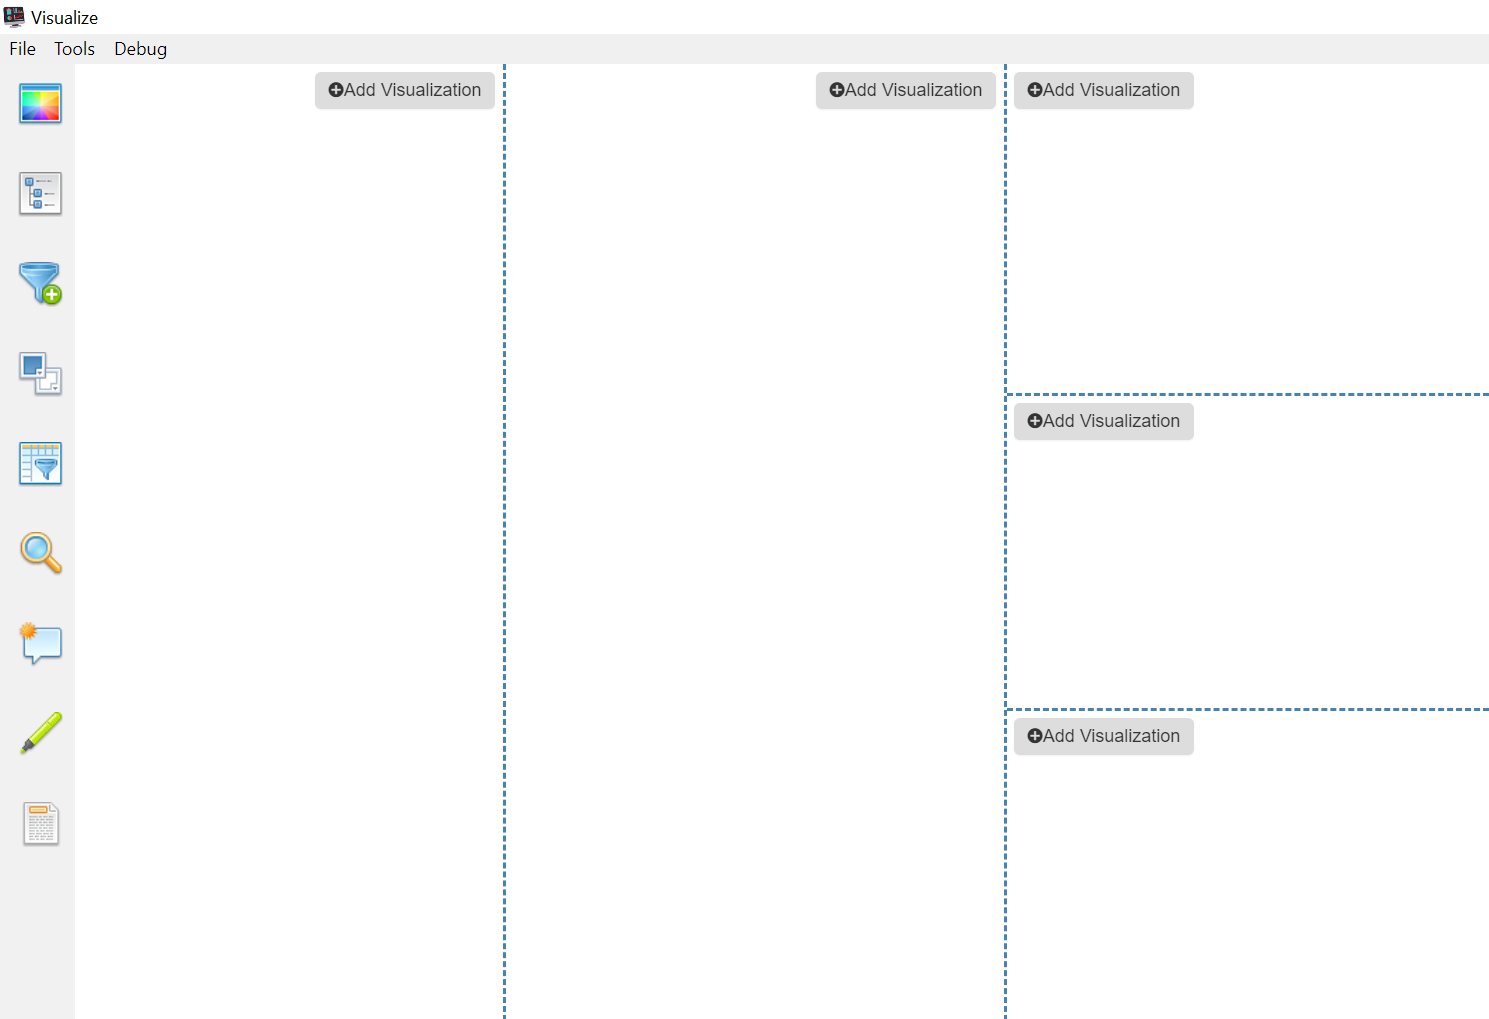
\includegraphics[width=20pc]{figures/layout2.PNG}
	\end{center}
	\legend{Fonte: O autor}
\end{figure}
    
    
    \item exemplo de \textit{dashboard} com divisões horizontais e verticais com visualizações criando  um \textit{dasboard}:
    
    No terceiro trecho de código a exemplificado podemos ver o código resumido das partições e na \autoref{jsonLayout3} o resultado renderizado em tela.
    o no código do arquivo JSON temos 3 partições, uma horizontal com o conteúdo uma visualização de coordenadas paralelas, e duas partições horizontais, a primeira com o conteúdo de um \textit{treemap}, e a segunda o gráfico de  \textit{Circle packing} .
    
    
\begin{minted}{json}
{
  "id": "000001",
  "direction": "column",
  "proportion": 1,
  "isLeaf": false,
  "children": [
    {
      "id": "eGZUMUu3","direction": "row","proportion": 0.32,"isLeaf": true,
      "content": { 
        "vis_name": "ParallelCoordinates"
        }
    },
    {"id": "E1zTNOy8","direction": "row","proportion": 0.67,"isLeaf": false,
      "children": [
        {"id": "0YBMY2aW","direction": "column",...,
        "content": { 
            "vis_name": "Treemap"
        }},
        {" id": "GWYxFgAY","direction": "column",...,
        "content": { 
            "vis_name": "CirclePacking"
        }}
      ]}
  ]
}



\end{minted}
    
\begin{minted}
{
  "id": "E1zTNOy8",
  "direction": "row",
  "proportion": 0.6786833855799372,
  "isLeaf": false,
  "children": [
    {
      "id": "0YBMY2aW",
      "direction": "column",
      "proportion": 0.4944972681398257,
      "isLeaf": true
    },
    {
      "id": "GWYxFgAY",
      "direction": "column",
      "proportion": 0.5055027318601744,
      "isLeaf": true
    }
  ]
}

\end{minted}

\begin{figure}[ht]
	\caption{\label{jsonLayout3} tela com divisões e visualizações proveniente do arquivo JSON}
	\begin{center}
	    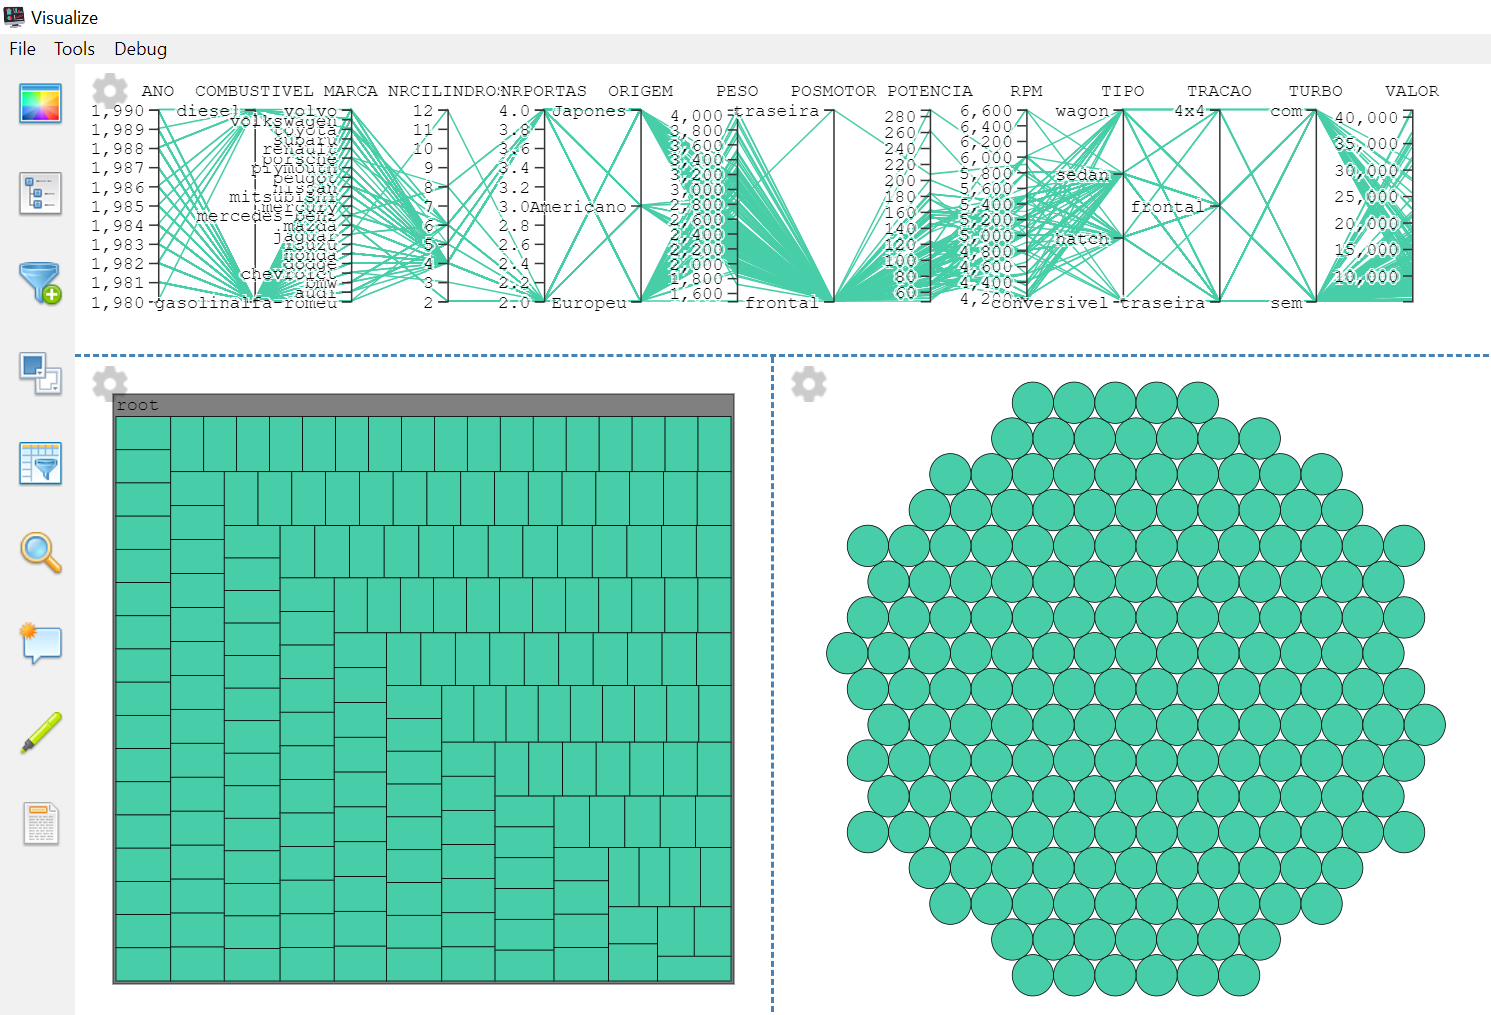
\includegraphics[width=20pc]{figures/layout3.PNG}
	\end{center}
	\legend{Fonte: O autor}
\end{figure}


\end{itemize}


\subsection{Visualizações Disponíveis}
Nesta seção serão apresentas as visualizações disponíveis no protótipo desenvolvido, diversas visualizações foram implementadas com diferentes objetivos, como visualizações multidimensionais, unidimensionais, hierárquicas, árvores, e visualizações de linha. As visualizações disponíveis são \textit{Beeswarm Plot}, textit{Circle Packing}, \textit{Coordenadas Paralelas}, Gráfico de Barras,\textit{Histograma}, Matriz de \textit{Scatter Plot},\textit{Parallel Bundling}, \textit{Sunburst} e \textit{Treemap}, abordadas abaixo: 

\begin{itemize}
    \item  \textbf{\textit{Beeswarm Plot}}:
    Pode ser descrito como uma gráfico de dispersão uni-dimensional semelhante a um enxame de abelhas onde os pontos não se sobrepõem e cada item representa uma posição em relação ao eixo de valor, além do posicionamento, os pontos podem conter um valor atribuído a uma cor, como exemplo \autoref{fig_beeswarm}.
    
    \begin{figure}
	\caption{\label{fig_beeswarm} Gráfico \textit{Beeswarmplot} desenvolvido na aplicação}
	\begin{center}
	    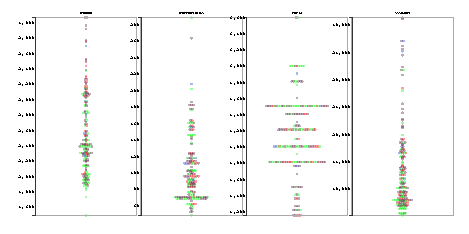
\includegraphics[width=40pc,size=1]{figures/bewarmplot.pdf}
	\end{center}
	\legend{Fonte: O autor}
\end{figure}
    
    \item  \textbf{\textit{Circle Packing}}:
    Pode ser descrito como uma técnica de visualização de empacotamento de círculos na qual, pode ou não existir hierarquias. Aos itens podem ser atribuídas cores, enquanto que os tamanhos podem codificar uma variável da base de dados, como por exemplo, na \autoref{cirlces} onde são ilustrados hierarquias, cores e tamanhos representando valores da base de dados. 
    
\begin{figure}
	\caption{\label{cirlces}Gráfico de \textit{Circle Packing}  gerado pela ferramenta}
	\begin{center}
	    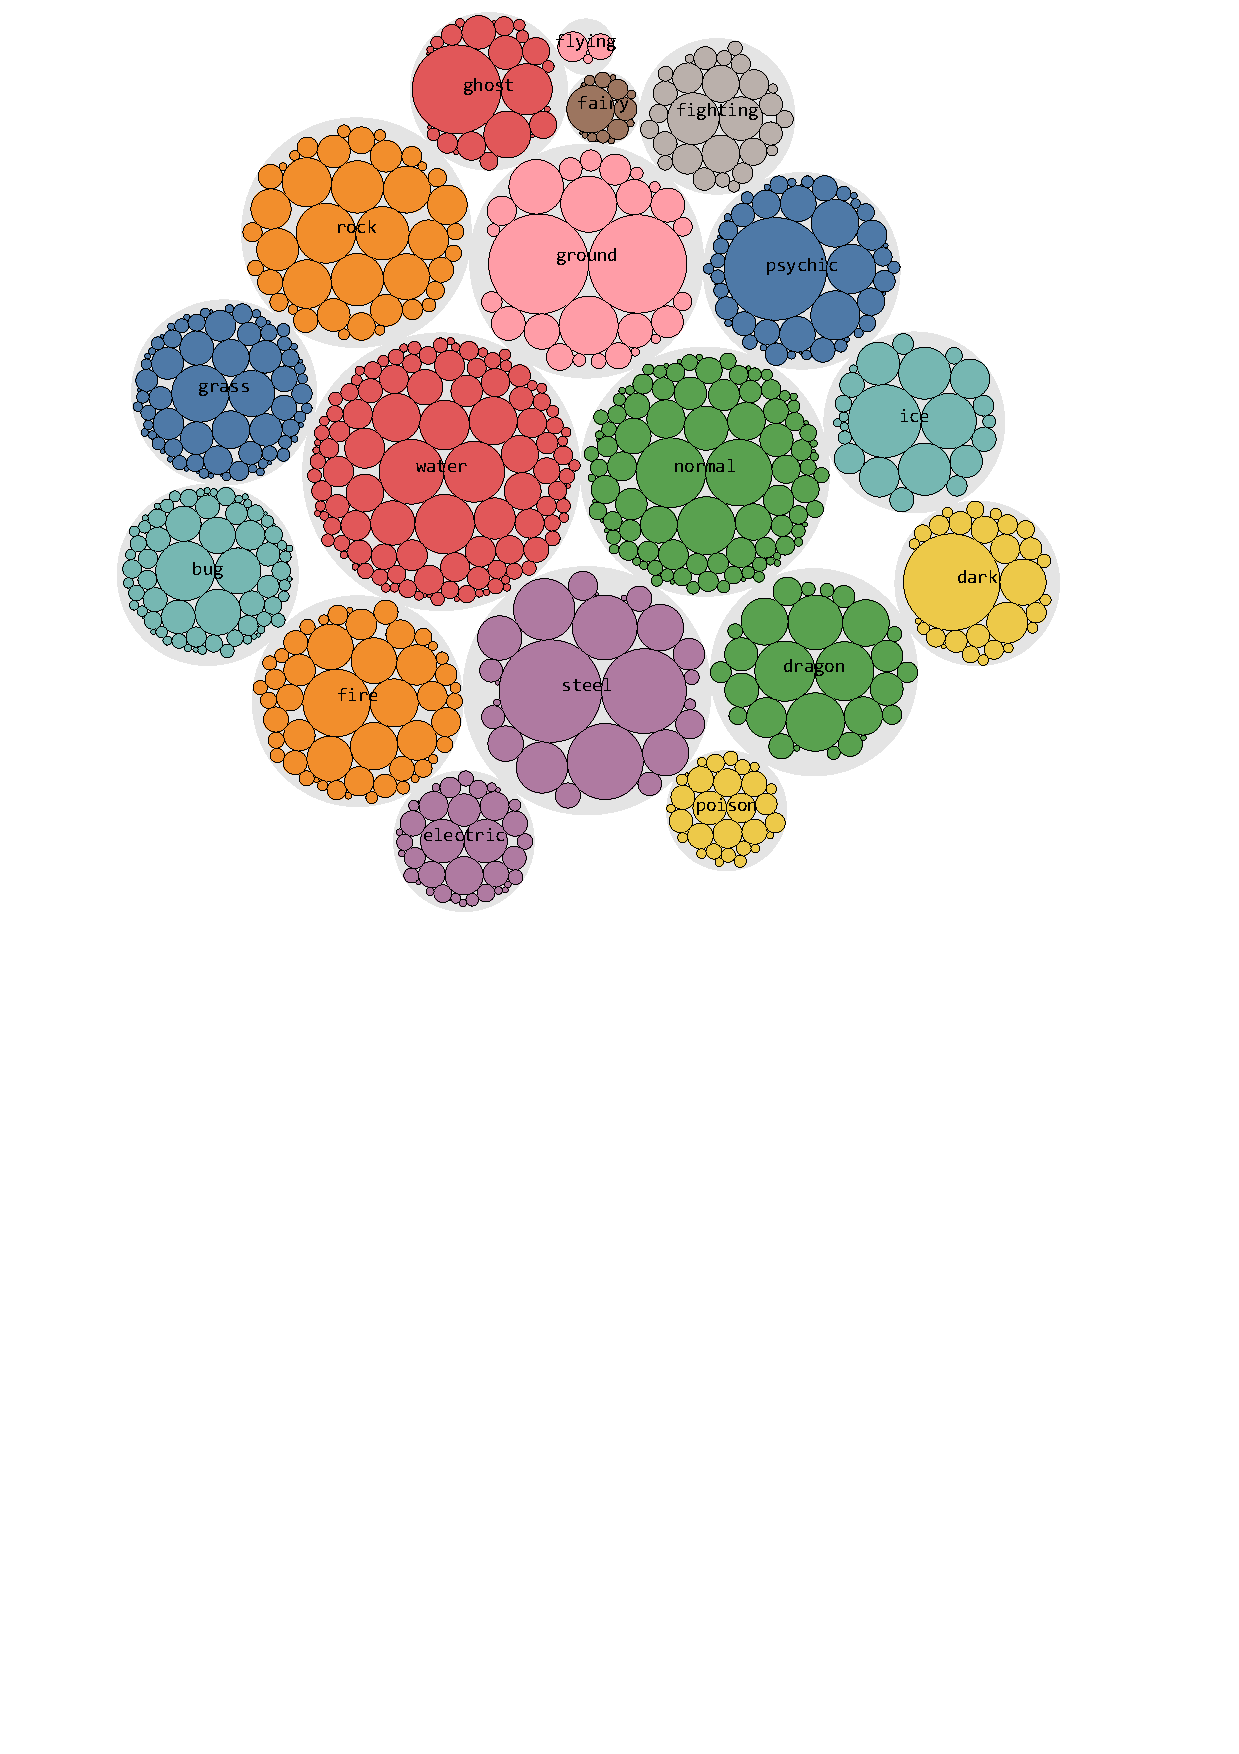
\includegraphics[width=40pc,size=1,trim={1cm 140mm, 1.5cm 0mm},clip]{figures/circle_packing.pdf}
	\end{center}
	\legend{Fonte: O autor}
\end{figure}
    
    
    
    \item   \textbf{Coordenadas Paralelas}:
    A técnica de coordenadas paralelas ilustrada na \autoref{paralle_Cordinates}, desenvolvida por \cite{inselberg1985plane} apresenta uma visualização para dados multidimensionais, onde eixos paralelos verticais ou horizontais são exibidos na tela para representar as dimensões e linha ou polígonos atravessam esses eixos em uma posição delimitando os valores dos registros nessa dimensão. Eixos podem ser reordenados e as cores também podem representar uma dimensão.

    \begin{figure}
	\caption{\label{paralle_Cordinates}Gráfico de coordenadas paralelas gerado pela ferramenta}
	\begin{center}
	    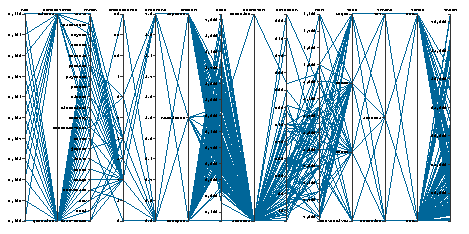
\includegraphics[width=40pc,height=25pc,size=1]{figures/parallel.pdf}
	\end{center}
	\legend{Fonte: O autor}
\end{figure}
    
    \item  \textbf{Gráfico de Barras}:
    O gráfico de barras verticais pode ser descrito como um conjunto de barras retangulares onde o cumprimento é proporcional aos valores que estão sendo representados. Os eixos demonstram o que está sendo comparado nas barras, sendo que a ilustração de um gráfico de barras gerado pela aplicação pode ser visualizado na \autoref{barchart}
    
\begin{figure}
	\caption{\label{barchart}Gráfico de Barras gerado pela ferramenta}
	\begin{center}
	    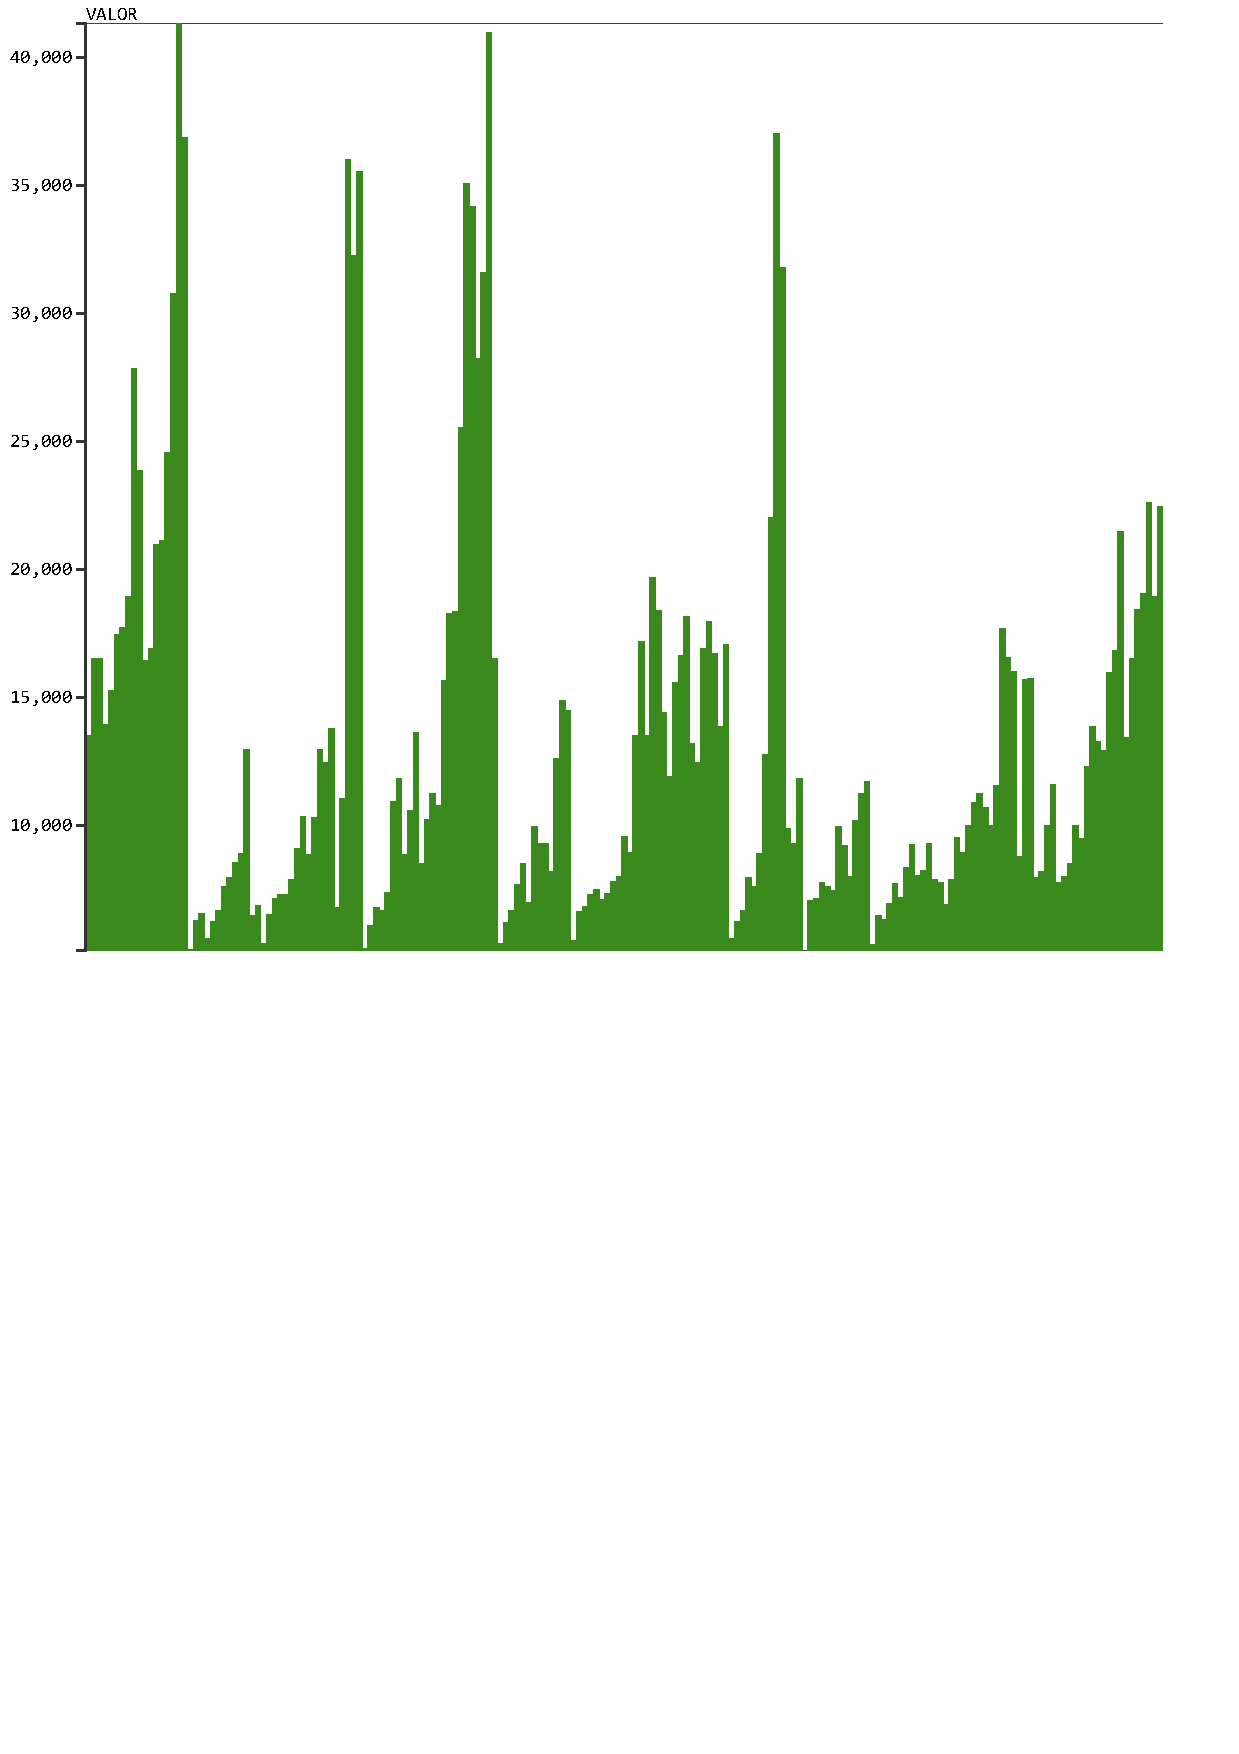
\includegraphics[width=40pc,size=1,trim={1cm 140mm, 1.5cm 50mm},clip]{figures/barchar.pdf}
	\end{center}
	\legend{Fonte: O autor}
\end{figure}
    
    
    \item  \textbf{Histograma}:
    O gráfico de histograma é composto por barras sequenciais em sua versão implementada na ferramenta disponível na \autoref{fig_histograma} onde representam a distribuição de frequência, no histograma cada barra representa um registro ou dado, bem como a altura representa o valor desse registro utilizado para dados contínuos, o histograma tem como objetivo observar a distribuição da amostragem selecionada.
    
\begin{figure}
	\caption{\label{fig_histograma} Exemplo do histograma desenvolvido na ferramenta}
	\begin{center}
	    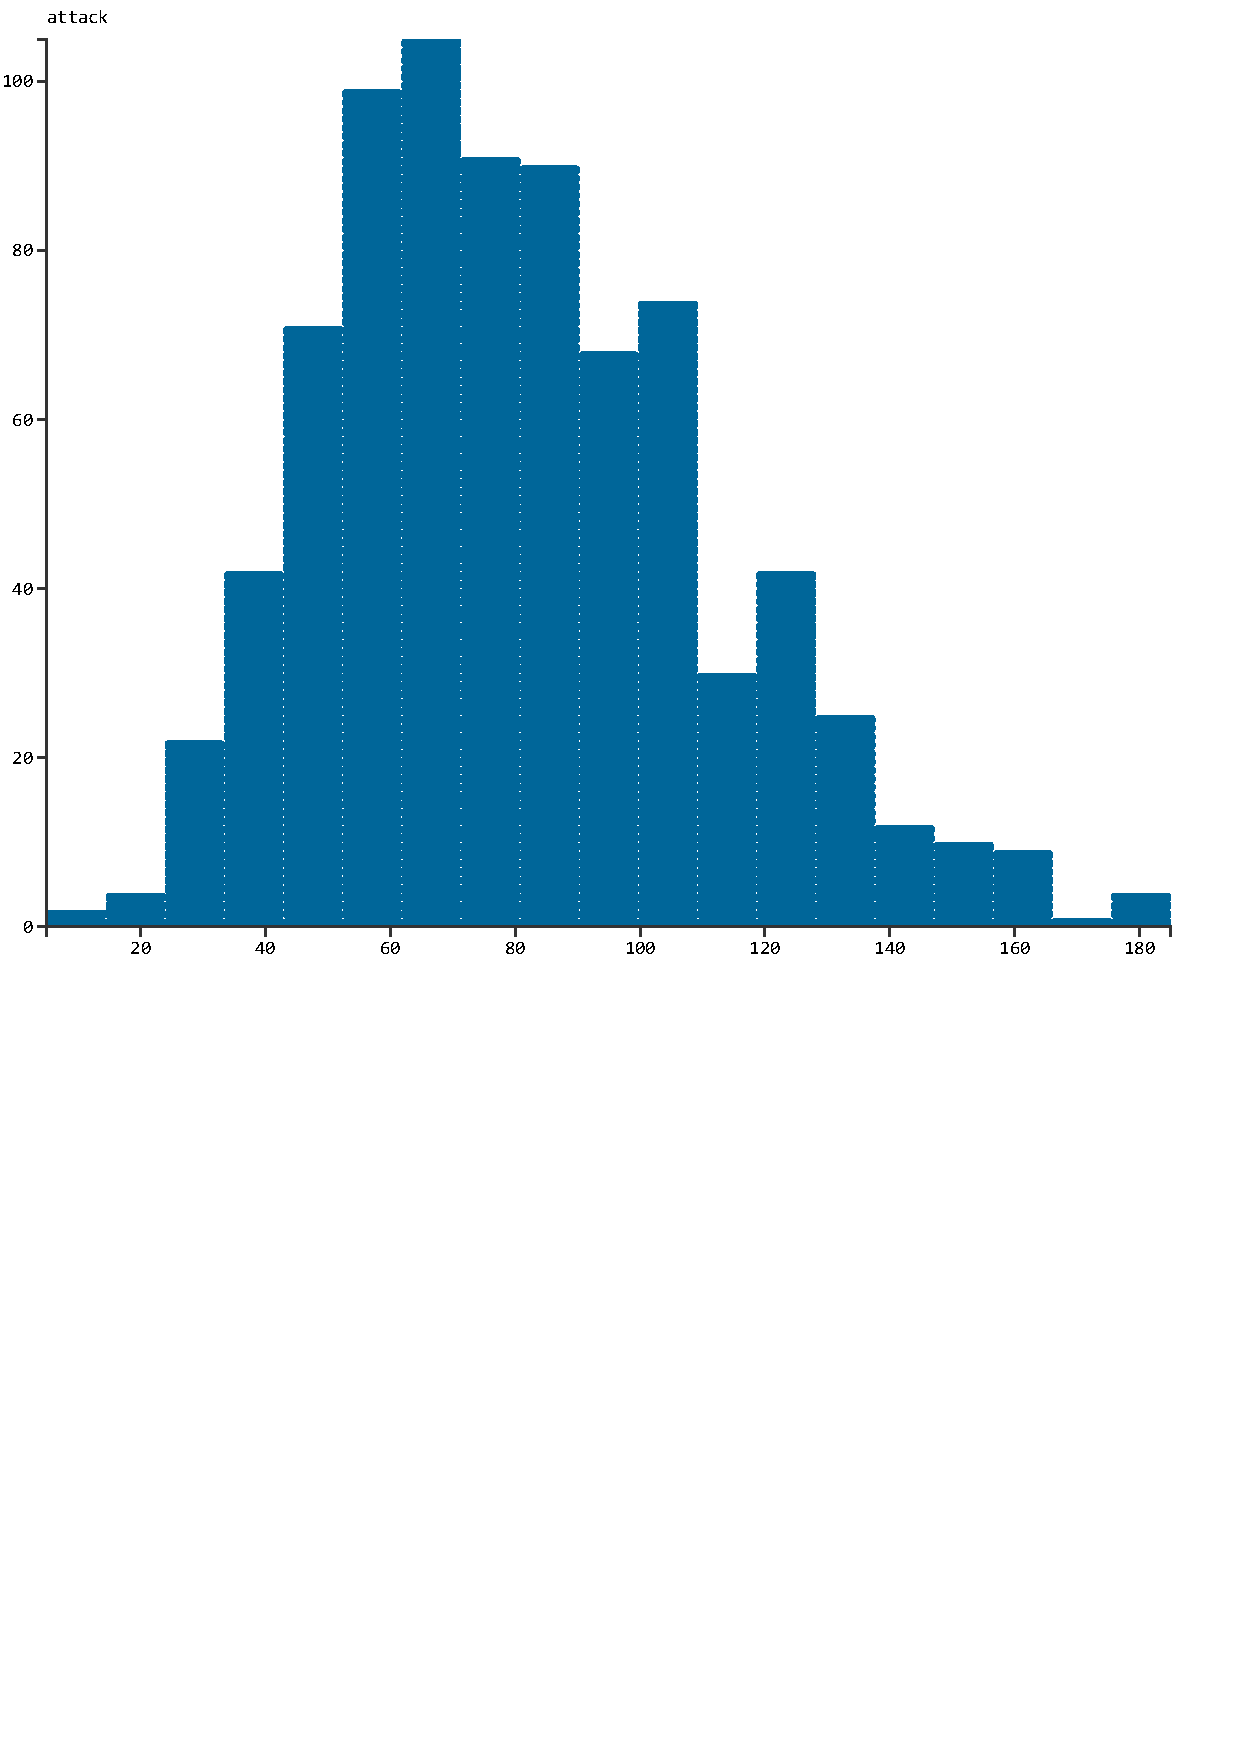
\includegraphics[width=40pc,size=1,trim={1cm 140mm, 1.5cm 50mm},clip]{figures/histograma.pdf}
	\end{center}
	\legend{Fonte: O autor}
\end{figure}
    
    \item  \textbf{Matriz de \textit{Scatter Plot}}:
    É uma técnica 2D onde reúne uma grade de gráficos de dispersão com valores que podem ser codificados para eixo X, eixo Y, cor e forma, sendo demonstrado sua implementação na ferramenta na \autoref{fig_matriz}.
    
    \begin{figure}
	\caption{\label{fig_matriz} exemplo da matriz de dispersão desenvolvida na ferramenta}
	\begin{center}
	    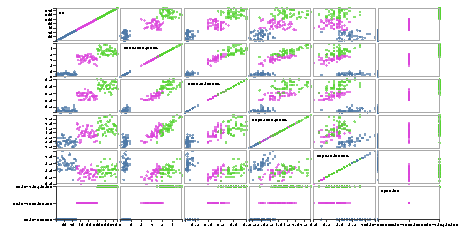
\includegraphics[width=40pc,height=30pc]{figures/scatterplot.pdf}
	\end{center}
	\legend{Fonte: O autor}
\end{figure}
    
    \item  \textbf{\textit{Parallel Bundling}}: É uma técnica de visualização baseada na técnica de coordenadas paralelas elaborada por \cite{divino2017visual} com as características de eixos e linhas semelhantes às coordenadas paralelas e com um agrupamento de arestas \cite{}, agrupando informações em um eixo onde pode conter características das informações do agrupamento dependendo da curva disposta para cada agrupamento   ilustrado na \autoref{fig_paralel_bundling}.
   
\begin{figure}
	\caption{\label{fig_paralel_bundling}Gráfico \textit{Parallel Bundling} gerado pela ferramenta desenvolvida }
	\begin{center}
	    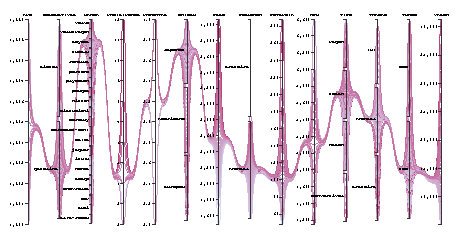
\includegraphics[width=40pc,height=25pc,size=1]{figures/parallel_bundle.pdf}
	\end{center}
	\legend{Fonte: O autor}
\end{figure}
    
    \item  \textbf{\textit{Sunburst}}:
    A técnica \textit{Sunburst} é uma visualização de dados em formato radial hierárquica, descrito por \cite{Stasko}  como uma árvore radial, ilustrada na \autoref{fig_sunb}, onde cada anel simboliza um nível de hierarquia tendo como centro o nó raiz, e os demais itens dos anéis podem ser divididos conforme os valores daquele nível, nas extremidades podemos ver nos respectivos nós folhas os dados de cada item como um fatia.
    
\begin{figure}
	\caption{\label{fig_sunb} Gráfico \textit{Sunburst} gerado na aplicação}
	\begin{center}
	    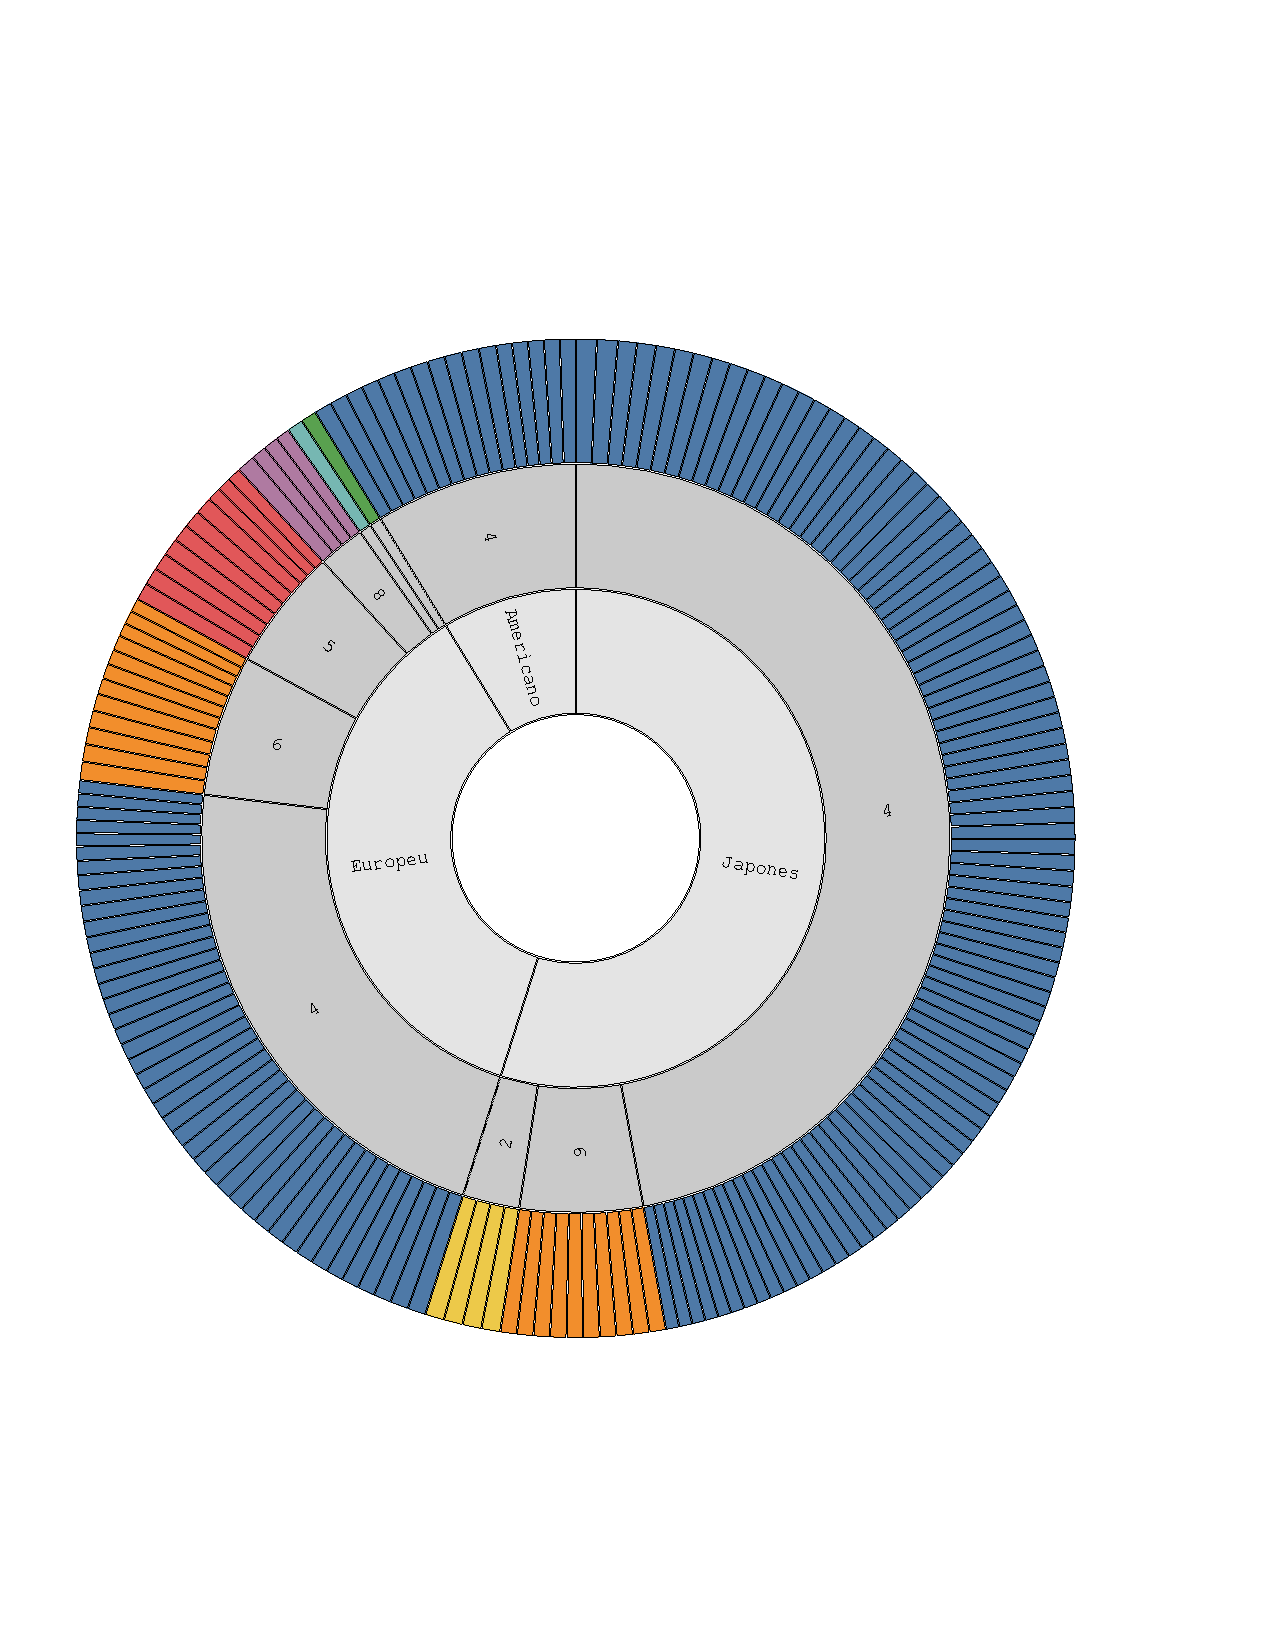
\includegraphics[width=40pc,size=1,trim={1cm 50mm, 1.5cm 50mm},clip]{figures/sunb.svg.pdf}
	\end{center}
	\legend{Fonte: O autor}
\end{figure}

    
    \item  \textbf{\textit{Treemap}}: A técnica  \textit{Treemap} foi desenvolvida por \cite{johnson1999tree} e tem como objetivo representar dados hierárquicos com uma proposta de preenchimento de espaços com itens retangulares. Nessa variação da técnica \textit{treemap} selecionada foi o \textit{treemap squarefid} a qual os item tentam manter uma estrutura retangular, onde as visualizações se adaptam ao espaço disponível e ocupam completamente o espaço. O \textit{treemap} pode conter organizações de hierarquias, serem atribuídas as cores, rótulos nos registros retangulares folhas ilustrado na \autoref{treemap}. 
      \begin{figure}
	\caption{\label{treemap}Gráfico treemap gerado pela ferramenta}
	\begin{center}
	    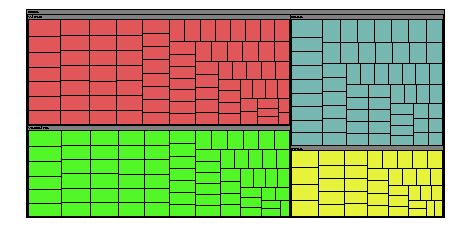
\includegraphics[width=40pc,height=30pc,size=1]{figures/treemap.pdf}
	\end{center}
	\legend{Fonte: O autor}
\end{figure}  
    
\end{itemize}


% \begin{figure}
% 	\caption{\label{tela_principal} Tela principal da ferramenta}
% 	\begin{center}
% 	    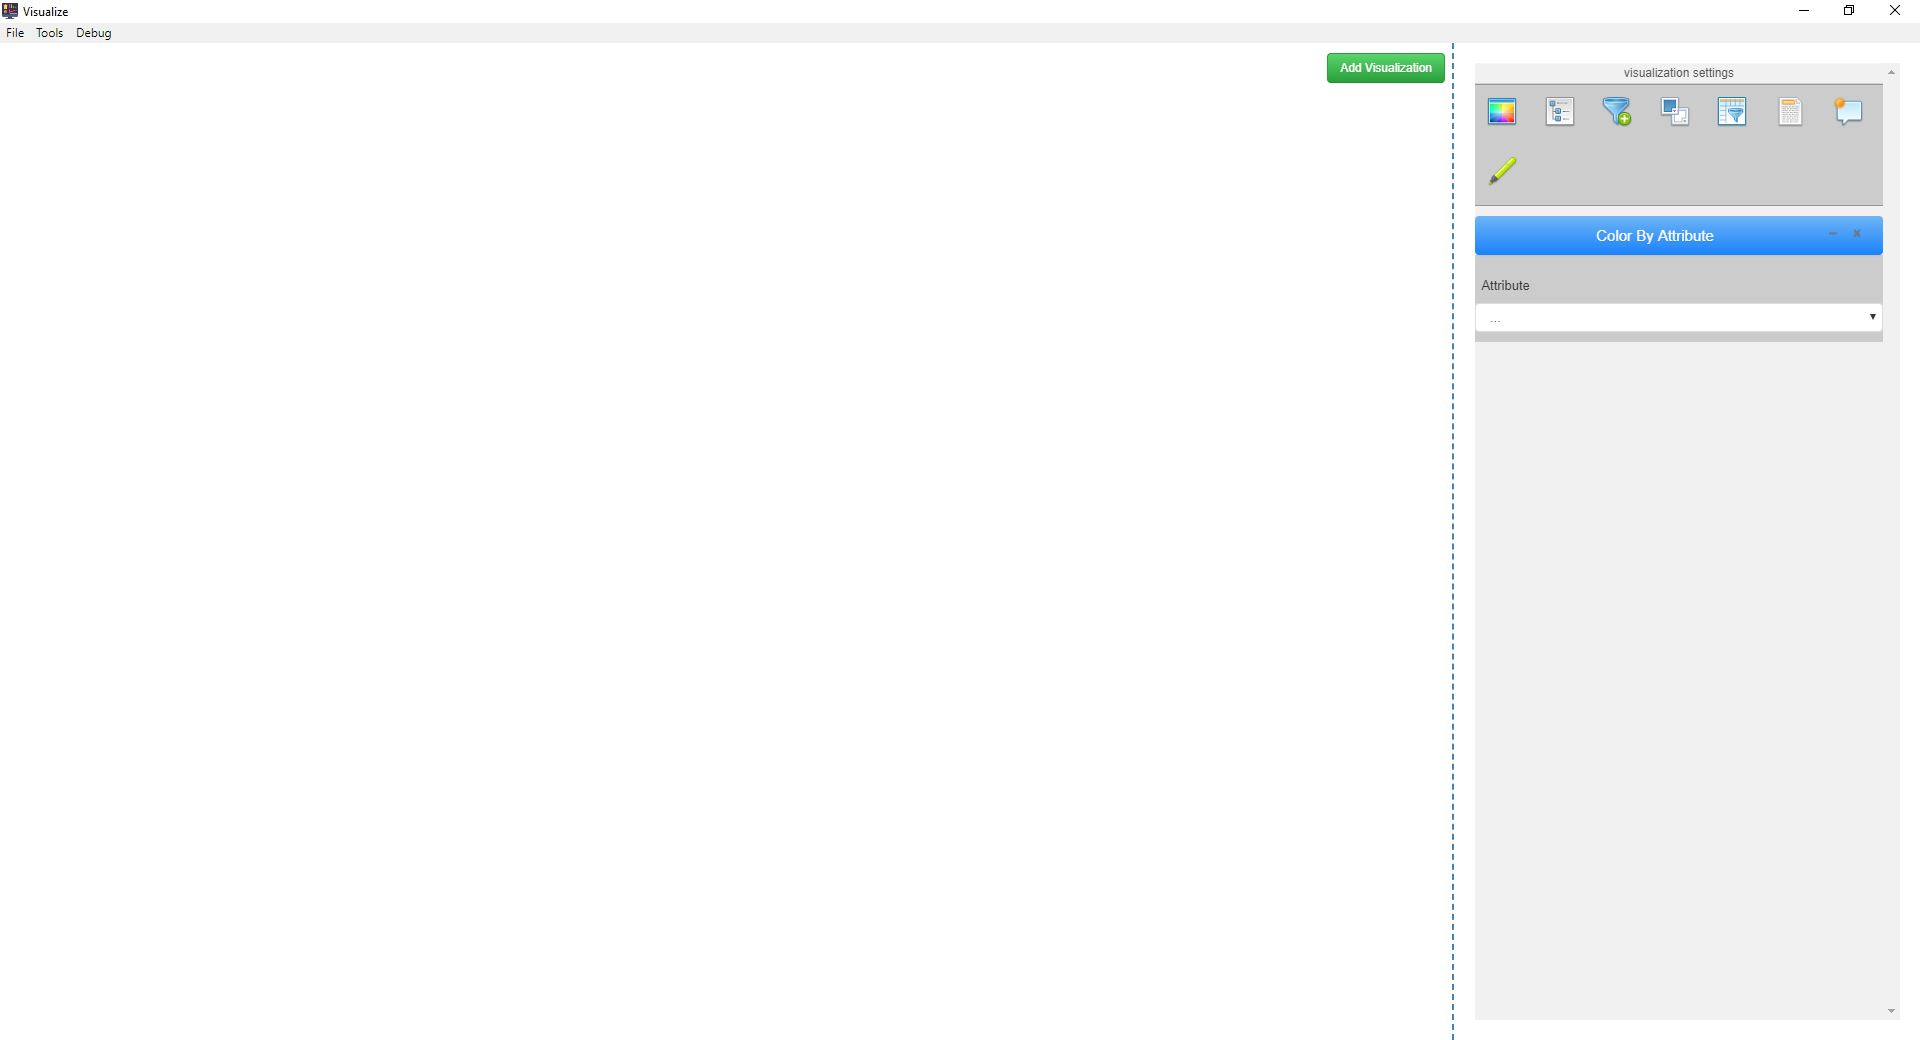
\includegraphics[width=50pc,size ,angle=90] {figures/ferramenta_tela_inicial.JPG}
% 	\end{center}
% 	\legend{Fonte: O autor}
% \end{figure}

\section{Funcionalidades}

O ambiente de criação das visualizações da ferramenta é um layout de partições redimensionáveis, demonstrado na \autoref{layout_divisors}, onde ficarão as visualizações, sendo possível configurar livremente o tamanho das visualizações, quais serão redimensionadas de acordo com o tamanho disponível, além disso, é possível utilizar as visualizações em ambientes de múltiplas telas e \textit{large display}, desse modo é  possível coordenar até 8 visualizações diferentes simultaneamente como ilustrado na \autoref{visualizations}.

\begin{figure}
	\caption{\label{visualizations}  Telas da aplicação com todas as visualizações disponíveis
}
	\begin{center}
	    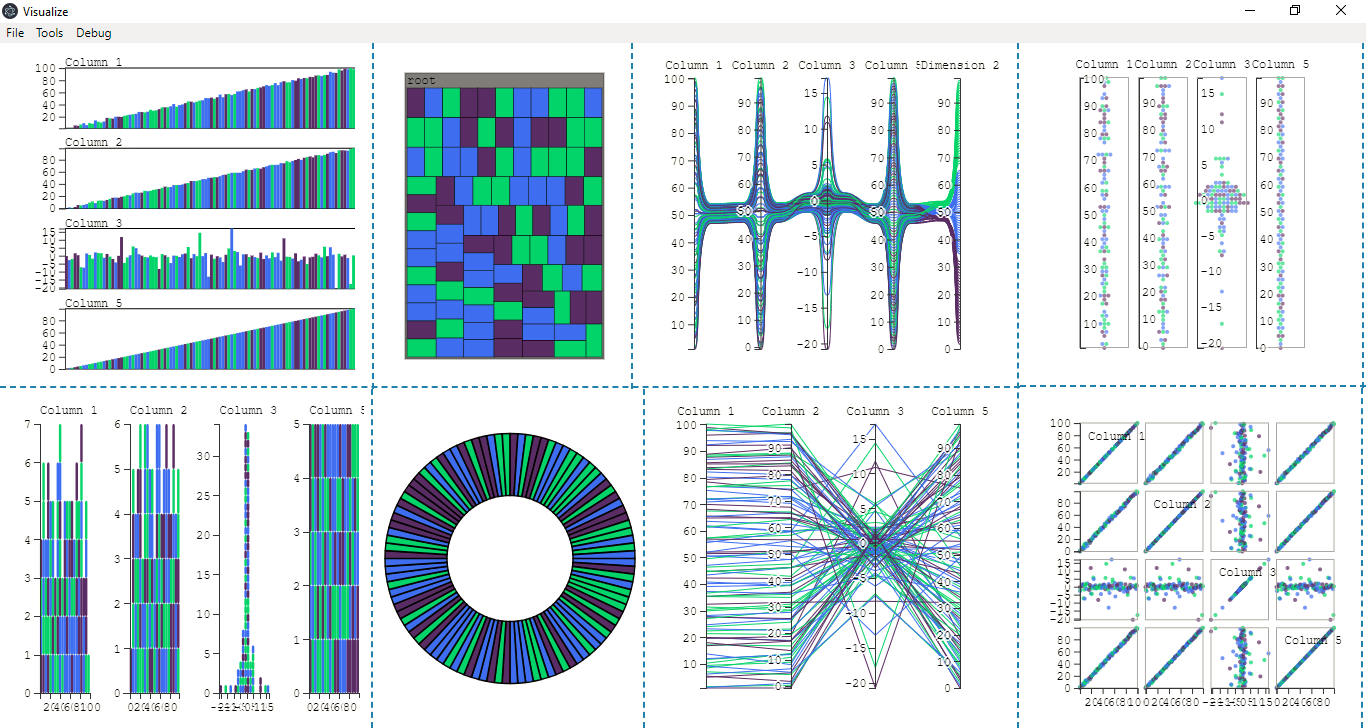
\includegraphics[width=42pc,size=1]{figures/Capturar1.PNG}
	\end{center}
	\legend{Fonte: O autor}
\end{figure}


\begin{figure}
	\caption{\label{layout_resize}  Telas de layout dinâmicos, as áreas destacadas representam: (1)- pontos representação redimensionar a tela, (2)- botão de criação das visualizações,(3) – criação de uma nova partição para visualizações.
}
	\begin{center}
	    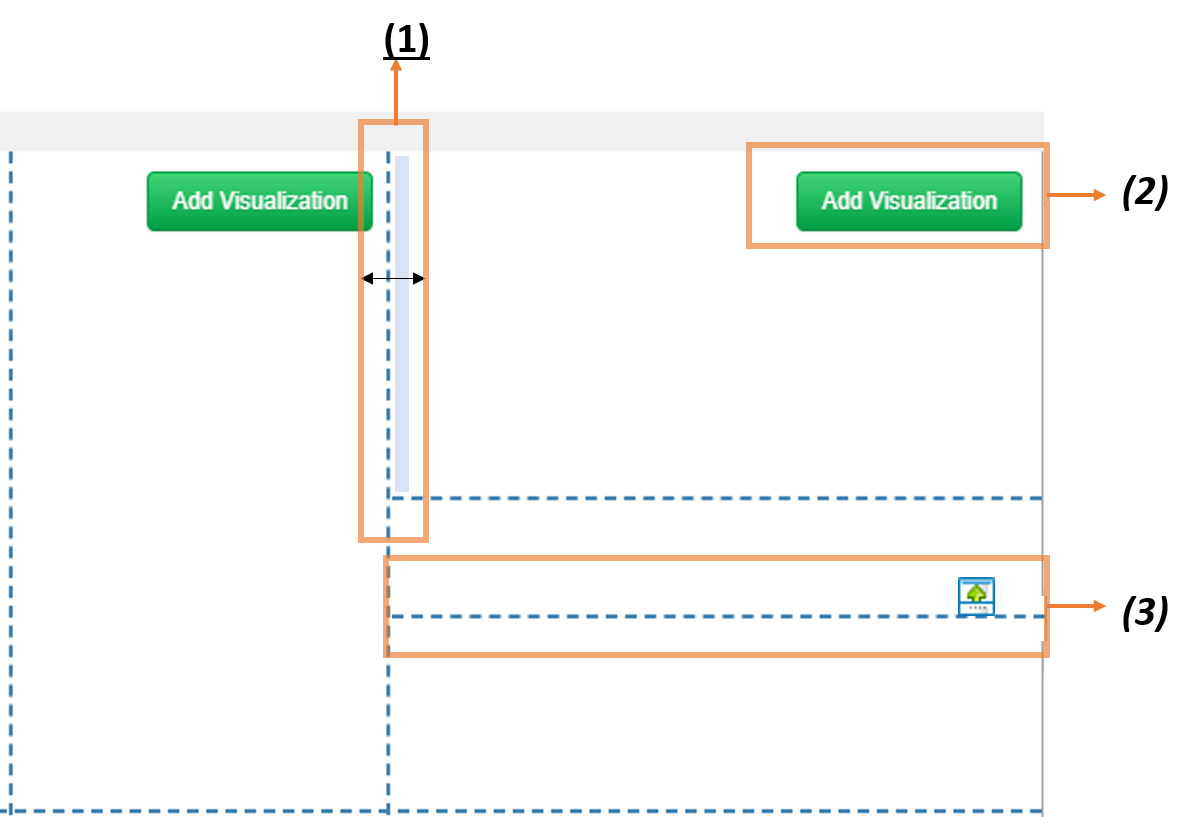
\includegraphics[width=30pc,scale=1]{figures/layouts.png}
	\end{center}
	\legend{Fonte: O autor}
\end{figure}

\section{Interações}
Segundo \cite{ward2010interactive} interações, no contexto de visualização de dados, são mecanismos disponíveis para modificar o que é visível pelo usuário. Existem diversas técnicas de interação como seleção, filtro, navegação, zoom, reconfigurar os dados e hierarquias, conectar dados em diferentes visualizações e objetos, e destaque. 

A ferramenta oferece interações e configurações, assim os usuários, seguindo os princípios de exploração visual:  \textit{“overview, first zoom and filter, then details-on-demand”} e seguindo os princípios principais de uma ferramenta de \textit{INFOVIS} definidos por \cite{Shneiderman1996}, a aplicação proporciona uma fácil manipulação e configuração das visualizações, com alta flexibilidade, permitindo filtros e seleções, sendo possível criar seleções, filtros, seleção de cor por atributo, hierarquias nas diversas visualizações. Sendo possível definir por meio das configurações de interfaces pelo usuário as interações e suas funcionalidades por meio dos ícones exemplificados na \autoref{img_icones}, no qual explica cada ícone de interação e suas respectivas funcionalidades.


\begin{figure}
	\caption{\label{img_icones}  Explicação do significado dos ícones de interação para as visualizações disponíveis.
}
	\begin{center}
	    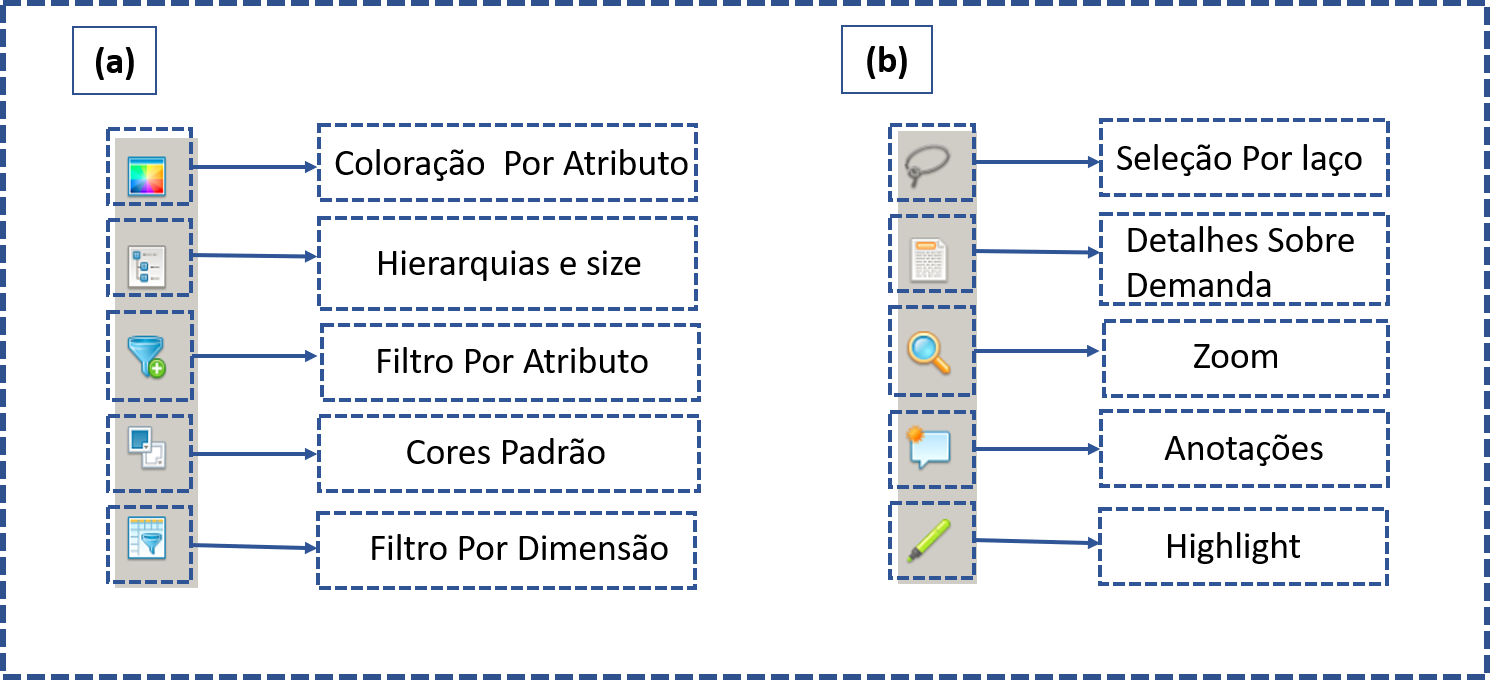
\includegraphics[width=20pc,scale=1]{figures/img_icones.png}
	\end{center}
	\legend{Fonte: O autor}
\end{figure}

     

\begin{itemize}
\item \textbf{Coloração por atributo}:
Nessa funcionalidade é possível selecionar atributos categóricos e contínuos, caso os atributos sejam categóricos a ferramenta permite a personalização de cor para cada atributo, caso sejam contínuos é possível escolher as cores do intervalo entre o valor mínimo e máximo. Bem como, cada visualização também vai seguir o padrão de cores selecionado para cada atributo.


A \autoref{fig_color_visualization} ilustra os menus de seleção de cor por atributo, onde no ponto "(a)" podemos ver uma seleção por atributos categóricos, na parte "(b)" é demonstrado o menus para atributos contínuos, e "(c)" o menu seletor de cores quando é selecionado um atributo. Do mesmo modo, ainda na \autoref{fig_color_visualization} no item "(d)" podemos ver duas visualizações utilizando o mesmo padrão de cores em um determinado atributo.

\begin{figure}
	\caption{\label{fig_color_visualization}  Exemplo de visualizações com coloração por um atributo contínuo e menu de interações para seleção de cores para atributos categóricos e contínuos.
}
	\begin{center}
	    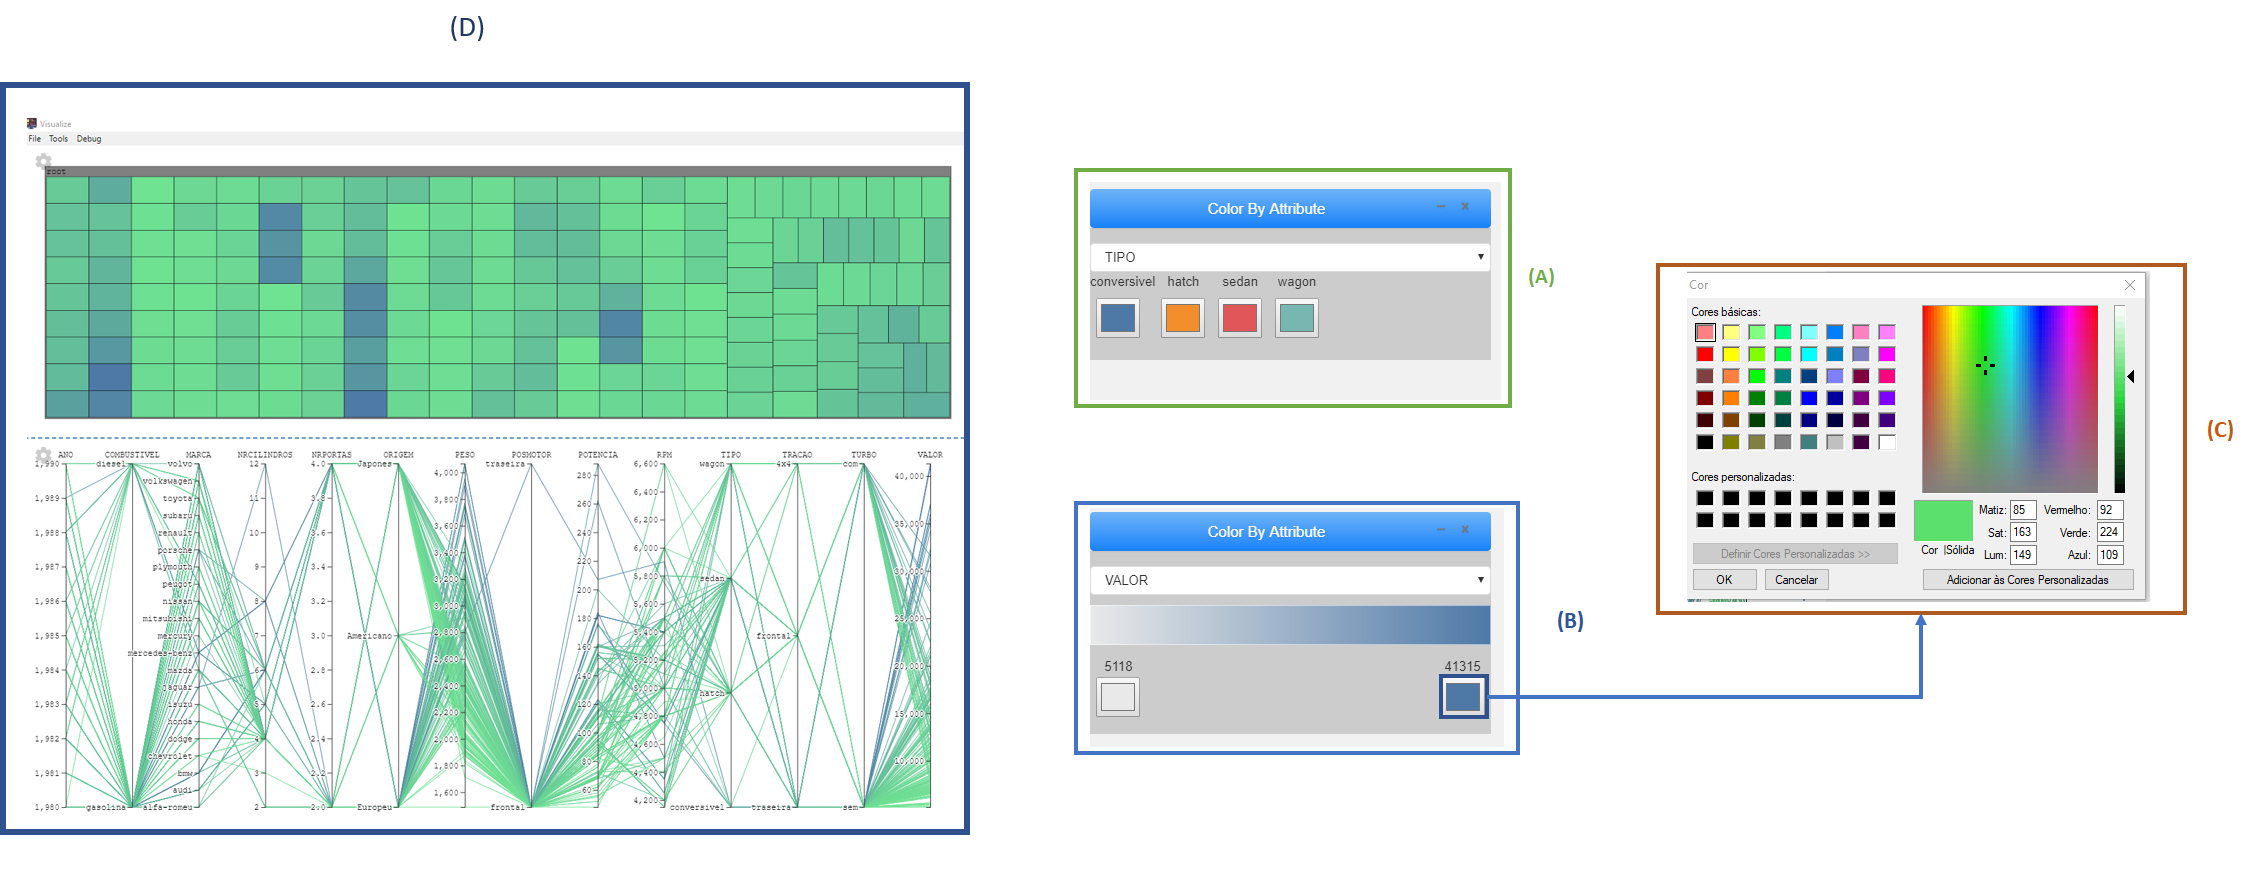
\includegraphics[width=40pc,height=25pc,scale=1]{figures/duas visualizações_2.png}
	\end{center}
	\legend{Fonte: O autor}
\end{figure}

\item \textbf{Filtros e Seleção}:
Na ferramenta existem dois tipos de filtros e seleções por atributo e por dimensão. Seleção e filtro por meio dos atributos tanto categóricos como contínuos. Caso seja escolhido um atributo categórico é disponibilizado um botão de seleção com as opções de cada atributo, caso o atributo seja contínuo é disponibilizado um \textit{slider} com o range entre o valor máximo e o mínimo como o exemplo da figura \autoref{fig_filtro_visualization}.

\begin{figure}
	\caption{\label{fig_filtro_visualization}  Exemplos do menu de filtro, (A) filtro menu de filtro contínuos e com um exemplo de visualização, (B) filtro menu categórico e visualização, (C) legenda menu de legenda de cores.
}
	\begin{center}
	    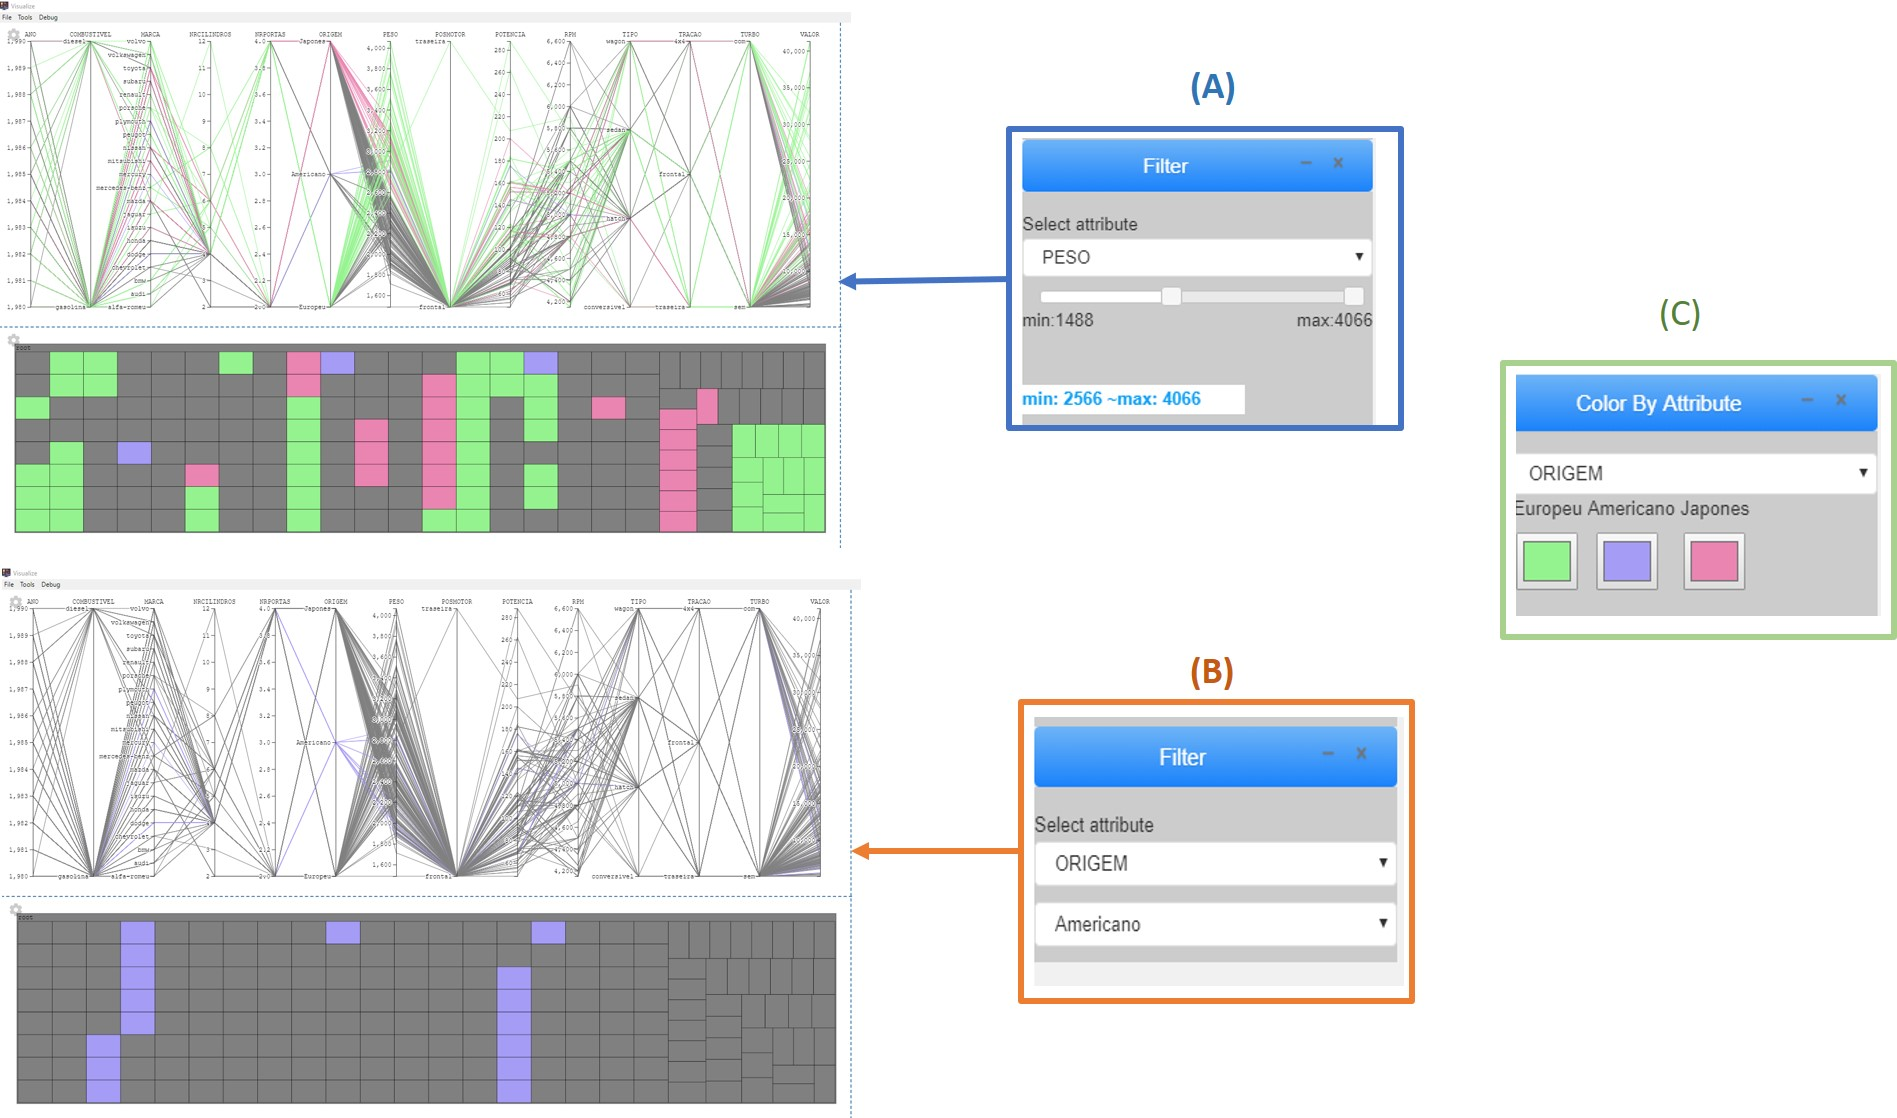
\includegraphics[width=40pc,scale=1]{figures/filtro.jpg}
	\end{center}
	\legend{Fonte: O autor}
\end{figure}

O filtro por dimensão dos dados pode ser utilizado em visualizações como \textit{scatterplot}, \textit{barchart}, \textit{histograma}, para dados multivariados foi implementado um filtro em uma dimensão de dados; no caso reduzindo um eixo ou parte da visualização correspondente a respectiva coluna da base de dados, reduzindo a visualização e dando maior ênfase nas partes de interesse como ilustrado na \autoref{fig_filtro_dimension_visualization}.

\begin{figure}
	\caption{\label{fig_filtro_dimension_visualization}  Exemplos do menu de filtro, (A) menu de filtro por dimensões e fluxo com filtro realizado nas visualização deixando apenas 4 dimensões.
}
	\begin{center}
	    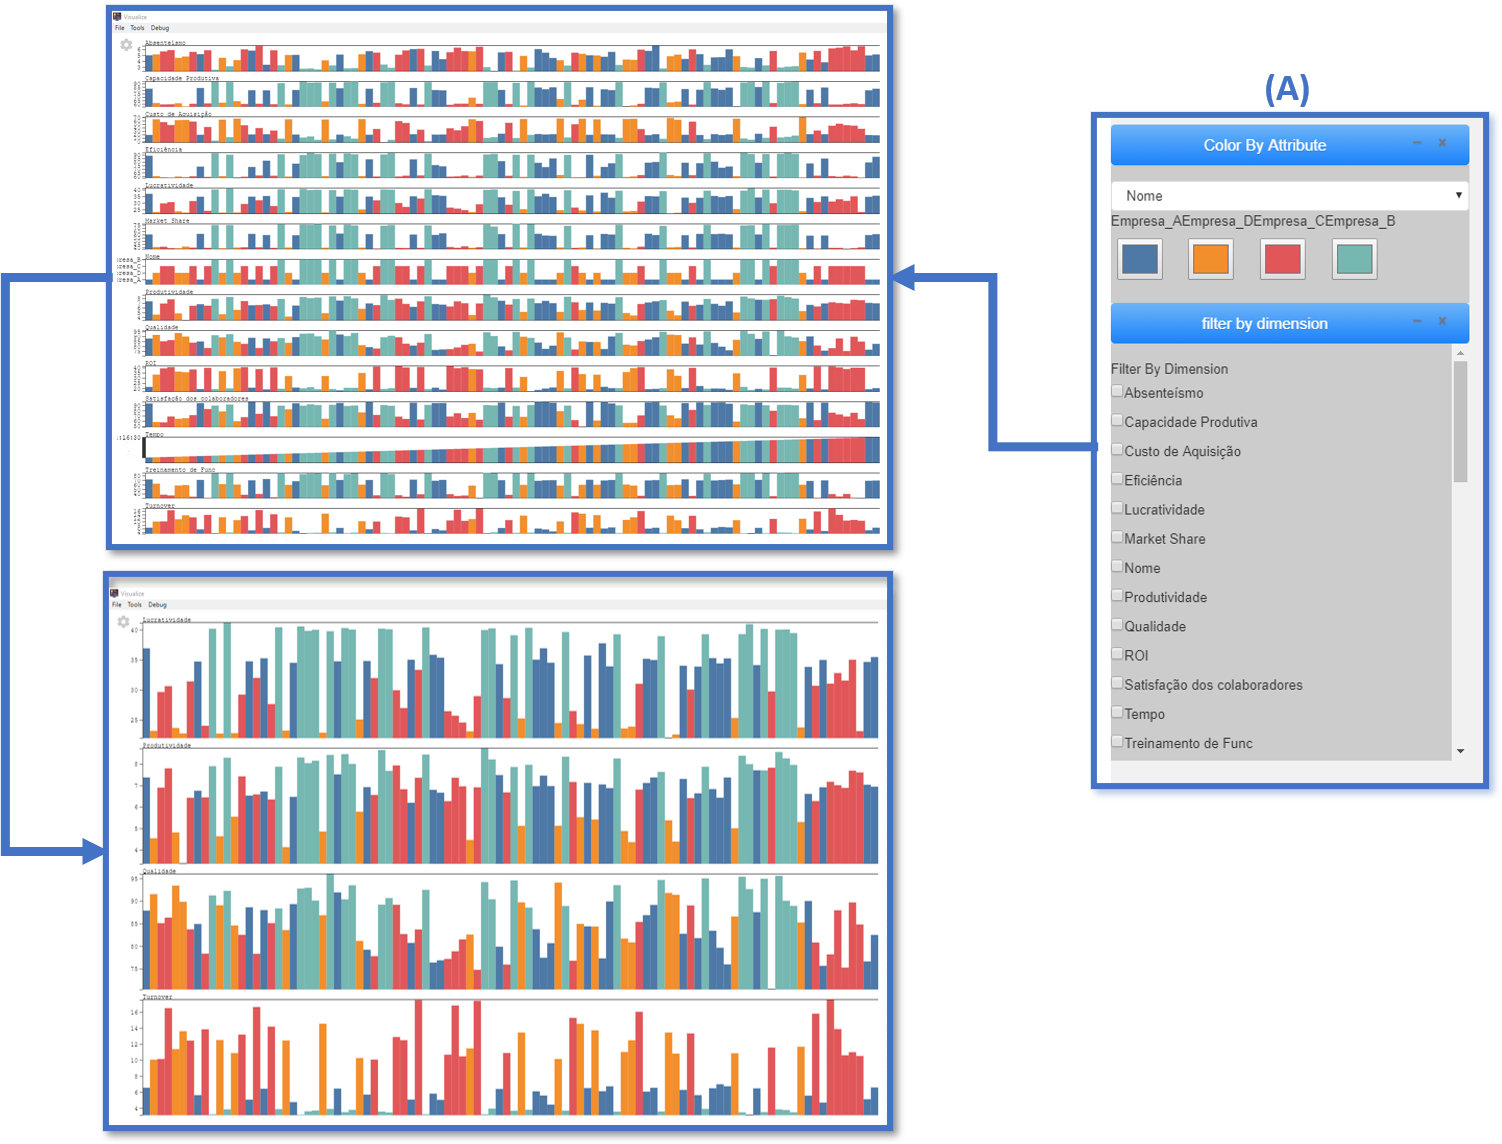
\includegraphics[width=40pc,scale=1]{figures/filtro_dimensao.png}
	\end{center}
	\legend{Fonte: O autor}
\end{figure}


\item \textbf{Criação de Hierarquias}:
O Controle de hierarquias pode ser feito em visualizações hierárquicas como \textit{treemap}, \textit{cicle packing}, e \textit{sunburst}, a ferramenta permite adicionar, remover estruturas hierárquicas nos dados, e decidir a ordem das hierarquias e também decidir qual atributo definirá o tamanho de cada item como pode ser visualizado na figura \autoref{vis_hierarquies}. 


\begin{figure}
	\caption{\label{vis_hierarquies}  Exemplo de visualizações hierárquicas na ferramenta. (A) representa menu de hierarquias onde podem ser selecionadas conforme os dados e definida a ordem, e o \textit{size} onde se define o tamanho dos itens nas visualizações. (B) representa o atributo selecionado para as core na visualização.
}
	\begin{center}
	    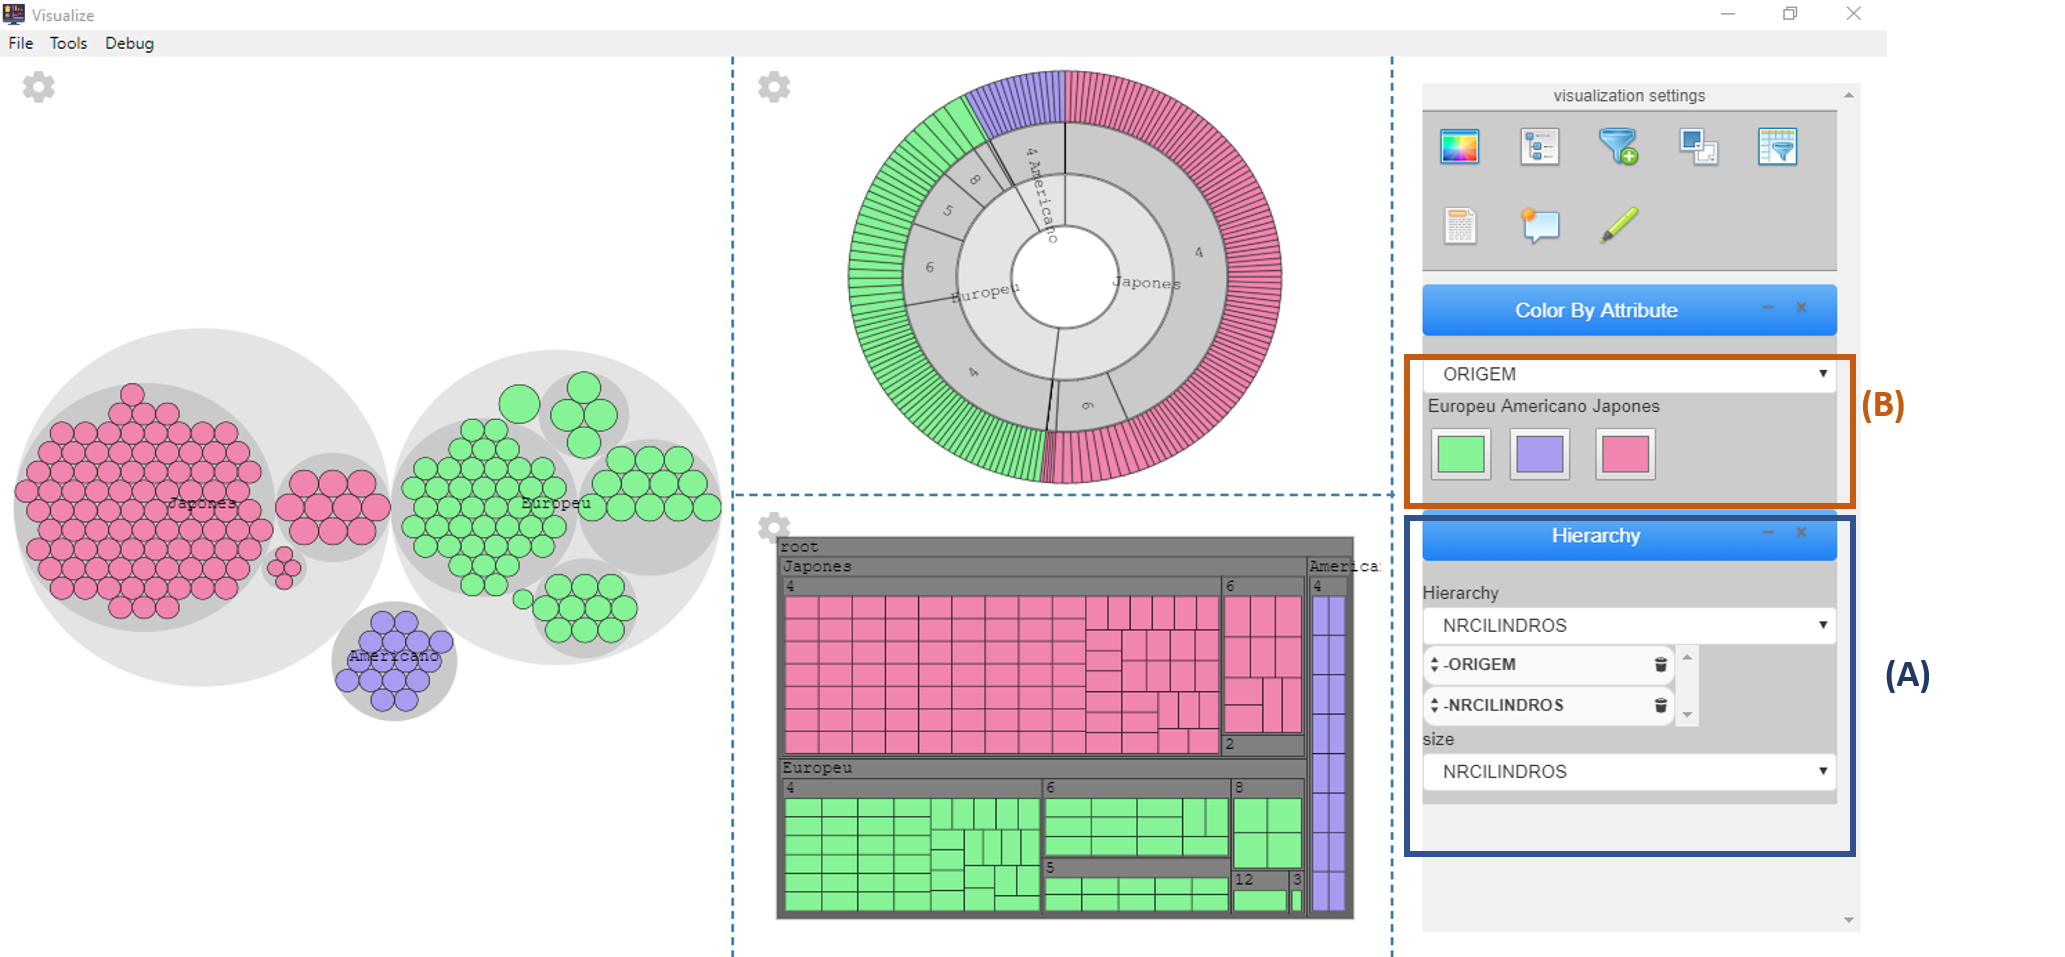
\includegraphics[width=40pc,scale=1]{figures/hierarquias.png}
	\end{center}
	\legend{Fonte: O autor}
\end{figure}

\item \textbf{Detalhes sobre Demanda}:
Interação de detalhes sobre demanda configurável quando mouse é passado sobre o item.

\item \textbf{Destaque}: Por meio de seleção do mouse e clique ou passagem do mouse de maneira coordenadas nas visualizações, por exemplo em caso de várias visualizações no \textit{dashboard}, o mesmo item será destacado nos diferentes a gráficos. A \autoref{vis_destaque} ilustra essa situação.
\begin{figure}
	\caption{\label{vis_destaque}  Exemplo de duas visualizações com destaque no item de maneira coordenada.
}
	\begin{center}
	    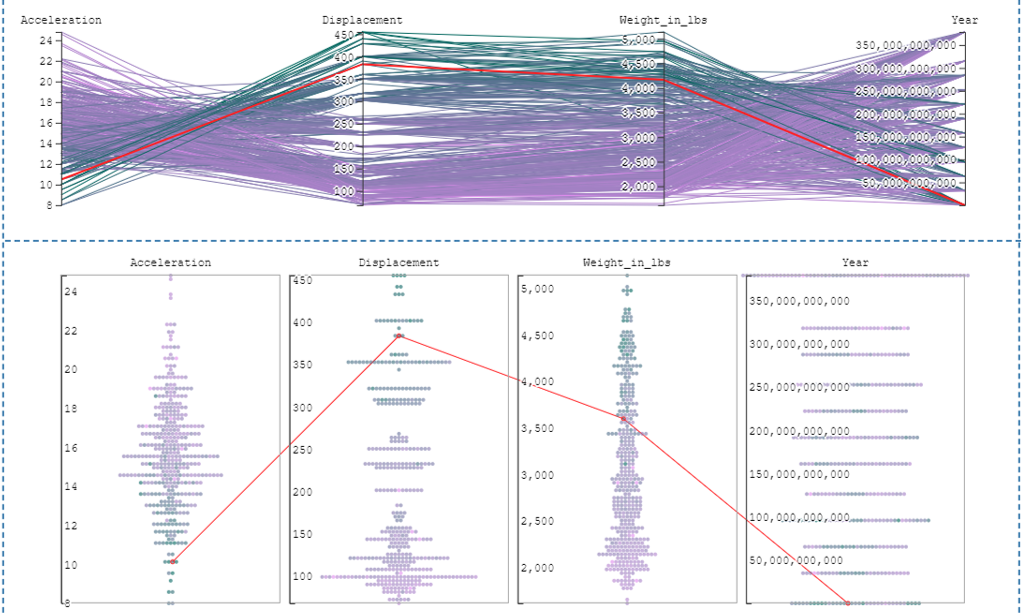
\includegraphics[width=35pc,scale=1]{figures/cordinate_highliht.png}
	\end{center}
	\legend{Fonte: O autor}
\end{figure}

\item \textbf{Anotações}: Interação de anotações sobre os itens da base de dados, podendo ser personalizadas, exemplo \autoref{vis_anotacao}.

\begin{figure}
	\caption{\label{vis_anotacao}  Exemplo de anotações no beeswarmplot.
}
	\begin{center}
	    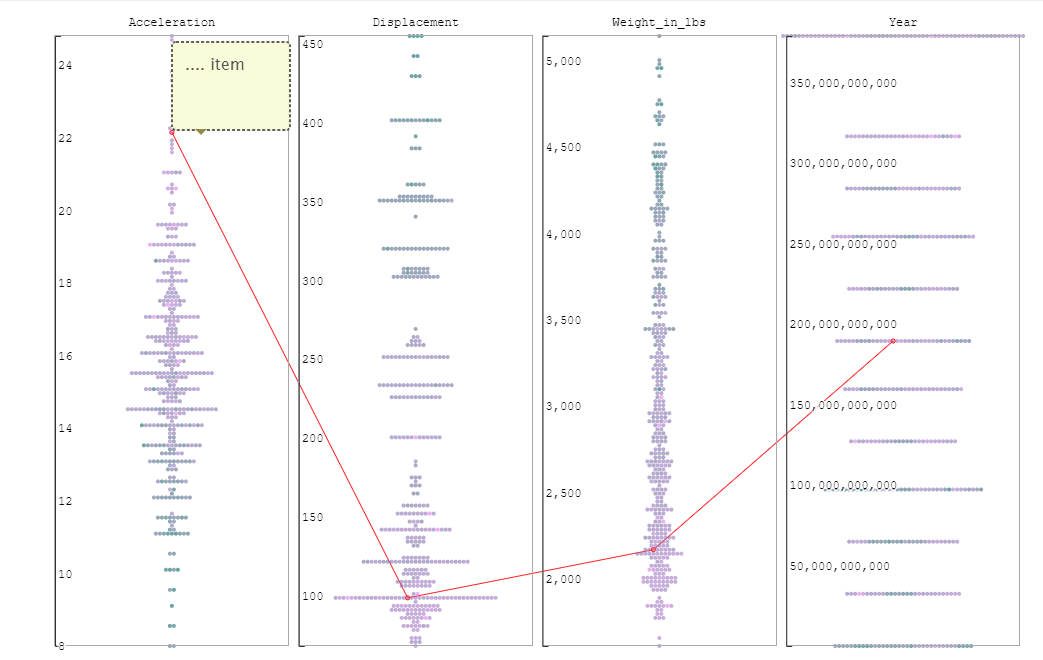
\includegraphics[width=35pc,scale=1]{figures/anottation.png}
	\end{center}
	\legend{Fonte: O autor}
\end{figure}


\end{itemize}

\chapter{Base de dados de Validação}
\label{ch:base}

A geração de uma base de dados sintética foi realizada na ferramenta Blocks \cite{blocks}, simulando um cenário de 4 empresas fictícias em situação de competição. Seguindo os KPI's selecionados para criação da base sintética.


\section{Descrição da Base}

\begin{center}
\caption{Indicadores Baseados nos Quadrantes do BSC}\\
\label{tabela_indicadores}
\begin{tabular}{l|l|l|l}
\hline
Processos Internos & Financeiro & Clientes & Aprendizado e Crescimento\\
\hline
Produtividade & Lucratividade & Satisfação do Cliente & Turnover\\
Capacidade Produtiva & Faturamento & Aquisição de Clientes & Treinamento de Funcionários\\
Eficiência & Ticket Médio & Retenção de Clientes & Satisfação dos Colaboradores\\
Qualidade & ROI & Market Share & Absenteísmo\\
\hline

\end{tabular}
\end{center}

Dentro dos indicadores dos Processos Internos, temos a Produtividade(PRO). Este indicador representa a produtividade da equipe medida a partir das horas trabalhadas e o tamanho da atividade ou do produto desenvolvido. Como o próprio nome informa, o objetivo estratégico associado a este indicador é o aumento da produtividade da equipe. As metas e limites utilizados como métrica de medição foram:
\begin{itemize}
\item  \textbf{\textit{OK}}: acima de 8Pts/H;
\item  \textbf{\textit{Alerta}}: entre 6 e 8Pts/H;
\item  \textbf{\textit{Crítico}}: abaixo de 6Pts/H.
\end{itemize}

Neste caso, utilizou-se Pontos (Pts) para representar o tamanho de atividades ou produtos, mas isso deve ser adaptado para realidade de cada organização. Pensou-se em um contexto no qual a produtividade máxima seria representada por 10pts produzidos em uma hora. A fórmula que melhor representa a medida é: PRO = Pts/H. Onde (Pts) são os pontos da tarefa e (H) as horas utilizadas para executar a tarefa, utilizando decimal como unidade de medida.

A Capacidade Produtiva(CAP) é o próximo indicador dentro dos Processos Internos. Onde representa a capacidade máxima que a organização pode produzir em um período com os recursos que tiver à sua disposição. O objetivo estratégico associado é saber se a empresa consegue atender adequadamente à demanda solicitada por seus clientes. Ou ainda, se precisará realizar algum ajuste. Seja no quadro de funcionários ou processos, caso a capacidade esteja muito acima ou abaixo em relação à demanda. As metas e limites utilizados como métrica serão:
\begin{itemize}
\item  \textbf{\textit{OK}}: acima de 90\%;
\item  \textbf{\textit{Alerta}}: entre 80\% e 90\%;
\item  \textbf{\textit{Crítico}}: abaixo de 80\%.
\end{itemize}

A fórmula para representar essas metas e limites pode ser melhor descrita como CAP = (PDA/PDT), onde (PDA) é a produção atual e (PDT) a produção total, utilizando percentual como unidade de medida.

O próximo indicador apresentado dentro dos Processos Internos é a Eficiência(EFC). Representa a capacidade de produzir mais consumindo menos recursos. Onde o seu objetivo estratégico associado é conseguir o melhor rendimento com o mínimo de erros e/ou dispêndios. As metas e limites indicados são:
\begin{itemize}
\item  \textbf{\textit{OK}}: acima de 85\%;
\item  \textbf{\textit{Alerta}}: entre 70\% e 85\%;
\item  \textbf{\textit{Crítico}}: abaixo de 70\%.
\end{itemize}

A fórmula apresentada é EFC = PDE/PDP, onde (PDE) é a produção efetiva e (PDP) é a produção planejada, utilizando também o percentual como unidade de medida.

Por fim, temos a Qualidade(QUA) como o último indicador dos Processos Internos. Onde apresenta um conceito subjetivo, porém de maneira geral é o grau de excelência do que é entregue como produto ou serviço, estando conforme e consistente com as expectativas dos clientes e em conformidade com normas e requisitos funcionais, adequado à finalidade para a qual foi projetado. Tendo como foco do objetivo estratégico aumentar a qualidade dos produtos/serviços entregues. As metas e limites serão representados por: 
\begin{itemize}
\item  \textbf{\textit{OK}}: maior ou igual a 95\% dos defeitos que foram identificados antes do projeto ser entregue ao cliente;
\item  \textbf{\textit{Alerta}}: entre 80\% e 94,9\% dos defeitos que foram identificados antes do projeto ser entregue ao cliente;
\item  \textbf{\textit{Crítico}}: abaixo de 79,9\% dos defeitos que foram identificados antes do projeto ser entregue ao cliente.
\end{itemize}

A fórmula que melhor representa essas medidas é QUA = TDI/(TDI+TDE)*100. Onde (TDI) é o total de defeitos internos e (TDE) o total de defeitos externos. Utilizando percentual como unidade de medida.

O primeiro indicador apresentado para o quadrante Financeiro é a Lucratividade(LUC). Este indicador mede a capacidade operacional do empreendimento em gerar lucros a partir de um projeto desenvolvido. Tendo como objetivo estratégico aumentar o lucro da organização. As metas e limites definidos como métricas são representadas por:
\begin{itemize}
\item  \textbf{\textit{OK}}: acima de 25\%;
\item  \textbf{\textit{Alerta}}: entre 10\% e 25\%;
\item  \textbf{\textit{Crítico}}: abaixo de 25\%.
\end{itemize}

A formula que descreve essas metas e limites é LUC = (LUL/REC) x 100. Onde (LUL) é o lucro líquido  e (REC) a receita total, utilizando percentual como unidade de medida.

O segundo indicador do quadrante Financeiro é o Faturamento(FAT). Onde representa a soma de todas as vendas realizadas ou serviços prestados em um determinado período. Onde seu objetivo estratégico é determinar a performance de vendas, entendendo-se se o preço cobrado está dentro da expectativa dos consumidores. Apresentando as metas e limites abaixo:
\begin{itemize}
\item  \textbf{\textit{OK}}: acima de 60\% do limite de faturamento do porte da empresa;
\item  \textbf{\textit{Alerta}}: entre 40\% e 60\% do limite de faturamento do porte da empresa;
\item  \textbf{\textit{Crítico}}: abaixo de 40\% do limite de faturamento do porte da empresa.
\end{itemize}

A fórmula apresentada para descrever essas métricas é FAT = (SVE/FPE) x 100. Onde (SVE) é a soma do valor de entrada e (FPE) o faturamento do porta da empresa. Sendo o percentual utilizado como unidade de medida.

O terceiro indicador do quadrante Financeiro é o Ticket Médio(TME). Indicando o valor gasto, em média, por cada cliente dentro do negócio. Tendo como objetivo estratégico melhorar a performance de vendas e adequar o valor do produto/serviço fornecido. As metas e limites são apresentados por:
\begin{itemize}
\item  \textbf{\textit{OK}}: acima de 300\% do custo da aquisição por cliente;
\item  \textbf{\textit{Alerta}}: entre 150\% e 300\% do custo da aquisição por cliente;
\item  \textbf{\textit{Crítico}}: abaixo de 150\% do custo da aquisição por cliente.
\end{itemize}

A fórmula utilizadas para representar essas metas e limite é TME = (FTP/NPP) x 100. Onde (FTP) é o faturamento total no período e (NPP) é o número de pedidos no período. Utilizando também o percentual como unidade de medida.

Finalizando temos com o Retorno sobre Investimento(ROI) como quarto indicador do quadrante Financeiro. Retorno sobre investimento (em inglês, return on investment ou ROI), também chamado de  taxa de retorno, taxa de lucro ou simplesmente retorno, é a relação entre a quantidade de dinheiro ganho (ou perdido) como resultado de um investimento e a quantidade de dinheiro investido. Seu objetivo estratégico é aumentar o retorno em relação ao investimento. As metas e limites são apresentados por:
\begin{itemize}
\item  \textbf{\textit{OK}}: acima de 20\%;
\item  \textbf{\textit{Alerta}}: entre 30\% e 40\%;
\item  \textbf{\textit{Crítico}}: abaixo de 40\%.
\end{itemize}

A fórmula que representa as métricas apresentadas acima é ROI = (REC - CUS) CUS x 100. Onde (REC) é a receita e (CUS) o custo. O percentual também é unidade de medida utilizada. 

O primeiro indicador do quadrante Clientes é a Satisfação do Cliente(SCL). Apresentando o sentimento de prazer ou de desapontamento resultante da comparação do desempenho esperado pelo produto (ou resultado) em relação às expectativas da pessoa. O objetivo estratégico associado a esse indicador foca em aumentar a satisfação dos clientes. As metas e limites podem ser medidos como:
\begin{itemize}
\item  \textbf{\textit{OK}}: acima de 90\%;
\item  \textbf{\textit{Alerta}}: entre 70\% e 90\%;
\item  \textbf{\textit{Crítico}}: abaixo de 70\%.
\end{itemize}

A fórmula que melhor descreve essas métricas é SCL = SPS/NPR. Onde (SPR) é o somatório do percentual de satisfação e (NPR) o número de pesquisas respondidas. Utilizando o percentual como unidade de medida.

O segundo indicador do quadrante Clientes é o Custo de Aquisição por Clientes(CAC). O Custo de Aquisição de Clientes (CAC) é um dos principais indicadores de vendas usado por empresas para medir o quanto custa conquistar um cliente. O CAC inclui desde custos de marketing até os salários e comissões dos vendedores que atuam ativamente na venda de uma solução, produto ou serviço. O objetivo estratégico é otimizar a relação custo benefício de aquisição e retorno de clientes. As metas e limites podem ser apresentados por:
\begin{itemize}
\item  \textbf{\textit{OK}}: abaixo de 33\% do valor do ticket médio;
\item  \textbf{\textit{Alerta}}: entre 33\% e 66\% do valor do ticket médio;
\item  \textbf{\textit{Crítico}}: acima de 66\% do valor do ticket médio.
\end{itemize}

Essas metas e limites são representadas pela fórmula CAC = (SOI/NCA) x 100. Onde (SOI) é a soma dos investimentos e (NCA) o número de clientes adquiridos. A unidade de medida utilizada também pelo percentual.

O terceiro indicador do quadrante Clientes é a Retenção de Clientes(RTC). Onde se caracteriza pelas ações relacionadas para reduzir o número de perdas de clientes. Tem como objetivo estratégico manter o máximo números de clientes ativos. As metas e limites são definidos como:
\begin{itemize}
\item  \textbf{\textit{OK}}: acima de 65\%;
\item  \textbf{\textit{Alerta}}: entre 40\% e 65\%;
\item  \textbf{\textit{Crítico}}: abaixo de 40\%.
\end{itemize}

A fórmula que melhor representa essas métricas é RTC = (CLA/TOC) x 100. Onde (CLA) são os clientes ativos e o (TOC) o total de clientes. Utilizando também o percentual como unidade de medida.

O quarto e último indicador do quadrante Clientes é o Market Share(MKS). Este indicador se refere à participação no mercado em relação a aspectos como volume de vendas, faturamento, quantidade de clientes, lucratividade, etc. Seu objetivo estratégico é intensificar a participação no mercado. Podemos definir as metas e limites como:
\begin{itemize}
\item  \textbf{\textit{OK}}: acima de 20\%;
\item  \textbf{\textit{Alerta}}: entre 8\% e 20\%;
\item  \textbf{\textit{Crítico}}: abaixo de 8\%.
\end{itemize}

A fórmula para representar as métricas declaradas é MKS = (REO/RTM) x 100. Onde (REO) é o resultado específico da organização e (RTM) o resultado total do mercado. Utilizando o percentual como unidade de medida.

O primeiro indicador do quadrante Aprendizado e Crescimento é o Turnover(TUR). Este indicador é responsável por medir a quantidade de colaboradores desligados/admitidos de uma empresa em relação ao número de colaboradores no quadro funcional. Seu objetivo estratégico associado é reter talentos a fim de manter o capital intelectual na organização. As metas e limites foram definidos por:
\begin{itemize}
\item  \textbf{\textit{OK}}: abaixo de 5\%;
\item  \textbf{\textit{Alerta}}: entre 5\% e 10\%;
\item  \textbf{\textit{Crítico}}: acima de 20\%.
\end{itemize}

Sua fórmula pode ser representada por TUR = (MAD/NFI) x 100. Onde (MAD) é a média de admissões e desligamentos e (NFP) o número de funcionários do início do período. Percentual também é sua unidade de medida.

O segundo indicador do quadrante Aprendizado e Crescimento é o Treinamento de Funcionários(TRF). O indicador visa medir a eficiência da educação corporativa. Seu objetivo estratégico é melhorar a capacitação dos colaboradores da organização. Suas metas e limites foram representados por:
\begin{itemize}
\item  \textbf{\textit{OK}}: acima de 70\%;
\item  \textbf{\textit{Alerta}}: entre 50\% e 70\%;
\item  \textbf{\textit{Crítico}}: abaixo de 50\%.
\end{itemize}
 
A fórmula que representa os valores das metas e limites é TRF = (TRR/TRP) x 100. Onde (TRR) são os treinamentos realizados e o (TRP) os treinamentos planejados. Utilizando o percentual como unidade de medida.

O terceiro indicador do quadrante Aprendizado e Crescimento é a Satisfação dos Colaboradores(SCO). Tal indicador refere-se ao nível de felicidade, satisfação e motivação dos colaboradores em seus trabalhos. Seu objetivo estratégico é aumentar a satisfação e motivação dos colaboradores em trabalhar na organização. Suas metas e limites são definidos por: 
\begin{itemize}
\item  \textbf{\textit{OK}}: acima de 90\%;
\item  \textbf{\textit{Alerta}}: entre 70\% e 90\%;
\item  \textbf{\textit{Crítico}}: abaixo de 70\%.
\end{itemize}

A fórmula que melhor representa essas métricas é SCO = SPS/NPR. Onde (SPR) é o somatório do percentual de satisfação e (NPR) o número de pesquisas respondidas. Utilizando o percentual como unidade de medida.

O quarto e último indicador do quadrante Aprendizado e Crescimento é o Absenteísmo(ABS). Absenteísmo no trabalho ou ausentismo é um padrão de falta dos funcionários por motivos que não doenças, desemprego ou licença. Seu objetivo estratégico é eliminar e/ou manter baixo o índice de absenteísmo na organização. As metas e limites definidos são:
\begin{itemize}
\item  \textbf{\textit{OK}}: até 5\%;
\item  \textbf{\textit{Alerta}}: entre 5\% e 10\%;
\item  \textbf{\textit{Crítico}}: acima de 10\%.
\end{itemize}

A fórmula que representa os valores obtidos para essas métricas é ABS = (NHP/THT) x 100. Onde (NHP) é o número de horas perdidas e o (THT) o número de horas totais que deveriam ser executadas. Utilizando também o percentual como unidade de medida.



\section{Construção da Base}
A construção de uma base de dados sintética foi realizada para validar e gerar visualizações na ferramenta, no contexto de empresas em concorrência. 
Os geradores de dados para criação da base sintética de dados selecionados nos blocks foram divididos em 4 tipos, Processos Internos, Financeiro, Clientes, Aprendizado e Crescimento.
O atributo “nome” foi selecionado do tipo “categorical” criando uma coluna para definir qual a empresa pertencente, no caso foram definidas como \textbf{“empresaA”}, \textbf{”empresaB”},  \textbf{“empresaC”}, \textbf{"empresaD"}.

Os demais atributos "numéricos" \ foram gerados seguindo mesmo padrão, foi selecionado o gerador \textit{“categorical Function”} onde permite selecionar um atributo categórico e para cada tipo de valor categórico contido nessa coluna gerar um numérico diferente variando entre \textit{“Gaussian Generator”} um gerador que cria valores em uma gaussiana entre um determinado intervalo e \textit{“Uniform Generator”} que gera valores uniformes aleatoriamente entre determinados valores. 

A \autoref{fig_blocks_gerador} exemplifica a coluna de “Produtividade” e seus geradores selecionados. Esse mesmo processo foi replicado nas outras colunas numéricas descritas na tabela da \autoref{tabela_indicadores}.

\begin{figure}[!htb]
	\caption{\label{fig_blocks_gerador} Imagem da ferramenta Blocks com um exemplo de gerador para criação da base de dados..
}
	\begin{center}
	    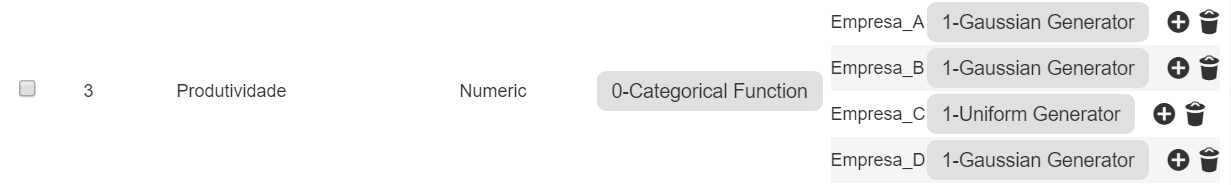
\includegraphics[width=40pc,scale=1]{figures/geradorBlocks.png}
	\end{center}
	\legend{Fonte: O autor}
\end{figure}

\section{Visualização da Base}
Nesta seção será abordado as visualizações da base de dados sintética gerada foram elaborados alguns \textit{dashboard} com objetivo de extrair informações e visualizar os indicadores das empresas  fictícias da base de dados e demonstrar a flexibilidade do protótipo.

\begin{itemize}
    \item \textbf{Proposta de Dashboard 1}:
    Na \autoref{vis_dashboard_empresas} é ilustrado a primeira proposta de \textit{dashboard}, a proposta elaborada tem como objetivo proporcionar a visualização de todos os KPIs presentes na base de dados para exploração e entendimento. A proposta é composta por 4 divisões as visualizações selecionas foram as seguintes matriz de \textit{scatterplot} para os KPIs do Financeiro,\textit{barchart} para os KPIs Clientes,\textit{parralel coordinates} para os KPIs de Processos Internos, \textit{beeswarmplot} para os KPIs  de Aprendizado e Crescimento,esses respectivos KPIs estão descritos na \autoref{tabela_indicadores}
    
    \begin{figure}[!htb]
	    \caption{\label{vis_dashboard_empresas} \textit{dashboard} gerado com a base de dados sintética criada.
        }
	\begin{center}
	    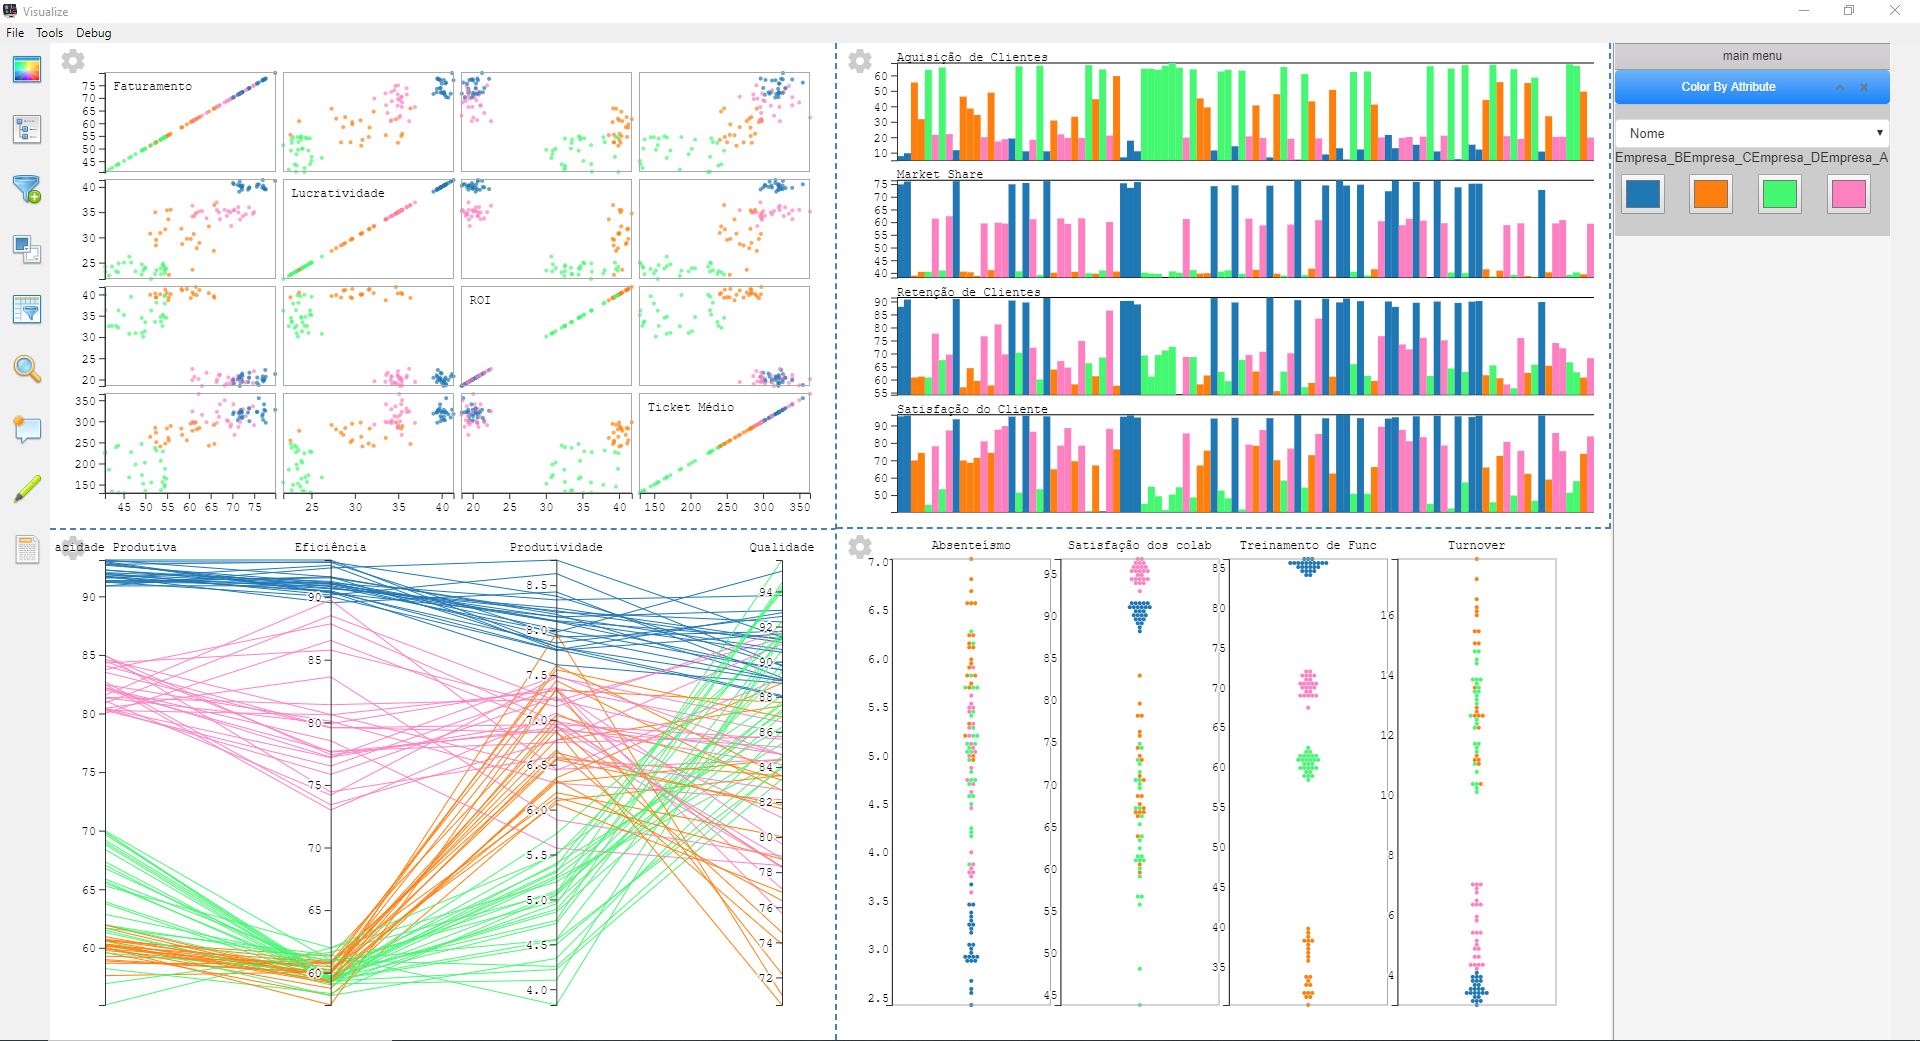
\includegraphics[width=42pc,scale=1]{figures/dash1.png}
	\end{center}
	\legend{Fonte: O autor}
    \end{figure}


    \item \textbf{Proposta de  \textit{Dashboard} 2}:
     Na \autoref{fig_dash2} pode ser verificado a segunda proposta de \textit{dashboard} gerado na ferramenta, a proposta elaborada contém duas visualizações, diferente da proposta anterior essa propõe visualizações com menos dimensões para focar em atributos específicos,fornecendo uma proposta simplificada de \textit{dashboard}, os gráficos em tela tem mesmas cores nos itens, selecionados pelo atributo "nome",a primeira visualização é um \textit{treemap} com hierarquias pelo atributo "nome" e os tamanhos organizados pela "produtividade". A segunda visualização é uma matriz \textit{scatter plot} relacionado as colunas da base de dados sintética "eficiência" e "lucratividade".
    
    \begin{figure}[!htb]
	    \caption{\label{fig_dash2} Imagem da ferramenta Blocks com um exemplo de gerador para criação da base de dados..
        }
	\begin{center}
	    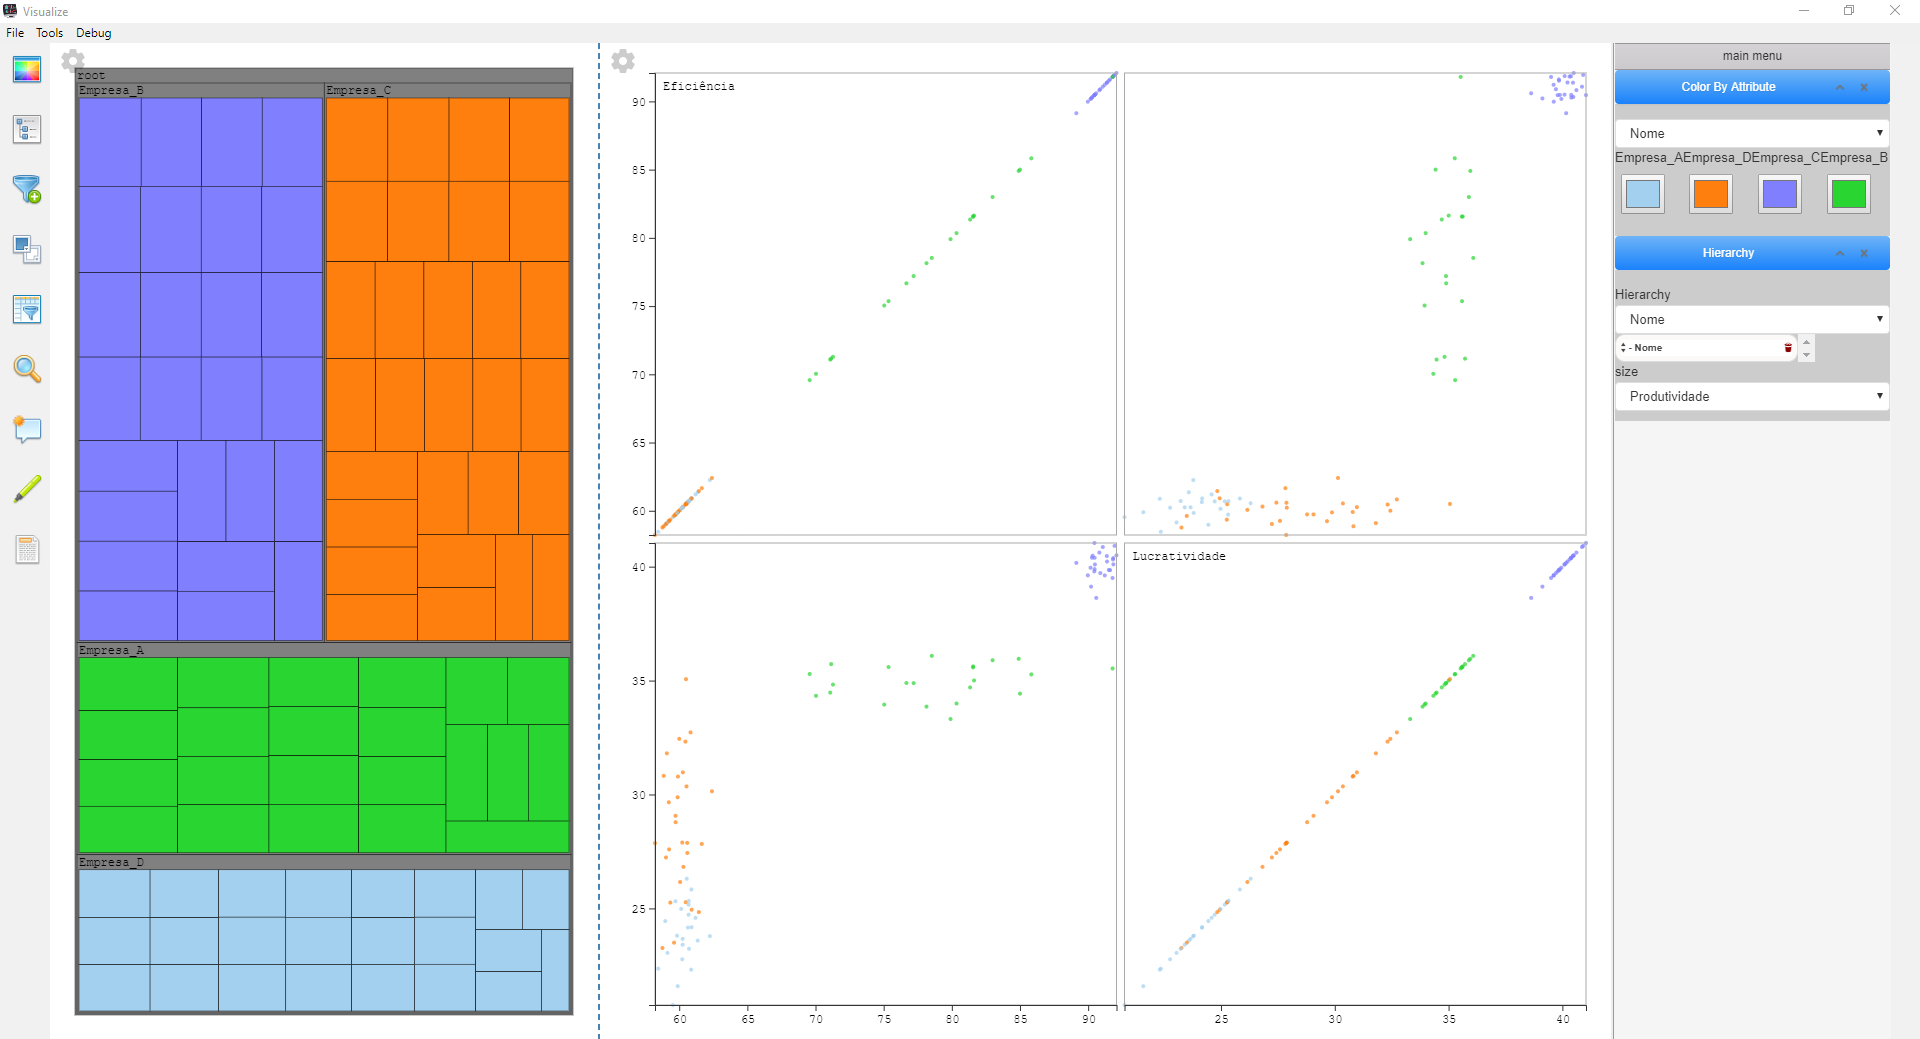
\includegraphics[width=42pc,scale=1]{figures/dash2.png}
	\end{center}
	\legend{Fonte: O autor}
    \end{figure}

    \item \textbf{Proposta de \textit{Dashboard} 3}: Na \autoref{fig_dash3} é apresentado a terceira proposta de \textit{dashboard} gerada pela ferramenta, essa proposta contém 4 visualizações com seus itens atribuídos com a mesma cor pelo atributo "nome" .A primeira um gráfico de coordenadas paralelas contendo todas as dimensões da base de dados, isso para dar um visão geral dos dados, a segunda um \textit{sunbust} com hierarquias no nome e o tamanho dos item configurado para o atributo "treinamento de funcionários", um gráfico de barras indicando a coluna "qualidade" da base de dado, e por ultimo um \textit{beeswarm plot} com na coluna de "capacidade produtiva". Essa proposta de \textit{dashboard} tem uma visão geral da base de dados,e em alguns pontos o foco em dimensões especificas como no \textit{beeswarm plot} e no gráfico de barras.
    
      \begin{figure}[!htb]
	    \caption{\label{fig_dash3} Imagem da ferramenta Blocks com um exemplo de gerador para criação da base de dados..
        }
	\begin{center}
	    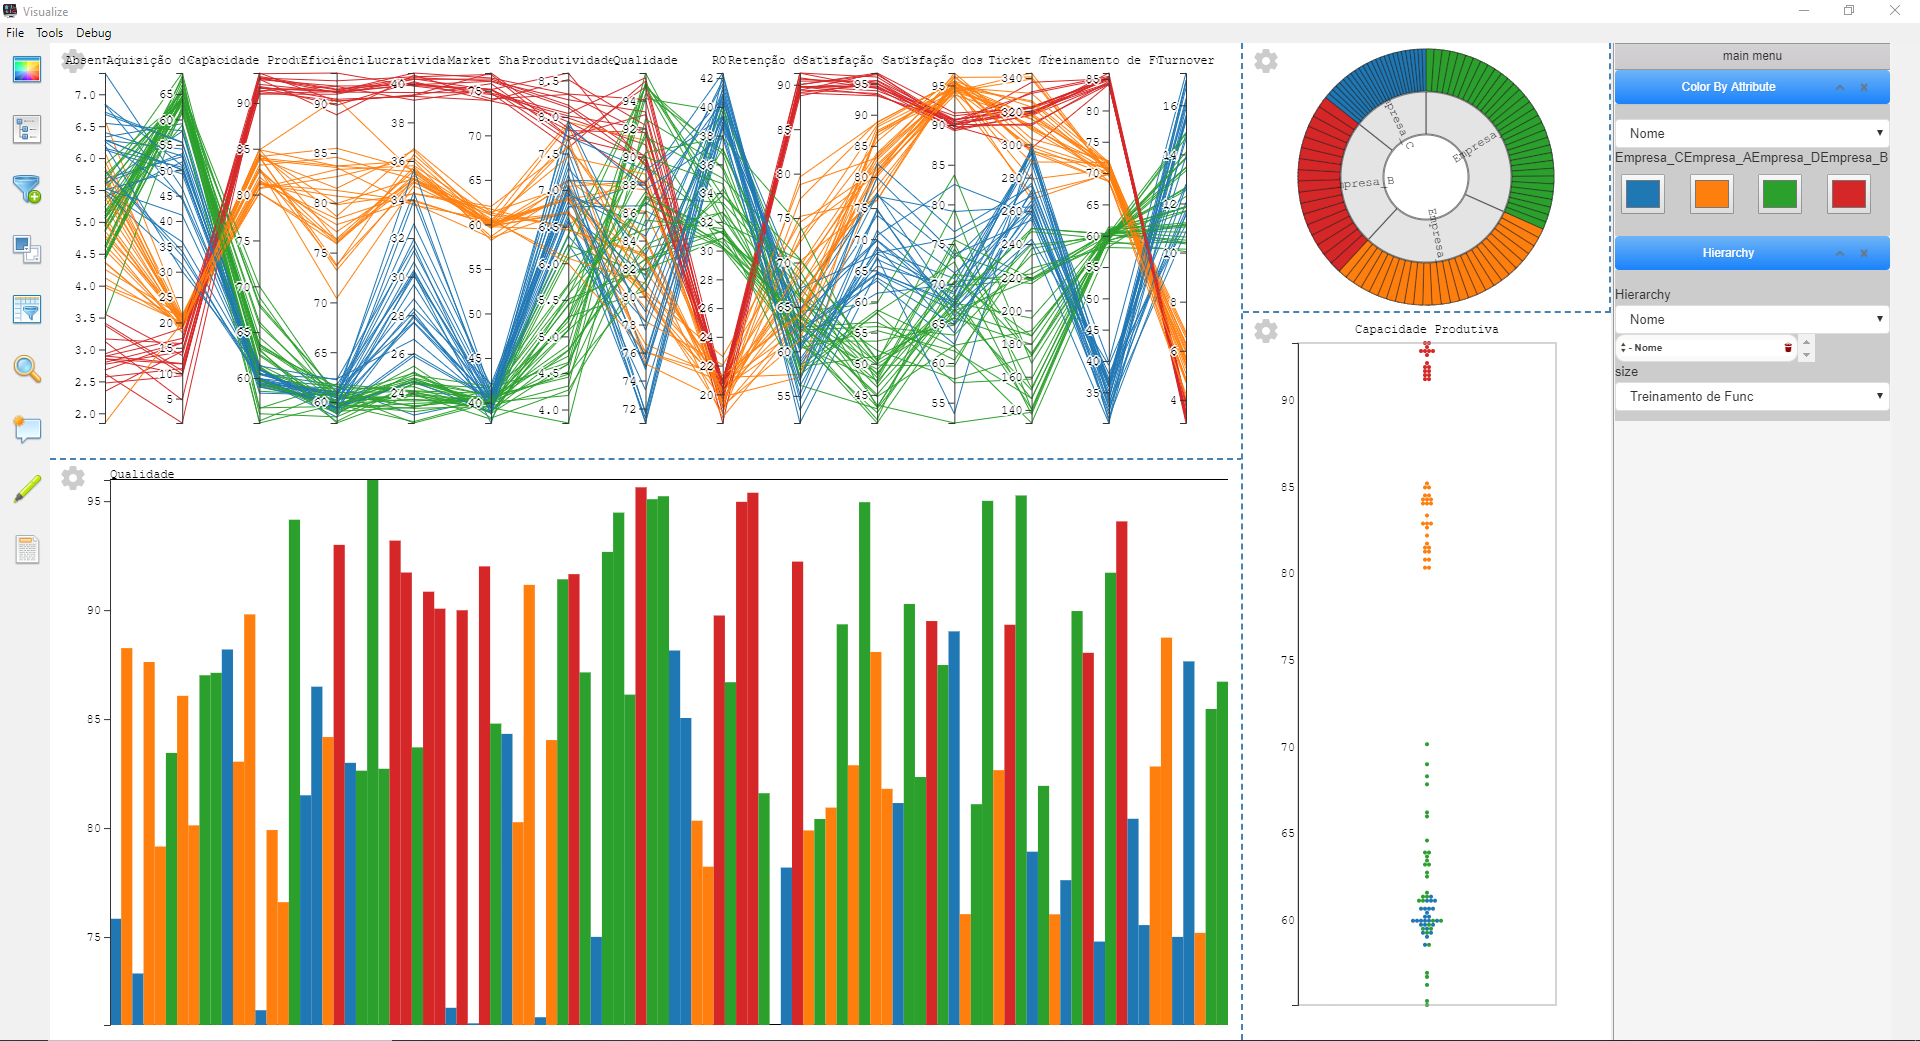
\includegraphics[width=42pc,scale=1]{figures/dash3.png}
	\end{center}
	\legend{Fonte: O autor}
    \end{figure}

\end{itemize}

\subsection{Perguntas a serem respondidas}
\begin{enumerate}
    \item Qual empresa apresenta os melhores indicadores no em relação ao Faturamento de Lucratividade?
    
     Utilizando como base o \textit{dashboard} na \autoref{vis_dashboard_empresas} as empresas "B" e "A" são as com os melhores indicadores em relação a "Faturamento" e "Lucratividade" nesse caso a empresa "B" tem os indicadores levemente melhores.
    \item Qual empresa tem pior taxa de satisfação dos colaboradores, e qual tem a melhor?
    
    Observando o \textit{beeswarm plot} na \autoref{vis_dashboard_empresas} pode ser percebido que a empresa "C" tem os piores dados em relação a indicadores de "satisfação dos colaboradores" e a empresa "A" tem os melhores indicadores para esse KPI.
    
    \item Qual empresa tem os melhores indicadores de produtividade e quais são é sua concorrente mais próxima?
    
    visualizando o \textit{treemap} na \autoref{fig_dash2} o atributo produtividade como tamanho dos item mostra que a empresa "B" tem os melhores e sua concorrente mais próxima é nesse quesito de "produtividade" é a empresa "C".
    
    \item Em relação a “capacidade produtiva” quais são as qual é a ordem de das empresa do melhor para o pior?
    
    As empresas em relação a capacidade produtiva seguem a ordem respectivamente do melhor para o pior empresa "B", "A", "C" , e "D". 
    
    \item Qual empresa tem os piores indicadores em relação a retenção de talentos e capital intelectual “Turnover” e qual os melhores?
    Seguindo a ordem as empresas com índice maior de "Turnover".O pior desempenho nesse indicador a empresa "D" entre 5\% e 10\% so pior em situação de alerta, e empresa "B" tem a melhor classificação ainda menor que 5\% definido como OK.
    
    
    
\end{enumerate}

\chapter{Considerações Finais e Trabalhos Futuros}
\label{ch:conclusao}

Nesse trabalho de conclusão de curso foi desenvolvido uma ferramenta capaz de criar \textit{dashboards} de forma interativa e incremental, desde a definição do layout das divisões até a seleção de quais visualizações estarão nas respectivas divisões. A aplicação pode gerar um conjunto de técnicas de \textit{Infovis} e fornece interações para trabalhar essas técnicas de maneira coordenada.  

As visualizações selecionadas, carregam diferentes características com possibilidades diversas para criação de diferentes \textit{dashboards} com customizações e interações, bem como a possibilidade de exportar tanto os layouts quanto as visualizações \textit{dashboads} para uso posterior pela ferramenta.

Como uma proposta de trabalho futuro pretendemos criar uma funcionalidade envolvendo aprendizado de máquina onde seja possível o próprio sistema sugerir layout de \textit{dashboard} dependendo da base de dados, com um passo de validação pelo usuário de como ficarão exibidas em tela as visualizações disponíveis. Além disso, a implementação de outras visualizações podem ser realizadas para utilização em outros contextos como \textit{piechart}, \textit{wordcloud}, \textit{heatmap} e \textit{linechart}.

Outro trabalho futuro é a migração dessa aplicação \textit{desktop} para web, ficando assim disponível em servidor com domínio para acesso dos usuários e também realizar integração com banco de dados SQL. Estando em um ambiente online a aplicação terá um novo leque de possibilidades como um módulo multiusuário, permitindo vários usuários acessarem um ambiente colaborativo online e reativo para modelagem de um \textit{dashboard} ou exploração e análise do mesmo. Para realização dessas propostas além da migração para web será necessário um módulo de gerenciamento e permissões de usuários em tempo real no ambiente da web.

Finalizando é necessário avaliar a aplicação com usuários experientes e inexperientes, propondo tarefas de visualização de dados para avaliar a usabilidade da ferramenta e identificar novas necessidades em relação aos \textit{dashboads}, da mesma forma avaliar os pontos positivos e negativos.





% % ----------------------------------------------------------
% % Introdução (exemplo de capítulo sem numeração, mas presente no Sumário)
% % ----------------------------------------------------------
% \chapter{Introdução}
% % ----------------------------------------------------------


% Este documento e seu código-fonte são exemplos de referência de uso da classe
% \textsf{abntex2} e do pacote \textsf{abntex2cite}. O documento 
% exemplifica a elaboração de trabalho acadêmico (tese, dissertação e outros do
% gênero) produzido conforme a ABNT NBR 14724:2011 \emph{Informação e documentação
% - Trabalhos acadêmicos - Apresentação}.

% A expressão ``Modelo Canônico'' é utilizada para indicar que \abnTeX\ não é
% modelo específico de nenhuma universidade ou instituição, mas que implementa tão
% somente os requisitos das normas da ABNT. Uma lista completa das normas
% observadas pelo \abnTeX\ é apresentada em \cite{abntex2classe}.

% Sinta-se convidado a participar do projeto \abnTeX! Acesse o site do projeto em
% \url{http://www.abntex.net.br/}. Também fique livre para conhecer,
% estudar, alterar e redistribuir o trabalho do \abnTeX, desde que os arquivos
% modificados tenham seus nomes alterados e que os créditos sejam dados aos
% autores originais, nos termos da ``The \LaTeX\ Project Public
% License''\footnote{\url{http://www.latex-project.org/lppl.txt}}.

% Encorajamos que sejam realizadas customizações específicas deste exemplo para
% universidades e outras instituições --- como capas, folha de aprovação, etc.
% Porém, recomendamos que ao invés de se alterar diretamente os arquivos do
% \abnTeX, distribua-se arquivos com as respectivas customizações.
% Isso permite que futuras versões do \abnTeX~não se tornem automaticamente
% incompatíveis com as customizações promovidas. Consulte
% \cite{abntex2-wiki-como-customizar} para mais informações.

% Este documento deve ser utilizado como complemento dos manuais do \abnTeX\ 
% \cite{abntex2classe,abntex2cite,abntex2cite-alf} e da classe \textsf{memoir}
% \cite{memoir}. 

% Esperamos, sinceramente, que o \abnTeX\ aprimore a qualidade do trabalho que
% você produzirá, de modo que o principal esforço seja concentrado no principal:
% na contribuição científica.

% Equipe \abnTeX 

% Lauro César Araujo

% ---
% Capitulo com exemplos de comandos inseridos de arquivo externo 
% ---
% %% abtex2-modelo-include-comandos.tex, v-1.9.7 laurocesar
%% Copyright 2012-2018 by abnTeX2 group at http://www.abntex.net.br/ 
%%
%% This work may be distributed and/or modified under the
%% conditions of the LaTeX Project Public License, either version 1.3
%% of this license or (at your option) any later version.
%% The latest version of this license is in
%%   http://www.latex-project.org/lppl.txt
%% and version 1.3 or later is part of all distributions of LaTeX
%% version 2005/12/01 or later.
%%
%% This work has the LPPL maintenance status `maintained'.
%% 
%% The Current Maintainer of this work is the abnTeX2 team, led
%% by Lauro César Araujo. Further information are available on 
%% http://www.abntex.net.br/
%%
%% This work consists of the files abntex2-modelo-include-comandos.tex
%% and abntex2-modelo-img-marca.pdf
%%

% ---
% Este capítulo, utilizado por diferentes exemplos do abnTeX2, ilustra o uso de
% comandos do abnTeX2 e de LaTeX.
% ---
 
\chapter{Resultados de comandos}\label{cap_exemplos}

Isto é uma sinopse de capítulo. A ABNT não traz nenhuma
normatização a respeito desse tipo de resumo, que é mais comum em romances 
e livros técnicos.

% ---
\section{Codificação dos arquivos: UTF8}
% ---

A codificação de todos os arquivos do \abnTeX\ é \texttt{UTF8}. É necessário que
você utilize a mesma codificação nos documentos que escrever, inclusive nos
arquivos de base bibliográficas |.bib|.

% ---
\section{Citações diretas}
\label{sec-citacao}
% ---

\index{citações!diretas}Utilize o ambiente \texttt{citacao} para incluir
citações diretas com mais de três linhas:

\begin{citacao}
As citações diretas, no texto, com mais de três linhas, devem ser
destacadas com recuo de 4 cm da margem esquerda, com letra menor que a do texto
utilizado e sem as aspas. No caso de documentos datilografados, deve-se
observar apenas o recuo \cite[5.3]{NBR10520:2002}.
\end{citacao}

Use o ambiente assim:

\begin{verbatim}
\begin{citacao}
As citações diretas, no texto, com mais de três linhas [...] deve-se observar
apenas o recuo \cite[5.3]{NBR10520:2002}.
\end{citacao}
\end{verbatim}

O ambiente \texttt{citacao} pode receber como parâmetro opcional um nome de
idioma previamente carregado nas opções da classe (\autoref{sec-hifenizacao}). Nesse
caso, o texto da citação é automaticamente escrito em itálico e a hifenização é
ajustada para o idioma selecionado na opção do ambiente. Por exemplo:

\begin{verbatim}
\begin{citacao}[english]
Text in English language in italic with correct hyphenation.
\end{citacao}
\end{verbatim}

Tem como resultado:

\begin{citacao}[english]
Text in English language in italic with correct hyphenation.
\end{citacao}

\index{citações!simples}Citações simples, com até três linhas, devem ser
incluídas com aspas. Observe que em \LaTeX as aspas iniciais são diferentes das
finais: ``Amor é fogo que arde sem se ver''.

% ---
\section{Notas de rodapé}
% ---

As notas de rodapé são detalhadas pela NBR 14724:2011 na seção 5.2.1\footnote{As
notas devem ser digitadas ou datilografadas dentro das margens, ficando
separadas do texto por um espaço simples de entre as linhas e por filete de 5
cm, a partir da margem esquerda. Devem ser alinhadas, a partir da segunda linha
da mesma nota, abaixo da primeira letra da primeira palavra, de forma a destacar
o expoente, sem espaço entre elas e com fonte menor
\cite{NBR14724:2011}}\footnote{Caso uma série de notas sejam
criadas sequencialmente, o \abnTeX\ instrui o \LaTeX\ para que uma vírgula seja
colocada após cada número do expoente que indica a nota de rodapé no corpo do
texto.}\footnote{Verifique se os números do expoente possuem uma vírgula para
dividi-los no corpo do texto.}. 


% ---
\section{Tabelas}
% ---

\index{tabelas}A \autoref{tab-nivinv} é um exemplo de tabela construída em
\LaTeX.

\begin{table}[htb]
\ABNTEXfontereduzida
\caption[Níveis de investigação]{Níveis de investigação.}
\label{tab-nivinv}
\begin{tabular}{p{2.6cm}|p{6.0cm}|p{2.25cm}|p{3.40cm}}
  %\hline
  \textbf{Nível de Investigação} & \textbf{Insumos}  & \textbf{Sistemas de Investigação}  & \textbf{Produtos}  \\
    \hline
    Meta-nível & Filosofia\index{filosofia} da Ciência  & Epistemologia &
    Paradigma  \\
    \hline
    Nível do objeto & Paradigmas do metanível e evidências do nível inferior &
    Ciência  & Teorias e modelos \\
    \hline
    Nível inferior & Modelos e métodos do nível do objeto e problemas do nível inferior & Prática & Solução de problemas  \\
  % \hline
\end{tabular}
\legend{Fonte: \cite{van86}}
\end{table}

Já a \autoref{tabela-ibge} apresenta uma tabela criada conforme o padrão do
\cite{ibge1993} requerido pelas normas da ABNT para documentos técnicos e
acadêmicos.

\begin{table}[htb]
\IBGEtab{%
  \caption{Um Exemplo de tabela alinhada que pode ser longa
  ou curta, conforme padrão IBGE.}%
  \label{tabela-ibge}
}{%
  \begin{tabular}{ccc}
  \toprule
  Nome & Nascimento & Documento \\
  \midrule \midrule
  Maria da Silva & 11/11/1111 & 111.111.111-11 \\
  \midrule 
  João Souza & 11/11/2111 & 211.111.111-11 \\
  \midrule 
  Laura Vicuña & 05/04/1891 & 3111.111.111-11 \\
  \bottomrule
\end{tabular}%
}{%
  \fonte{Produzido pelos autores.}%
  \nota{Esta é uma nota, que diz que os dados são baseados na
  regressão linear.}%
  \nota[Anotações]{Uma anotação adicional, que pode ser seguida de várias
  outras.}%
  }
\end{table}


% ---
\section{Figuras}
% ---

\index{figuras}Figuras podem ser criadas diretamente em \LaTeX,
como o exemplo da \autoref{fig_circulo}.

\begin{figure}[htb]
    \label{fig_circulo}
	\caption{Aliquam arcu neque, ornarein, ullamcorper quis, commodo eu, libero. Fusce sagittis erat at erat tristiquemollis. Maecenas sapien libero, molestie et, lobortis in, sodales eget, dui. Morbiultrices rutrum lorem. Nam elementum ullamcorper leo. Morbi dui. Aliquamsagittis. Nunc placerat. Pellentesque tristique sodales est. Maecenas imperdietlacinia velit. Cras non urna. Morbi eros pede, suscipit ac, varius vel, egestasnon, eros. Praesent malesuada, diam id pretium elementum, eros sem dictumtortor, vel consectetuer odio sem sed wisi.}
	\begin{center}
	    \setlength{\unitlength}{5cm}
		\begin{picture}(1,1)
		\put(0,0){\line(0,1){1}}
		\put(0,0){\line(1,0){1}}
		\put(0,0){\line(1,1){1}}
		\put(0,0){\line(1,2){.5}}
		\put(0,0){\line(1,3){.3333}}
		\put(0,0){\line(1,4){.25}}
		\put(0,0){\line(1,5){.2}}
		\put(0,0){\line(1,6){.1667}}
		\put(0,0){\line(2,1){1}}
		\put(0,0){\line(2,3){.6667}}
		\put(0,0){\line(2,5){.4}}
		\put(0,0){\line(3,1){1}}
		\put(0,0){\line(3,2){1}}
		\put(0,0){\line(3,4){.75}}
		\put(0,0){\line(3,5){.6}}
		\put(0,0){\line(4,1){1}}
		\put(0,0){\line(4,3){1}}
		\put(0,0){\line(4,5){.8}}
		\put(0,0){\line(5,1){1}}
		\put(0,0){\line(5,2){1}}
		\put(0,0){\line(5,3){1}}
		\put(0,0){\line(5,4){1}}
		\put(0,0){\line(5,6){.8333}}
		\put(0,0){\line(6,1){1}}
		\put(0,0){\line(6,5){1}}
		\end{picture}
	\end{center}
	\legend{Fonte: os autores}
\end{figure}

Ou então figuras podem ser incorporadas de arquivos externos, como é o caso da
\autoref{fig_grafico}. Se a figura que for incluída se tratar de um diagrama, um
gráfico ou uma ilustração que você mesmo produza, priorize o uso de imagens
vetoriais no formato PDF. Com isso, o tamanho do arquivo final do trabalho será
menor, e as imagens terão uma apresentação melhor, principalmente quando
impressas, uma vez que imagens vetorias são perfeitamente escaláveis para
qualquer dimensão. Nesse caso, se for utilizar o Microsoft Excel para produzir
gráficos, ou o Microsoft Word para produzir ilustrações, exporte-os como PDF e
os incorpore ao documento conforme o exemplo abaixo. No entanto, para manter a
coerência no uso de software livre (já que você está usando \LaTeX e \abnTeX),
teste a ferramenta \textsf{InkScape}\index{InkScape}
(\url{http://inkscape.org/}). Ela é uma excelente opção de código-livre para
produzir ilustrações vetoriais, similar ao CorelDraw\index{CorelDraw} ou ao Adobe
Illustrator\index{Adobe Illustrator}. De todo modo, caso não seja possível
utilizar arquivos de imagens como PDF, utilize qualquer outro formato, como
JPEG, GIF, BMP, etc. Nesse caso, você pode tentar aprimorar as imagens
incorporadas com o software livre \textsf{Gimp}\index{Gimp}
(\url{http://www.gimp.org/}). Ele é uma alternativa livre ao Adobe
Photoshop\index{Adobe Photoshop}.

\begin{figure}[htb]
	\caption{\label{fig_grafico}Gráfico produzido em Excel e salvo como PDF}
	\begin{center}
	    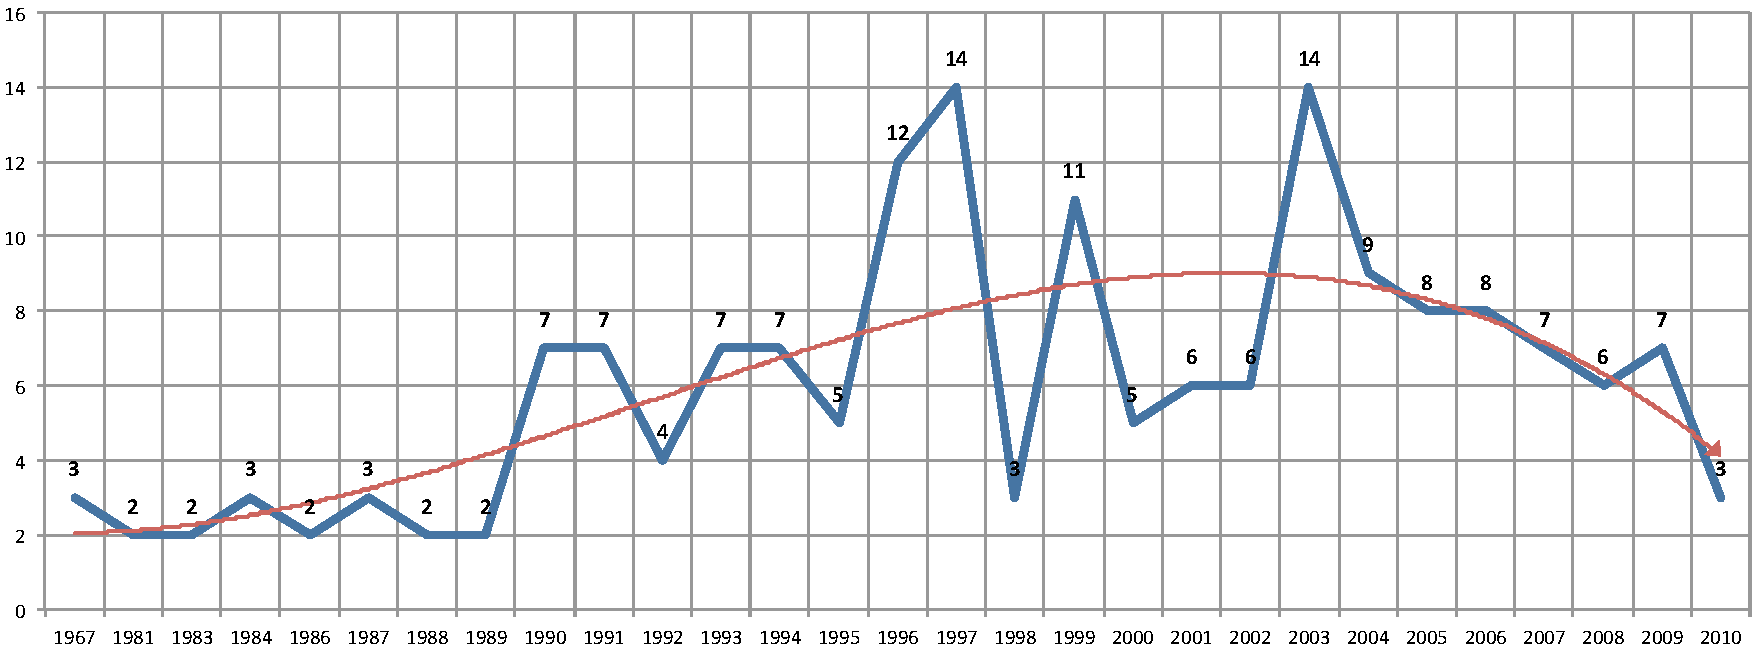
\includegraphics[scale=0.5]{abntex2-modelo-img-grafico.pdf}
	\end{center}
	\legend{Fonte: \cite{araujo2012}}
\end{figure}

% ---
\subsection{Figuras em \emph{minipages}}
% ---

\emph{Minipages} são usadas para inserir textos ou outros elementos em quadros
com tamanhos e posições controladas. Veja o exemplo da
\autoref{fig_minipage_imagem1} e da \autoref{fig_minipage_grafico2}.

\begin{figure}[htb]
 \label{teste}
 \centering
  \begin{minipage}{0.4\textwidth}
    \centering
    \caption{Imagem 1 da minipage} \label{fig_minipage_imagem1}
    
\includegraphics[scale=0.9]{abntex2-modelo-img-marca.pdf}
    \legend{Fonte: Produzido pelos autores}
  \end{minipage}
  \hfill
  \begin{minipage}{0.4\textwidth}
    \centering
    \caption{Grafico 2 da minipage} \label{fig_minipage_grafico2}
    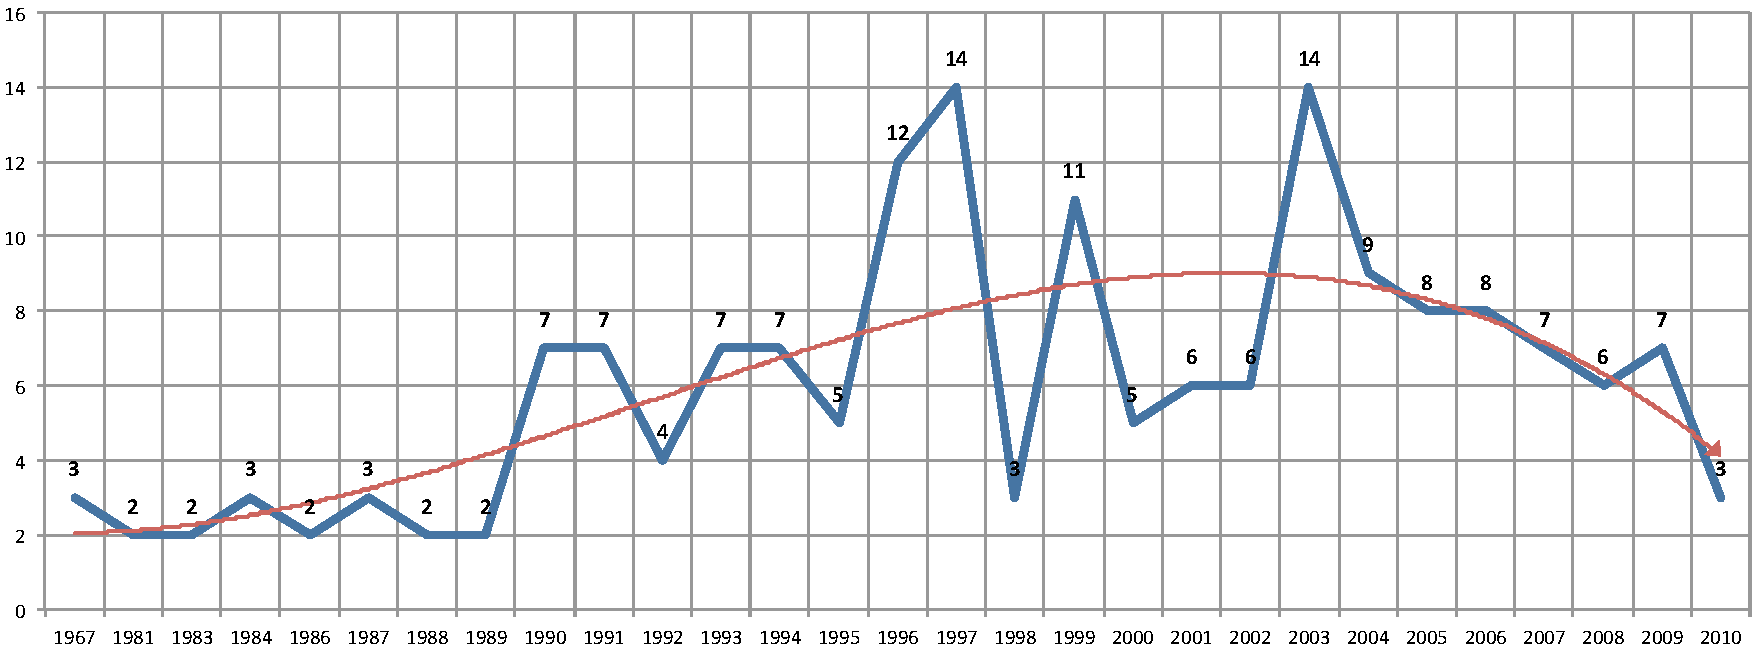
\includegraphics[scale=0.2]{abntex2-modelo-img-grafico.pdf}
    \legend{Fonte: \cite{araujo2012}}
  \end{minipage}
\end{figure}

Observe que, segundo a \cite{NBR14724:2011}, seções 4.2.1.10 e 5.8, as
ilustrações devem sempre ter numeração contínua e única em todo o documento:

\begin{citacao}
Qualquer que seja o tipo de ilustração, sua identificação aparece na parte
superior, precedida da palavra designativa (desenho, esquema, fluxograma,
fotografia, gráfico, mapa, organograma, planta, quadro, retrato, figura,
imagem, entre outros), seguida de seu número de ordem de ocorrência no texto,
em algarismos arábicos, travessão e do respectivo título. Após a ilustração, na
parte inferior, indicar a fonte consultada (elemento obrigatório, mesmo que
seja produção do próprio autor), legenda, notas e outras informações
necessárias à sua compreensão (se houver). A ilustração deve ser citada no
texto e inserida o mais próximo possível do trecho a que se
refere. \cite[seções 5.8]{NBR14724:2011}
\end{citacao}

% ---
\section{Expressões matemáticas}
% ---

\index{expressões matemáticas}Use o ambiente \texttt{equation} para escrever
expressões matemáticas numeradas:

\begin{equation}
  \forall x \in X, \quad \exists \: y \leq \epsilon
\end{equation}

Escreva expressões matemáticas entre \$ e \$, como em $ \lim_{x \to \infty}
\exp(-x) = 0 $, para que fiquem na mesma linha.

Também é possível usar colchetes para indicar o início de uma expressão
matemática que não é numerada.

\[
\left|\sum_{i=1}^n a_ib_i\right|
\le
\left(\sum_{i=1}^n a_i^2\right)^{1/2}
\left(\sum_{i=1}^n b_i^2\right)^{1/2}
\]

Consulte mais informações sobre expressões matemáticas em
\url{https://github.com/abntex/abntex2/wiki/Referencias}.

% ---
\section{Enumerações: alíneas e subalíneas}
% ---

\index{alíneas}\index{subalíneas}\index{incisos}Quando for necessário enumerar
os diversos assuntos de uma seção que não possua título, esta deve ser
subdividida em alíneas \cite[4.2]{NBR6024:2012}:

\begin{alineas}

  \item os diversos assuntos que não possuam título próprio, dentro de uma mesma
  seção, devem ser subdivididos em alíneas; 
  
  \item o texto que antecede as alíneas termina em dois pontos;
  \item as alíneas devem ser indicadas alfabeticamente, em letra minúscula,
  seguida de parêntese. Utilizam-se letras dobradas, quando esgotadas as
  letras do alfabeto;

  \item as letras indicativas das alíneas devem apresentar recuo em relação à
  margem esquerda;

  \item o texto da alínea deve começar por letra minúscula e terminar em
  ponto-e-vírgula, exceto a última alínea que termina em ponto final;

  \item o texto da alínea deve terminar em dois pontos, se houver subalínea;

  \item a segunda e as seguintes linhas do texto da alínea começa sob a
  primeira letra do texto da própria alínea;
  
  \item subalíneas \cite[4.3]{NBR6024:2012} devem ser conforme as alíneas a
  seguir:

  \begin{alineas}
     \item as subalíneas devem começar por travessão seguido de espaço;

     \item as subalíneas devem apresentar recuo em relação à alínea;

     \item o texto da subalínea deve começar por letra minúscula e terminar em
     ponto-e-vírgula. A última subalínea deve terminar em ponto final, se não
     houver alínea subsequente;

     \item a segunda e as seguintes linhas do texto da subalínea começam sob a
     primeira letra do texto da própria subalínea.
  \end{alineas}
  
  \item no \abnTeX\ estão disponíveis os ambientes \texttt{incisos} e
  \texttt{subalineas}, que em suma são o mesmo que se criar outro nível de
  \texttt{alineas}, como nos exemplos à seguir:
  
  \begin{incisos}
    \item \textit{Um novo inciso em itálico};
  \end{incisos}
  
  \item Alínea em \textbf{negrito}:
  
  \begin{subalineas}
    \item \textit{Uma subalínea em itálico};
    \item \underline{\textit{Uma subalínea em itálico e sublinhado}}; 
  \end{subalineas}
  
  \item Última alínea com \emph{ênfase}.
  
\end{alineas}

% ---
\section{Espaçamento entre parágrafos e linhas}
% ---

\index{espaçamento!dos parágrafos}O tamanho do parágrafo, espaço entre a margem
e o início da frase do parágrafo, é definido por:

\begin{verbatim}
  \setlength{\parindent}{1.3cm}
\end{verbatim}

\index{espaçamento!do primeiro parágrafo}Por padrão, não há espaçamento no
primeiro parágrafo de cada início de divisão do documento
(\autoref{sec-divisoes}). Porém, você pode definir que o primeiro parágrafo
também seja indentado, como é o caso deste documento. Para isso, apenas inclua o
pacote \textsf{indentfirst} no preâmbulo do documento:

\begin{verbatim}
  \usepackage{indentfirst}      % Indenta o primeiro parágrafo de cada seção.
\end{verbatim}

\index{espaçamento!entre os parágrafos}O espaçamento entre um parágrafo e outro
pode ser controlado por meio do comando:

\begin{verbatim}
  \setlength{\parskip}{0.2cm}  % tente também \onelineskip
\end{verbatim}

\index{espaçamento!entre as linhas}O controle do espaçamento entre linhas é
definido por:

\begin{verbatim}
  \OnehalfSpacing       % espaçamento um e meio (padrão); 
  \DoubleSpacing        % espaçamento duplo
  \SingleSpacing        % espaçamento simples	
\end{verbatim}

Para isso, também estão disponíveis os ambientes:

\begin{verbatim}
  \begin{SingleSpace} ...\end{SingleSpace}
  \begin{Spacing}{hfactori} ... \end{Spacing}
  \begin{OnehalfSpace} ... \end{OnehalfSpace}
  \begin{OnehalfSpace*} ... \end{OnehalfSpace*}
  \begin{DoubleSpace} ... \end{DoubleSpace}
  \begin{DoubleSpace*} ... \end{DoubleSpace*} 
\end{verbatim}

Para mais informações, consulte \cite{memoir}.

% ---
\section{Inclusão de outros arquivos}\label{sec-include}
% ---

É uma boa prática dividir o seu documento em diversos arquivos, e não
apenas escrever tudo em um único. Esse recurso foi utilizado neste
documento. Para incluir diferentes arquivos em um arquivo principal,
de modo que cada arquivo incluído fique em uma página diferente, utilize o
comando:

\begin{verbatim}
  \include{documento-a-ser-incluido}      % sem a extensão .tex
\end{verbatim}

Para incluir documentos sem quebra de páginas, utilize:

\begin{verbatim}
  \input{documento-a-ser-incluido}      % sem a extensão .tex
\end{verbatim}

% ---
\section{Compilar o documento \LaTeX}
% ---

Geralmente os editores \LaTeX, como o
TeXlipse\footnote{\url{http://texlipse.sourceforge.net/}}, o
Texmaker\footnote{\url{http://www.xm1math.net/texmaker/}}, entre outros,
compilam os documentos automaticamente, de modo que você não precisa se
preocupar com isso.

No entanto, você pode compilar os documentos \LaTeX usando os seguintes
comandos, que devem ser digitados no \emph{Prompt de Comandos} do Windows ou no
\emph{Terminal} do Mac ou do Linux:

\begin{verbatim}
  pdflatex ARQUIVO_PRINCIPAL.tex
  bibtex ARQUIVO_PRINCIPAL.aux
  makeindex ARQUIVO_PRINCIPAL.idx 
  makeindex ARQUIVO_PRINCIPAL.nlo -s nomencl.ist -o ARQUIVO_PRINCIPAL.nls
  pdflatex ARQUIVO_PRINCIPAL.tex
  pdflatex ARQUIVO_PRINCIPAL.tex
\end{verbatim}

% ---
\section{Remissões internas}
% ---

Ao nomear a \autoref{tab-nivinv} e a \autoref{fig_circulo}, apresentamos um
exemplo de remissão interna, que também pode ser feita quando indicamos o
\autoref{cap_exemplos}, que tem o nome \emph{\nameref{cap_exemplos}}. O número
do capítulo indicado é \ref{cap_exemplos}, que se inicia à
\autopageref{cap_exemplos}\footnote{O número da página de uma remissão pode ser
obtida também assim:
\pageref{cap_exemplos}.}.
Veja a \autoref{sec-divisoes} para outros exemplos de remissões internas entre
seções, subseções e subsubseções.

O código usado para produzir o texto desta seção é:

\begin{verbatim}
Ao nomear a \autoref{tab-nivinv} e a \autoref{fig_circulo}, apresentamos um
exemplo de remissão interna, que também pode ser feita quando indicamos o
\autoref{cap_exemplos}, que tem o nome \emph{\nameref{cap_exemplos}}. O número
do capítulo indicado é \ref{cap_exemplos}, que se inicia à
\autopageref{cap_exemplos}\footnote{O número da página de uma remissão pode ser
obtida também assim:
\pageref{cap_exemplos}.}.
Veja a \autoref{sec-divisoes} para outros exemplos de remissões internas entre
seções, subseções e subsubseções.
\end{verbatim}

% ---
\section{Divisões do documento: seção}\label{sec-divisoes}
% ---

Esta seção testa o uso de divisões de documentos. Esta é a
\autoref{sec-divisoes}. Veja a \autoref{sec-divisoes-subsection}.

\subsection{Divisões do documento: subseção}\label{sec-divisoes-subsection}

Isto é uma subseção. Veja a \autoref{sec-divisoes-subsubsection}, que é uma
\texttt{subsubsection} do \LaTeX, mas é impressa chamada de ``subseção'' porque
no Português não temos a palavra ``subsubseção''.

\subsubsection{Divisões do documento: subsubseção}
\label{sec-divisoes-subsubsection}

Isto é uma subsubseção.

\subsubsection{Divisões do documento: subsubseção}

Isto é outra subsubseção.

\subsection{Divisões do documento: subseção}\label{sec-exemplo-subsec}

Isto é uma subseção.

\subsubsection{Divisões do documento: subsubseção}

Isto é mais uma subsubseção da \autoref{sec-exemplo-subsec}.


\subsubsubsection{Esta é uma subseção de quinto
nível}\label{sec-exemplo-subsubsubsection}

Esta é uma seção de quinto nível. Ela é produzida com o seguinte comando:

\begin{verbatim}
\subsubsubsection{Esta é uma subseção de quinto
nível}\label{sec-exemplo-subsubsubsection}
\end{verbatim}

\subsubsubsection{Esta é outra subseção de quinto nível}\label{sec-exemplo-subsubsubsection-outro}

Esta é outra seção de quinto nível.


\paragraph{Este é um parágrafo numerado}\label{sec-exemplo-paragrafo}

Este é um exemplo de parágrafo nomeado. Ele é produzida com o comando de
parágrafo:

\begin{verbatim}
\paragraph{Este é um parágrafo nomeado}\label{sec-exemplo-paragrafo}
\end{verbatim}

A numeração entre parágrafos numeradaos e subsubsubseções são contínuas.

\paragraph{Esta é outro parágrafo numerado}\label{sec-exemplo-paragrafo-outro}

Esta é outro parágrafo nomeado.

% ---
\section{Este é um exemplo de nome de seção longo. Ele deve estar
alinhado à esquerda e a segunda e demais linhas devem iniciar logo abaixo da
primeira palavra da primeira linha}
% ---

Isso atende à norma \cite{NBR14724:2011} seções de 5.2.2 a 5.2.4 
 e \cite{NBR6024:2012} seções de 3.1 a 3.8.

% ---
\section{Diferentes idiomas e hifenizações}
\label{sec-hifenizacao}
% ---

Para usar hifenizações de diferentes idiomas, inclua nas opções do documento o
nome dos idiomas que o seu texto contém. Por exemplo (para melhor
visualização, as opções foram quebras em diferentes linhas):

\begin{verbatim}
\documentclass[
	12pt,
	openright,
	twoside,
	a4paper,
	english,
	french,
	spanish,
	brazil
	]{abntex2}
\end{verbatim}

O idioma português-brasileiro (\texttt{brazil}) é incluído automaticamente pela
classe \textsf{abntex2}. Porém, mesmo assim a opção \texttt{brazil} deve ser
informada como a última opção da classe para que todos os pacotes reconheçam o
idioma. Vale ressaltar que a última opção de idioma é a utilizada por padrão no
documento. Desse modo, caso deseje escrever um texto em inglês que tenha
citações em português e em francês, você deveria usar o preâmbulo como abaixo:

\begin{verbatim}
\documentclass[
	12pt,
	openright,
	twoside,
	a4paper,
	french,
	brazil,
	english
	]{abntex2}
\end{verbatim}

A lista completa de idiomas suportados, bem como outras opções de hifenização,
estão disponíveis em \cite{babel} p. 5-6.

Exemplo de hifenização em inglês\footnote{Extraído de:
\url{http://en.wikibooks.org/wiki/LaTeX/Internationalization}}:

\begin{otherlanguage*}{english}
\textit{Text in English language. This environment switches all language-related
definitions, like the language specific names for figures, tables etc. to the other
language. The starred version of this environment typesets the main text
according to the rules of the other language, but keeps the language specific
string for ancillary things like figures, in the main language of the document.
The environment hyphenrules switches only the hyphenation patterns used; it can
also be used to disallow hyphenation by using the language name
`nohyphenation'.}
\end{otherlanguage*}

Exemplo de hifenização em francês\footnote{Extraído de:
\url{http://bigbrowser.blog.lemonde.fr/2013/02/17/tu-ne-tweeteras-point-le-vatican-interdit-aux-cardinaux-de-tweeter-pendant-le-conclave/}}:

\begin{otherlanguage*}{french}
\textit{Texte en français. Pas question que Twitter ne vienne faire une
concurrence déloyale à la traditionnelle fumée blanche qui marque l'élection
d'un nouveau pape. Pour éviter toute fuite précoce, le Vatican a donc pris un
peu d'avance, et a déjà interdit aux cardinaux qui prendront part au vote
d'utiliser le réseau social, selon Catholic News Service. Une mesure valable
surtout pour les neuf cardinaux – sur les 117 du conclave – pratiquants très
actifs de Twitter, qui auront interdiction pendant toute la période de se
connecter à leur compte.}
\end{otherlanguage*}

Pequeno texto em espanhol\footnote{Extraído de:
\url{http://internacional.elpais.com/internacional/2013/02/17/actualidad/1361102009_913423.html}}:

\foreignlanguage{spanish}{\textit{Decenas de miles de personas ovacionan al pontífice en su
penúltimo ángelus dominical, el primero desde que anunciase su renuncia. El Papa se
centra en la crítica al materialismo}}.

O idioma geral do texto por ser alterado como no exemplo seguinte:

\begin{verbatim}
  \selectlanguage{english}
\end{verbatim}

Isso altera automaticamente a hifenização e todos os nomes constantes de
referências do documento para o idioma inglês. Consulte o manual da classe
\cite{abntex2classe} para obter orientações adicionais sobre internacionalização de
documentos produzidos com \abnTeX.

A \autoref{sec-citacao} descreve o ambiente \texttt{citacao} que pode receber
como parâmetro um idioma a ser usado na citação.

% ---
\section{Consulte o manual da classe \textsf{abntex2}}
% ---

Consulte o manual da classe \textsf{abntex2} \cite{abntex2classe} para uma
referência completa das macros e ambientes disponíveis. 

Além disso, o manual possui informações adicionais sobre as normas ABNT
observadas pelo \abnTeX\ e considerações sobre eventuais requisitos específicos
não atendidos, como o caso da \cite{NBR14724:2011} seção 5.2.2, que
especifica o espaçamento entre os capítulos e o início do texto, regra
propositalmente não atendida pelo presente modelo.

% ---
\section{Referências bibliográficas}
% ---

A formatação das referências bibliográficas conforme as regras da ABNT são um
dos principais objetivos do \abnTeX. Consulte os manuais
\cite{abntex2cite} e \cite{abntex2cite-alf} para obter informações
sobre como utilizar as referências bibliográficas.

%-
\subsection{Acentuação de referências bibliográficas}
%-

Normalmente não há problemas em usar caracteres acentuados em arquivos
bibliográficos (\texttt{*.bib}). Porém, como as regras da ABNT fazem uso quase
abusivo da conversão para letras maiúsculas, é preciso observar o modo como se
escreve os nomes dos autores. Na ~\autoref{tabela-acentos} você encontra alguns
exemplos das conversões mais importantes. Preste atenção especial para `ç' e `í'
que devem estar envoltos em chaves. A regra geral é sempre usar a acentuação
neste modo quando houver conversão para letras maiúsculas.

\begin{table}[htbp]
\caption{Tabela de conversão de acentuação.}
\label{tabela-acentos}

\begin{center}
\begin{tabular}{ll}\hline\hline
acento & \textsf{bibtex}\\
à á ã & \verb+\`a+ \verb+\'a+ \verb+\~a+\\
í & \verb+{\'\i}+\\
ç & \verb+{\c c}+\\
\hline\hline
\end{tabular}
\end{center}
\end{table}


% ---
\section{Precisa de ajuda?}
% ---

Consulte a FAQ com perguntas frequentes e comuns no portal do \abnTeX:
\url{https://github.com/abntex/abntex2/wiki/FAQ}.

Inscreva-se no grupo de usuários \LaTeX:
\url{http://groups.google.com/group/latex-br}, tire suas dúvidas e ajude
outros usuários.

Participe também do grupo de desenvolvedores do \abnTeX:
\url{http://groups.google.com/group/abntex2} e faça sua contribuição à
ferramenta.

% ---
\section{Você pode ajudar?}
% ---

Sua contribuição é muito importante! Você pode ajudar na divulgação, no
desenvolvimento e de várias outras formas. Veja como contribuir com o \abnTeX\
em \url{https://github.com/abntex/abntex2/wiki/Como-Contribuir}.

% ---
\section{Quer customizar os modelos do \abnTeX\ para sua instituição ou
universidade?}
% ---

Veja como customizar o \abnTeX\ em:
\url{https://github.com/abntex/abntex2/wiki/ComoCustomizar}.


% ---

% \chapter{Conteúdos específicos do modelo de trabalho acadêmico}\label{cap_trabalho_academico}

% \section{Quadros}

% Este modelo vem com o ambiente \texttt{quadro} e impressão de Lista de quadros 
% configurados por padrão. Verifique um exemplo de utilização:

% \begin{quadro}[htb]
% \caption{\label{quadro_exemplo}Exemplo de quadro}
% \begin{tabular}{|c|c|c|c|}
% 	\hline
% 	\textbf{Pessoa} & \textbf{Idade} & \textbf{Peso} & \textbf{Altura} \\ \hline
% 	Marcos & 26    & 68   & 178    \\ \hline
% 	Ivone  & 22    & 57   & 162    \\ \hline
% 	...    & ...   & ...  & ...    \\ \hline
% 	Sueli  & 40    & 65   & 153    \\ \hline
% \end{tabular}
% \fonte{Autor.}
% \end{quadro}

% Este parágrafo apresenta como referenciar o quadro no texto, requisito
% obrigatório da ABNT. 
% Primeira opção, utilizando \texttt{autoref}: Ver o \autoref{quadro_exemplo}. 
% Segunda opção, utilizando  \texttt{ref}: Ver o Quadro \ref{quadro_exemplo}.



% \chapter{Conclusão}
% ---

% \lipsum[31-33]

% ----------------------------------------------------------
% ELEMENTOS PÓS-TEXTUAIS
% ----------------------------------------------------------
\postextual
% ----------------------------------------------------------

% ----------------------------------------------------------
% Referências bibliográficas
% ----------------------------------------------------------
\bibliography{abntex2-modelo-references}

% ----------------------------------------------------------
% Glossário
% ----------------------------------------------------------
%
% Consulte o manual da classe abntex2 para orientações sobre o glossário.
%
%\glossary

% ----------------------------------------------------------
% Apêndices
% ----------------------------------------------------------

% ---
% Inicia os apêndices
% ---
\begin{apendicesenv}

% Imprime uma página indicando o início dos apêndices
%\partapendices

% ----------------------------------------------------------
% \chapter{Quisque libero justo}
% ----------------------------------------------------------

% \lipsum[50]

% ----------------------------------------------------------
% \chapter{Nullam elementum urna vel imperdiet sodales elit ipsum pharetra ligula
% ac pretium ante justo a nulla curabitur tristique arcu eu metus}
% ----------------------------------------------------------
% \lipsum[55-57]

\end{apendicesenv}
% ---


% ----------------------------------------------------------
% Anexos
% ----------------------------------------------------------

% ---
% Inicia os anexos
% ---
% \begin{anexosenv}

% % Imprime uma página indicando o início dos anexos
% \partanexos

% ---
% \chapter{Arquivo JSON elaborado para realizar a geração da base de dados sintética na ferramenta Blocks.}
% % ---
% \lipsum[30]


% \end{anexosenv}
\end{document}
% https://pt.overleaf.com/project/60a453de92ea58387e2a7ad8